\documentclass[12pt, a4paper, oneside, spanish]{book}

% Import Configuration
% --- CODIFICACIÓN E IDIOMA ---
\usepackage[T1]{fontenc}
\usepackage[spanish, es-noquoting]{babel}

\addto\captionsspanish{%
  \renewcommand{\tablename}{Tabla}%
  \renewcommand{\listtablename}{Índice de tablas}%
}

\spanishdecimal{.}

% --- MATEMÁTICAS Y FÍSICA ---
\usepackage{mathtools}
\usepackage{amssymb}
\usepackage{amsthm}
\usepackage{physics}
\usepackage{bm}

% --- GRÁFICOS Y TABLAS ---
\usepackage{caption}
\usepackage{graphicx}
\graphicspath{{figures/}}
\usepackage{booktabs}
\usepackage{array}
\usepackage{tabularx}
\usepackage{ragged2e}
\renewcommand\tabularxcolumn[1]{m{#1}}
\usepackage{enumitem}
\usepackage[colorinlistoftodos,prependcaption,textsize=tiny]{todonotes}

\captionsetup{font=small, labelfont=bf}
\usepackage{siunitx}
\sisetup{group-digits=integer}  % los decimales largos de los cuadros sin separar
\usepackage{multirow}
\usepackage{longtable}


% --- HERRAMIENTAS DE EDICIÓN EN VIVO ---
\setlength{\marginparwidth}{2cm}
\usepackage[colorinlistoftodos, textsize=tiny]{todonotes} % Notas al margen para revisiones posteriores


% --- CÓDIGO (Juia Support) ---
\usepackage{xcolor}
\usepackage{listings}
\usepackage{inconsolata} 

% DEFINIR EL LENGUAJE JULIA
\lstdefinelanguage{Julia}%
  {morekeywords={abstract,break,case,catch,const,continue,do,else,elseif,%
      end,export,false,for,function,global,if,import,in,%
      let,local,macro,module,quote,return,struct,mutable,primitive,switch,true,try,type,using,while,where},%
   sensitive=true,%
   morecomment=[l]\#,%
   morestring=[b]",%
   literate={á}{{\'a}}1 {é}{{\'e}}1 {í}{{\'i}}1 {ó}{{\'o}}1 {ú}{{\'u}}1%
  }

% --- COLORES GRUVBOX LIGHT ---
\definecolor{gruvbg}{HTML}{fbf1c7}      % Fondo crema claro
\definecolor{gruvfg}{HTML}{3c3836}      % Texto oscuro
\definecolor{gruvred}{HTML}{9d0006}
\definecolor{gruvgreen}{HTML}{79740e}
\definecolor{gruvgray}{HTML}{928374}
\definecolor{gruvblue}{HTML}{076678}
\definecolor{gruvyellow}{HTML}{D79921}

% % --- DEFINICIÓN DE COLORES GRUVBOX DARK ---
% \definecolor{gruvbg}{HTML}{282828}      % Fondo oscuro
% \definecolor{gruvfg}{HTML}{ebdbb2}      % Texto claro (crema)
% \definecolor{gruvred}{HTML}{cc241d}     % Keywords
% \definecolor{gruvgreen}{HTML}{98971a}   % Strings
% \definecolor{gruvyellow}{HTML}{d79921}  % Funciones (si se detectan)
% \definecolor{gruvblue}{HTML}{458588}    % Variables especiales
% \definecolor{gruvpurple}{HTML}{b16286}  % Constantes
% \definecolor{gruvgray}{HTML}{928374}    % Comentarios

\lstset{
    language=Julia,
    backgroundcolor=\color{gruvbg},   % Fondo del bloque
    basicstyle=\color{gruvfg}\ttfamily\footnotesize, % Fuente base color crema
    keywordstyle=\color{gruvred}\bfseries,
    commentstyle=\color{gruvgray}\itshape, % Comentarios grises e itálicos
    stringstyle=\color{gruvgreen},
    numberstyle=\tiny\color{gruvgray}, % Números de línea sutiles
    %
    frame=single,           % Un marco simple
    rulecolor=\color{gruvbg}, % Que el marco sea del mismo color del fondo
    frameround=ffff,        % Esquinas rectas (o tttt para redondas)
    %
    breaklines=true,
    captionpos=b,
    keepspaces=true,
    numbers=left,
    numbersep=8pt,
    showspaces=false,
    tabsize=4,
    xleftmargin=10pt,       % Margen extra para que no se pegue al borde
    framexleftmargin=10pt   % Relleno del fondo a la izquierda
}


% --- TEOREMAS (thmtools) ---
\usepackage{mdframed}
\usepackage{thmtools}


% 1. Estilo para Teoremas (Texto en cursiva, cabecera negrita sans-serif)
\declaretheoremstyle[
    headfont=\bfseries\sffamily, 
    bodyfont=\itshape,
    spaceabove=12pt, 
    spacebelow=12pt
]{miestilo-plano}

% 2. Estilo para Definiciones (Caja gris lateral, texto normal)
\declaretheoremstyle[
    headfont=\bfseries\sffamily,
    bodyfont=\normalfont,
    mdframed={
        linewidth=1pt,
        linecolor=gray!50,      % Color de la línea
        backgroundcolor=gray!5, % Fondo muy tenue
        topline=false, bottomline=false, rightline=false, % Solo barra izquierda
    }
]{miestilo-caja}

% --- DEFINICIÓN DE ENTORNOS ---
% Al ser 'article', numeramos por 'section'.
\declaretheorem[style=miestilo-plano, name=Teorema, numberwithin=chapter]{theorem}

% Estos comparten el contador con 'theorem' (e.g., Teorema 1.1, Lema 1.2)
\declaretheorem[style=miestilo-plano, name=Lema, sharenumber=theorem]{lemma}
\declaretheorem[style=miestilo-plano, name=Proposición, sharenumber=theorem]{proposition}
\declaretheorem[style=miestilo-plano, name=Corolario, sharenumber=theorem]{corollary}

% Definiciones y Ejemplos usan el estilo de caja
\declaretheorem[style=miestilo-caja, name=Definición, sharenumber=theorem]{definition}
\declaretheorem[style=miestilo-caja, name=Ejemplo, sharenumber=theorem]{example}

% Demostración
\makeatletter
\renewenvironment{proof}[1][\proofname]{\par
  \pushQED{\qed}
  \normalfont \topsep6\p@\@plus6\p@\relax
  \trivlist
  \item[\hskip\labelsep
        \bfseries\sffamily
        #1\@addpunct{.}]\ignorespaces
}{%
  \popQED\endtrivlist\@endpefalse
}
\makeatother


% --- HIPERVÍNCULOS ---
\usepackage[colorlinks=true, linkcolor=blue, citecolor=red, urlcolor=teal]{hyperref}
\usepackage[nameinlink, noabbrev]{cleveref}
\crefname{table}{tabla}{tablas}
\Crefname{table}{Tabla}{Tablas}

% --- BIBLIOGRAFÍA ---
\usepackage[
    backend=biber, 
    style=apa,      % Opciones: apa, ieee, numeric, alphabetic
    sorting=nyt     % Ordenar por Nombre, Año, Título
]{biblatex}
\addbibresource{bib/bibliografia.bib}

% --- FORMATO DE PÁGINA ---
% A4 a 12 pt con interlineado sencillo; márgenes de 2.5 cm y 3 cm del lado del lomo.
\usepackage[a4paper, top=2.5cm, bottom=2.5cm, left=3cm, right=2.5cm, headheight=15pt]{geometry}

% Encabezado: número y título del capítulo en minúsculas a la izquierda, página a la derecha.
% Las páginas de apertura de capítulo llevan solo el número de página al pie.
\usepackage{fancyhdr}
\pagestyle{fancy}
\fancyhf{}
\fancyhead[L]{\small\nouppercase{\leftmark}}
\fancyhead[R]{\small\thepage}
\renewcommand{\headrulewidth}{0.4pt}
\renewcommand{\chaptermark}[1]{\markboth{\ifnum\value{chapter}>0 \thechapter.\ \fi #1}{}}
\renewcommand{\sectionmark}[1]{}
\fancypagestyle{plain}{\fancyhf{}\fancyfoot[C]{\small\thepage}\renewcommand{\headrulewidth}{0pt}}

% El índice llega hasta las secciones.
\setcounter{tocdepth}{1}


% Metadata
\title{\textbf{Cálculo Ab-initio de la Estructura Fina en la Secuencia np² mediante B-splines}}
\author{Rafael Obed Egurrola Corella}
\date{\today}

\begin{document}

\frontmatter
\maketitle
\tableofcontents
\listoffigures

\mainmatter
% Prólogo
\chapter*{Prólogo}
\addcontentsline{toc}{chapter}{Prólogo}
\markboth{Prólogo}{Prólogo}
\label{ch:prologo}

Durante la formación en la licenciatura en física, el estudio analítico de la estructura atómica suele culminar con la solución exacta del átomo de hidrógeno y de los iones hidrogenoides, porque la ecuación de Schrödinger solo admite solución cerrada para sistemas de un electrón. Fuera de los cursos de especialidad, el problema de muchos cuerpos se aborda de manera introductoria. A menudo se menciona que en los átomos pesados hacen falta correcciones relativistas, pero rara vez se detalla cómo ni por qué aparecen.

En un átomo de varios electrones, la repulsión entre ellos acopla las ecuaciones de movimiento e impide una solución exacta en forma cerrada. El punto de partida para ir más allá del modelo hidrogenoide es el método de campo autoconsistente de Hartree-Fock (HF), que busca la mejor aproximación de una sola configuración a la función de onda y reduce el problema de muchos cuerpos a un sistema de ecuaciones integro-diferenciales no lineales. Tradicionalmente, esas ecuaciones se resuelven expandiendo los orbitales en bases analíticas globales, como los orbitales de tipo Slater (STO) o las funciones gaussianas (GTO). Estas bases son eficientes, pero tienen limitaciones conocidas: la casi dependencia lineal que aparece al ampliarlas y, en el caso de las gaussianas, una representación deficiente de la cúspide en el núcleo y de la cola asintótica de la función de onda.

Este trabajo nació del deseo de entender ese aparato desde adentro, construyéndolo en lugar de utilizarlo. La decisión de escribir el motor completo desde cero, y no de emplear alguno de los paquetes maduros que existen, respondió a un propósito formativo antes que a uno de rendimiento: solo implementando el ciclo autoconsistente, el álgebra de momento angular y la diagonalización del Hamiltoniano de estructura fina se vuelve evidente dónde está cada aproximación y qué se pierde con ella. Esa perspectiva resultó ser también la más productiva para el análisis, porque permitió asociar la mayor parte de las discrepancias con el experimento a decisiones concretas del modelo. El lector encontrará, en consecuencia, tanto la deducción formal de las ecuaciones como el detalle de su traducción a un algoritmo, y una discusión de los resultados que dedica más espacio a lo que el modelo no reproduce que a lo que sí.

%%% Local Variables:
%%% mode: LaTeX
%%% TeX-master: "../main"
%%% End:


% Capítulo 1: Introducción
\chapter{Introducción}
\label{ch:introduccion}

\section{Planteamiento del Problema}
\label{sec:planteamiento}

En contraste con las funciones globales, el uso de B-splines (polinomios a trozos finitos) introduce un marco numérico de alta precisión libre de dependencias lineales que es inherentemente agnóstico a la física subyacente. Al ser un constructo puramente matemático, comúnmente empleado en los métodos de elementos finitos, proporciona una flexibilidad representativa extraordinaria. Esta base finita garantiza un soporte riguroso capaz de aproximar orbitales con precisión casi ilimitada (autores como \cite{Bachau2001, deBoor1978} aclaman obtener precisión de máquina), al mismo tiempo que discretiza eficazmente el continuo atómico, permitiendo estudios profundos sobre fenómenos de fotoionización y correlación electrónica \cite{Johnson2007}. El precedente directo de su aplicación al problema que nos ocupa se remonta al trabajo de Froese Fischer y Guo \cite{Fischer1990}, que resolvió las ecuaciones de Hartree-Fock del helio sobre una base de splines. La comparación entre unas bases y otras se ha documentado con particular detalle en la literatura de átomos confinados, donde la función de onda debe anularse sobre una frontera a distancia finita: esa condición resulta especialmente exigente para una base global, cuyas funciones se extienden sobre todo el dominio, y en cambio se satisface de manera natural con funciones de soporte compacto. Los efectos del conjunto base sobre la descripción Hartree-Fock en ese régimen fueron cuantificados por \textcite{Garza2012}, mientras que \textcite{TingYun2001} obtuvieron los espectros correspondientes empleando precisamente una base de B-splines. Ambos trabajos sirvieron de referencia para verificar la implementación durante su desarrollo. De hecho, la utilidad de los B-splines no se limita a la ecuación radial de Schrödinger, sino que se extiende a la resolución de la ecuación relativista de Dirac-Hartree-Fock para elementos pesados \cite{Johnson1988}.

El objetivo principal de esta tesis es desarrollar, implementar e iterar un solucionador numérico \textit{ab-initio} fundamentado en B-splines para sistemas atómicos multielectrónicos. En particular, nos enfocamos en el método Restricted Open-Shell Hartree-Fock (ROHF) para estudiar la secuencia homóloga $np^2$, conformada por el Carbono ($2p^2$), Silicio ($3p^2$), Germanio ($4p^2$) y Estaño ($5p^2$). Los cuatro comparten la simetría angular de la subcapa de valencia pero no el número de electrones, de modo que recorrer la secuencia mantiene fijo el problema angular y aísla la física radial.

A medida que descendemos por el grupo 14 de la tabla periódica, el aumento en la carga nuclear $Z$ y el efecto de apantallamiento de las capas internas cerradas provocan un rápido incremento en las fuerzas relativistas efectivas experimentadas por los electrones de valencia. El reto es demostrar que nuestra base de B-splines no solo obtiene energías autoconsistentes exactas a nivel no-relativista, sino que permite calcular con precisión el parámetro de acoplamiento espín-órbita radial ($\zeta_{np}$) y evaluar la matriz del Hamiltoniano de Breit-Pauli. Este análisis culmina documentando la ruptura de la aproximación tradicional del acoplamiento Russell-Saunders ($LS$) en el Germanio y el Estaño, y el tránsito hacia un régimen de acoplamiento intermedio.

Es fundamental enmarcar que, dada la naturaleza de este trabajo como un proyecto de tesis de licenciatura, el objetivo central no radica en postular un desarrollo teórico original para el estado del arte de la física atómica. Por el contrario, la presente investigación posee un carácter netamente formativo y exploratorio. La implementación desde cero de este motor \textit{ab-initio} busca demostrar un dominio analítico y numérico profundo de la mecánica cuántica multielectrónica y la fenomenología relativista. Al aplicar de manera formal la teoría espectroscópica de \cite{Cowan1981}, se establece una base metodológica que avala la capacidad técnica y conceptual requerida para abordar problemas avanzados en futuros estudios de posgrado.

\section{Estrategia de Modelado}

Para comprender la metodología empleada y los resultados obtenidos en este tratado, es fundamental asimilar el flujo lógico del modelo físico, el cual evoluciona desde una perspectiva teórica básica hacia una representación empírica cada vez más sofisticada.

El desarrollo se cimenta en primer lugar sobre el esquema tradicional uniconfiguracional de Hartree-Fock. En esta etapa, el problema de muchos cuerpos se aborda mediante la aproximación de campo medio, resolviendo iterativamente las ecuaciones integro-diferenciales para alcanzar la convergencia del Campo Autoconsistente (SCF). Los orbitales obtenidos en este límite, aunque útiles para una descripción estática, adolecen de precisión empírica dado que ignoran efectos de correlación y relativistas cruciales para los átomos pesados.

Una vez establecidos y convergidos estos resultados del SCF, la estrategia de modelado consiste en utilizar dichos orbitales optimizados como una base confiable para introducir sistemáticamente correcciones físicas. De este modo, procedemos a mejorar nuestro modelo incorporando los siguientes componentes fenomenológicos:
\begin{itemize}
    \item \textbf{Interacción de Configuraciones (CI):} Para recuperar la correlación de la pareja de valencia $np^2$, que el determinante de Slater único omite, manteniendo congelado el core.
    \item \textbf{Acoplamiento Espín-Órbita (SO):} Integrando el Hamiltoniano de Breit-Pauli sobre nuestros orbitales para capturar el desdoblamiento magnético característico del régimen de acoplamiento intermedio.
    \item \textbf{Potencial de Polarización ($V_{\text{pol}}$):} Una corrección semiempírica que modela la respuesta del core al campo de los electrones de valencia, necesaria en los elementos pesados como el Germanio y el Estaño.
\end{itemize}

Con estas correcciones pasamos del modelo estricto de partículas independientes a uno que reproduce el ordenamiento de los cinco niveles de la configuración en los cuatro elementos y, una vez ajustado el parámetro de polarización del core, los intervalos del término fundamental del germanio y del estaño dentro del dos por ciento. El acuerdo no es uniforme a lo largo de la secuencia. En el carbono el modelo abre el tripleto de más, porque omite los términos de dos cuerpos del Hamiltoniano de Breit-Pauli, y los términos singlete conservan en todos los elementos errores mayores que los del tripleto; el origen de cada discrepancia se examina en el Capítulo \ref{ch:resultados}.
\section{Estructura del Documento}

Este trabajo se ha estructurado de la siguiente manera. El Capítulo \ref{ch:particulas-independientes} presenta el marco teórico del modelo de partículas independientes, con la mecánica del determinante de Slater, las integrales de repulsión de Coulomb y el ensamble del Hamiltoniano de muchos cuerpos. El Capítulo \ref{ch:correlacion-estructura-fina} introduce los tres ingredientes que el campo medio no contiene: la correlación electrónica, los términos relativistas del Hamiltoniano de Breit-Pauli y la respuesta del core al campo del electrón de valencia.

El Capítulo \ref{ch:bsplines-galerkin} describe el método numérico, con la fundamentación teórica de los B-splines y la formulación matricial de las ecuaciones de Hartree-Fock por el método de Galerkin, y el Capítulo \ref{ch:ciclo-scf} detalla la implementación del ciclo autoconsistente, su aceleración y la de las correcciones posteriores. El Capítulo \ref{ch:resultados} expone la validación numérica y los resultados espectroscópicos de la secuencia y los interpreta en términos de las aproximaciones del modelo, y el Capítulo \ref{ch:conclusiones} sintetiza las conclusiones y las líneas de trabajo que quedan abiertas.

Para facilitar la legibilidad del texto principal y mantener un hilo conductor enfocado en la física del problema, los desarrollos formales más extensos y técnicos se han delegado a una serie de apéndices. El Apéndice \ref{ap:unidades-atomicas} precisa el sistema de unidades atómicas y las conversiones empleadas al reportar resultados; el Apéndice \ref{ap:momento-angular} desarrolla la teoría general de momento angular; el Apéndice \ref{ap:operadores-tensoriales} expone el formalismo de operadores tensoriales irreducibles y el álgebra de Racah; el Apéndice \ref{ap:bsplines} presenta los fundamentos algorítmicos de la base de B-splines; el Apéndice \ref{ap:galerkin-poisson} desarrolla la formulación de Galerkin y la resolución de la ecuación de Poisson radial que sustenta el cálculo de los potenciales de interacción electrónica; y el Apéndice \ref{ap:metodos-auxiliares} documenta los métodos numéricos auxiliares, la reducción del potencial de polarización al caso atómico, la aceleración del ciclo autoconsistente y la convergencia y el costo del cálculo de interacción de configuraciones.

%%% Local Variables:
%%% mode: LaTeX
%%% TeX-master: "../main"
%%% End:


\part{Fundamentos Teóricos}
% Capítulo 2: El Modelo de Partículas Independientes
\chapter{El Modelo de Partículas Independientes}
\label{ch:particulas-independientes}

\section{El Problema Multielectrónico y la Aproximación del Campo Medio}

El objetivo fundamental de la física atómica computacional es resolver la ecuación de Schrödinger independiente del tiempo para un sistema de \( N \) electrones interactuando con un núcleo fijo de carga \( Z \). El Hamiltoniano no relativista en unidades atómicas está dado por:

\begin{equation}
  \label{eq:hamiltonian-mb}
  \hat{H} = \sum_{i=1}^N \qty(-\frac{1}{2}\laplacian_i - \frac{Z}{r_i}) + \sum_{i<j}^N \frac{1}{\abs{\bm{r}_i-\bm{r}_j}}.
\end{equation}

En esta expresión, el primer término representa la energía cinética de cada electrón, el segundo la interacción atractiva de Coulomb entre cada electrón y el núcleo de carga $Z$, y el último término modela la repulsión coulómbica cruzada entre todos los pares de electrones posibles. Las coordenadas dinámicas de la partícula $i$ se describen mediante el vector de posición $\bm{r}_i$. Para describir el estado cuántico completo de un electrón hay que considerar también su grado de libertad interno, el espín. Definimos por ello la coordenada generalizada de espacio y espín $\bm{x} = (\bm{r}, \sigma)$, y las funciones base que describen el estado individual de un electrón se denominan \textbf{espín-orbitales}, denotados convencionalmente como $\phi_a(\bm{x})$.

Encontrar la función de onda exacta \( \Psi(\bm{x}_1, \bm{x}_2, \dots, \bm{x}_N) \) en este inmenso espacio de Hilbert de \( 3N \) dimensiones espaciales es analítica y numéricamente intratable para \( N \geq 2 \). El obstáculo principal radica en el término de repulsión interelectrónica (el operador de dos cuerpos), el cual acopla todas las coordenadas de las partículas, impidiendo la separación de variables. 

Para sortear esta barrera, introducimos la aproximación de campo medio o Hartree-Fock. En esta aproximación se asume que cada electrón se mueve independientemente de los demás, en el campo promedio que generan el núcleo y el resto de los electrones; ese campo contiene la repulsión electrostática promedio y, además, el intercambio que impone la antisimetría de la función de onda.

\section{El Teorema de la Estadística del Espín y sus Consecuencias}

El comportamiento colectivo de las partículas idénticas en mecánica cuántica está dictado por el \textbf{Teorema de la Estadística del Espín} \cite{Pauli1940}. Este teorema establece una conexión inquebrantable entre el espín intrínseco de una partícula y la simetría de su función de onda bajo el intercambio de coordenadas.

Según el teorema, las partículas con espín entero (bosones) obedecen la estadística de Bose-Einstein y requieren funciones de onda totalmente simétricas. Por el contrario, las partículas con espín semi-entero (fermiones), como los electrones ($s = 1/2$), obedecen la estadística de Fermi-Dirac y exigen que la función de onda total del sistema sea \textit{estrictamente antisimétrica} frente al intercambio de cualquier par de electrones.

Si denotamos el estado de un sistema de $N$ electrones mediante la función de onda $\Psi(\bm{x}_1, \dots, \bm{x}_i, \dots, \bm{x}_j, \dots, \bm{x}_N)$, donde $\bm{x} = (\bm{r}, \sigma)$ engloba tanto la coordenada espacial como la de espín, la condición de antisimetría exige que:
\begin{equation}
    \Psi(\dots, \bm{x}_i, \dots, \bm{x}_j, \dots) = -\Psi(\dots, \bm{x}_j, \dots, \bm{x}_i, \dots).
\end{equation}

Una consecuencia matemática inmediata y profunda de esta antisimetría es el \textbf{Principio de Exclusión de Pauli}. Si dos electrones intentaran ocupar exactamente el mismo estado cuántico, es decir, si $\bm{x}_i = \bm{x}_j$, la ecuación anterior se reduciría a $\Psi = -\Psi$, lo que implica trivialmente que $\Psi = 0$. Por lo tanto, es físicamente imposible que dos fermiones idénticos coexistan en el mismo microestado.
    
Esta exigencia de antisimetría no es una mera curiosidad matemática; actúa como una poderosa \textbf{regla de selección fundamental} que rige la estructura de capas de la materia. Por ejemplo, en una configuración electrónica abierta como $np^2$, si se ignorara el principio de Pauli, los dos electrones equivalentes podrían acoplarse en una amplia gama de microestados. Sin embargo, la antisimetría total prohíbe cualquier estado donde los números cuánticos espaciales y de espín sean idénticos, purgando el espectro y limitando los términos espectroscópicos permitidos a $^3P$, $^1D$ y $^1S$. De esta manera, el principio de exclusión esculpe la arquitectura espectral de los átomos.

\section{El Determinante de Slater y la Antisimetría}

Matemáticamente, la forma natural de construir una función de onda multielectrónica que satisfaga rigurosamente esta antisimetría a partir de espín-orbitales individuales es mediante un determinante, conocido como el \textbf{Determinante de Slater}:

\begin{equation}
  \Psi(\bm{x}_1, \bm{x}_2, \dots, \bm{x}_N) = \frac{1}{\sqrt{N!}}
  \vmqty{
    \phi_1(\bm{x}_1) & \phi_2(\bm{x}_1) & \cdots & \phi_N(\bm{x}_1) \\
    \phi_1(\bm{x}_2) & \phi_2(\bm{x}_2) & \cdots & \phi_N(\bm{x}_2) \\
    \vdots & \vdots & \ddots & \vdots \\
    \phi_1(\bm{x}_N) & \phi_2(\bm{x}_N) & \cdots & \phi_N(\bm{x}_N)
  }.
\end{equation}

El objetivo central del método de Hartree-Fock es evaluar el funcional de energía del sistema asumiendo que el estado es un único determinante de Slater:

\begin{equation}
  \label{eq:energy-func}
  E = \ev{\hat{H}}{\Psi},
\end{equation}

y encontrar variacionalmente el conjunto de espín-orbitales \( \{ \phi_i \} \) que minimicen esta energía, manteniendo la condición de ortonormalidad \( \braket{\phi_i}{\phi_j} = \delta_{ij} \).

\section{La Aproximación de Campo Central y la Ecuación Radial}
\label{sec:campo_central}

El determinante de Slater reduce el problema de $N$ cuerpos a la determinación de $N$ espín-orbitales, pero cada uno de ellos sigue siendo una función de tres coordenadas espaciales. La simplificación decisiva, y la que hace posible todo el desarrollo numérico de esta tesis, proviene de la simetría del problema atómico.

Conviene precisar antes dos aproximaciones que ya están implícitas en el Hamiltoniano \eqref{eq:hamiltonian-mb}. La primera es la de núcleo fijo: hemos tratado el núcleo como una carga puntual inmóvil en el origen, lo que equivale a tomar el límite de masa nuclear infinita y descarta tanto la corrección de masa reducida como el término de polarización de masa. La segunda es la ausencia de todo término magnético o relativista, de modo que el Hamiltoniano es puramente electrostático. Ambas se levantarán parcialmente en el Capítulo \ref{ch:correlacion-estructura-fina}, donde el acoplamiento espín-órbita se reintroduce como una perturbación sobre los orbitales aquí obtenidos.

Bajo estas condiciones, un potencial de campo medio generado por una distribución de carga esféricamente simétrica depende únicamente de la distancia al núcleo. La \textbf{aproximación de campo central} consiste en sustituir el potencial efectivo por su promedio esférico,
\begin{equation}
    \label{eq:promedio_esferico}
    V(r) = \frac{1}{4\pi}\int V_{\text{eff}}(\bm{r}) \dd{\Omega},
\end{equation}
con lo cual el Hamiltoniano de un electrón conmuta con $\hat{L}^2$, $\hat{L}_z$ y $\hat{S}_z$. Los números cuánticos $l$, $m_l$ y $m_s$ son entonces buenos números cuánticos y el estado de un electrón queda etiquetado por el conjunto $\ket{n\,l\,m_l\,m_s}$, donde $n$ es el número cuántico principal.

La consecuencia operativa es que la función de onda de un electrón admite separación de variables:
\begin{equation}
    \label{eq:separacion_variables}
    \phi_{nlm_lm_s}(\bm{x}) = \frac{P_{nl}(r)}{r} \, Y_{l}^{m_l}(\theta,\varphi) \, \chi_{m_s}(\sigma),
\end{equation}
donde $Y_l^{m_l}$ son los armónicos esféricos, $\chi_{m_s}$ la función de espín y $P_{nl}(r)$ la \textbf{función radial reducida}. El factor $1/r$ no es una convención arbitraria: al sustituir \eqref{eq:separacion_variables} en la ecuación de eigenvalores del Hamiltoniano central, el término de primera derivada que aparece en el Laplaciano en coordenadas esféricas se cancela de manera idéntica, y lo que queda adopta exactamente la forma de una ecuación de Schrödinger unidimensional,
\begin{equation}
    \label{eq:radial_schrodinger}
    \qty[ -\frac{1}{2}\dv[2]{r} + \frac{l(l+1)}{2r^2} + V(r) ] P_{nl}(r) = \epsilon_{nl} P_{nl}(r).
\end{equation}

Esta es la ecuación que resuelve el motor numérico de esta tesis, y a ella regresaremos en el Capítulo \ref{ch:bsplines-galerkin} para discretizarla sobre una base de B-splines. El término $l(l+1)/2r^2$ es la \textbf{barrera centrífuga}; no proviene de ninguna interacción adicional, sino del momento angular orbital del propio electrón, y su efecto es expulsar del origen a todo estado con $l>0$.

La reducción por el factor $1/r$ simplifica también las condiciones que debe satisfacer la solución. La normalización de $\phi$ sobre todo el espacio se reduce a la condición unidimensional
\begin{equation}
    \label{eq:norma_radial}
    \int_0^\infty \abs{P_{nl}(r)}^2 \dd{r} = 1,
\end{equation}
y la exigencia de que $\phi$ sea regular en el origen y normalizable en el infinito impone las condiciones de frontera $P_{nl}(0) = 0$ y $P_{nl}(r) \to 0$ cuando $r \to \infty$. Ambas serán las condiciones de Dirichlet que fijaremos sobre la base de splines.

Por último, la separación \eqref{eq:separacion_variables} da cuenta de la estructura de capas de la materia. En un campo central la energía $\epsilon_{nl}$ depende de $n$ y de $l$, pero no de $m_l$ ni de $m_s$; el par $(n,l)$ define entonces una \textbf{subcapa} cuyos estados están degenerados. Como $m_l$ admite $2l+1$ valores y $m_s$ dos, la degeneración de una subcapa es $2(2l+1)$, y el principio de exclusión de la Sección anterior limita su ocupación a ese mismo número: dos electrones en una subcapa $s$ ($l=0$), seis en una $p$ ($l=1$), diez en una $d$ ($l=2$) y catorce en una $f$ ($l=3$). Una configuración como $np^2$ designa por tanto una subcapa $p$ con dos de sus seis plazas ocupadas, esto es, una \textbf{capa abierta}, situación cuyas consecuencias examinaremos en la Sección \ref{sec:rohf}.

\section{El Modelo de Dos Electrones y Expansión Multipolar}
\label{sec:dos_electrones_multipolar}
\label{sec:slater_integrals}

Al expandir el valor esperado de la energía \eqref{eq:energy-func} sobre el determinante de Slater de $N$ cuerpos, el problema parece, a primera vista, intratable por sus expansiones factoriales. Sin embargo, observemos con detenimiento la estructura del Hamiltoniano atómico \eqref{eq:hamiltonian-mb}: está compuesto exclusivamente por operadores de \textbf{un cuerpo} (energía cinética y atracción nuclear) y operadores de \textbf{dos cuerpos} (repulsión coulómbica entre pares de electrones). 

No existen operadores fundamentales de tres o más cuerpos en el Hamiltoniano electrostático. Esta simplificación física dictamina que, sin importar si estamos resolviendo el litio ($Z=3$) o el oganesón ($Z=118$), el acoplamiento directo siempre ocurre exclusivamente entre pares de orbitales. Por lo tanto, aislar el comportamiento de un sistema de solo dos electrones es suficiente para derivar las reglas de interacción generales, las cuales posteriormente escalaremos como una sumatoria por pares para todo el átomo.

Consideremos entonces un sistema abstracto de dos electrones descritos por los espín-orbitales \( \ket{a} \) y \( \ket{b} \). El determinante se reduce a una matriz de $2 \times 2$:

\begin{equation}
  \ket{\Psi_{ab}} = \frac{1}{\sqrt{2}} [\phi_a(\bm{x}_1)\phi_b(\bm{x}_2) - \phi_b(\bm{x}_1)\phi_a(\bm{x}_2)].
\end{equation}

Al evaluar el valor esperado del operador perturbativo de repulsión coulómbica sobre este estado de dos partículas, $\bra{\Psi_{ab}} \frac{1}{r_{12}} \ket{\Psi_{ab}}$, la integral se expande en dos términos cualitativamente distintos, producto directo de la imposición matemática de la antisimetría:

\begin{itemize}
\item \textbf{Interacción Directa (Integrales de Coulomb, \(J_{ab}\)):}
  Provienen de los términos cuadrados perfectos. Reflejan la electrostática clásica: la repulsión de Coulomb entre la nube de densidad de carga del electrón $a$ y la nube de densidad del electrón $b$. 
  \begin{equation}
  J_{ab} = \int \dd{\bm{r}_1} \dd{\bm{r}_2} \abs{\psi_a(\bm{r}_1)}^2 \frac{1}{r_{12}} \abs{\psi_b(\bm{r}_2)}^2.
  \end{equation}

\item \textbf{Interacción de Interferencia (Integrales de Intercambio, \(K_{ab}\)):}
  Surgen exclusivamente del término cruzado. Es un efecto puramente cuántico sin equivalente clásico, generado por el solapamiento indistinguible de los estados. Este término aparece únicamente si ambos electrones poseen el mismo estado de espín, creando un ``Hueco de Fermi'': una repulsión efectiva que mantiene alejados a los electrones con espines paralelos.
  \begin{equation}
  K_{ab} = \delta_{\sigma_a \sigma_b} \int \dd{\bm{r}_1} \dd{\bm{r}_2} \psi_a^*(\bm{r}_1)\psi_b^*(\bm{r}_2)\frac{1}{r_{12}}\psi_b(\bm{r}_1)\psi_a(\bm{r}_2).
  \end{equation}
\end{itemize}

La generalización de este resultado a un sistema de $N$ cuerpos es directa. Se demuestra formalmente \cite{Cowan1981} que la energía total de repulsión al tomar el valor esperado del Hamiltoniano electrostático sobre un único determinante de Slater es simplemente la suma de las interacciones acopladas de los pares:
\begin{equation}
  E_{ee} = \sum_{a=1}^N \sum_{b>a}^N \qty( J_{ab} - K_{ab} ).
\end{equation}

Para evaluar explícitamente $J_{ab}$ y $K_{ab}$ en un campo con simetría central, aprovechamos la separación de variables \eqref{eq:separacion_variables}, que factoriza cada orbital en su función radial reducida $P_a(r)$ y su parte angular. Recurrimos a la \textbf{Expansión de Laplace} del potencial coulómbico en armónicos esféricos \cite{Cowan1981}:
\begin{equation}
  \frac{1}{r_{12}} = \sum_{k=0}^{\infty} \sum_{q=-k}^{k} \frac{4\pi}{2k+1} \frac{r_<^{k}}{r_>^{k+1}} Y_{kq}^*(\theta_1, \phi_1) Y_{kq}(\theta_2, \phi_2),
\end{equation}

donde $r_<$ y $r_>$ son el menor y mayor de $r_1, r_2$ respectivamente. Al sustituir esta expansión en las definiciones de $J_{ab}$ y $K_{ab}$, e integrar analíticamente las coordenadas angulares (véase el \textbf{Apéndice \ref{ap:operadores-tensoriales}}), las integrales de repulsión colapsan en una suma ponderada de \textbf{Integrales Radiales de Slater}, $R^k(abcd)$, definidas como:
\begin{equation}
  \label{eq:slater_k}
  R^k(abcd) = \int_0^\infty P_a(r_1) \qty[ \int_0^\infty \frac{r_{<}^k}{r_{>}^{k+1}} P_b(r_2) P_d(r_2) \dd{r_2} ] P_c(r_1) \dd{r_1}.
\end{equation}

Es conveniente clasificar estas integrales radiales genéricas en dos categorías asociadas a las interacciones fundamentales que acabamos de derivar. Cuando los electrones interactuantes no cambian de estado ($a=c$ y $b=d$), la integral conforma la parte radial de la Interacción de Coulomb $J_{ab}$ y se denomina \textbf{Integral de Coulomb Radial}, $F^k(a,b) = R^k(abab)$. Por otro lado, si los electrones intercambian sus estados ($a=d$ y $b=c$), conforma la parte radial del Intercambio $K_{ab}$ y se conoce como \textbf{Integral de Intercambio Radial}, $G^k(a,b) = R^k(abba)$. Particularmente, para una configuración de dos electrones equivalentes como $np^2$, la integral $F^2(np, np)$ representa el término cuadrupolar. Como se detalla en el \textbf{Apéndice \ref{ap:operadores-tensoriales}}, es precisamente la contribución anisótropa de $F^2$ la que levanta la degeneración de la configuración, separando energéticamente los multipletes $^3P$, $^1D$ y $^1S$ al penalizar electrostáticamente los estados donde los electrones están espacialmente más correlacionados.

\section{El Operador Efectivo de Fock y el Problema de Eigenvalores}
\label{sec:fock_operator}

Para resolver el sistema acoplado de electrones, las interacciones repulsivas descritas previamente se amalgaman en operadores efectivos de un cuerpo. Definimos los operadores locales de Coulomb $\hat{J}_b$ y no-locales de intercambio $\hat{K}_b$ por su acción sobre un orbital cualquiera $\ket{\phi_a}$:
\begin{equation}
  \hat{J}_b \ket{\phi_a} = \qty[ \int \dd{\bm{r}_2} \abs{\psi_b(\bm{r}_2)}^2 \frac{1}{r_{12}} ] \ket{\phi_a}, \quad \hat{K}_b \ket{\phi_a} = \qty[ \int \dd{\bm{r}_2} \psi_b^*(\bm{r}_2) \frac{1}{r_{12}} \psi_a(\bm{r}_2) ] \ket{\phi_b}.
\end{equation}

El núcleo del método consiste en ensamblar el \textbf{Operador de Fock efectivo}, $\hat{f} = \hat{h} + \sum_b (\hat{J}_b - \hat{K}_b)$, donde $\hat{h}$ es el Hamiltoniano hidrogénico de un cuerpo. Es instructivo observar cómo este operador de Fock actúa como un Hamiltoniano efectivo para un solo electrón que se mueve en el campo promedio del resto. La forma explícita de este Hamiltoniano efectivo es:
\begin{equation}
    \hat{f}_i = -\frac{1}{2}\laplacian_i - \frac{Z}{r_i} + V_{\text{HF}}(\bm{r}_i)
\end{equation}

donde $V_{\text{HF}}$ representa el potencial de campo medio. Ese potencial no es, sin embargo, una función multiplicativa. La parte de Coulomb sí lo es, pero el intercambio $\hat{K}_b$ es un \textbf{operador integral no local} incluso en un átomo de capa cerrada, ya que su acción sobre un orbital depende de los valores de ese mismo orbital en todo el espacio. Lo que distingue a la capa cerrada es la simetría: su densidad es esférica, de modo que $V_{\text{HF}}$ conmuta con las rotaciones y la separación radial de la Sección \ref{sec:campo_central} es exacta dentro del esquema. En una configuración de capa abierta como $np^2$ la densidad de valencia deja de ser esférica y el operador depende además del término espectroscópico; para mantener un problema radial tratable recurriremos al esquema de Hartree-Fock Restringido para Capas Abiertas (ROHF) que se desarrolla en la Sección \ref{sec:rohf}.

Bajo esta perspectiva, cada electrón satisface una ecuación de Schrödinger efectiva:
\begin{equation}
  \label{eq:hartree-fock-eq}
  \hat{f} \ket{\phi_a} = \epsilon_a \ket{\phi_a}.
\end{equation}

En los textos tradicionales de química cuántica (e.g. \cite[Capítulo 7]{Cowan1981}), las Ecuaciones de Hartree-Fock (\ref{eq:hartree-fock-eq}) se derivan minimizando el funcional de energía (\ref{eq:energy-func}) mediante el método variacional de Ritz, donde $\epsilon_a$ emergen matemáticamente como multiplicadores de Lagrange para garantizar la ortonormalidad de la base. 

Sin embargo, en la formulación numérica moderna que adoptamos en este trabajo (basada en el Método de Elementos Finitos con B-splines), evitamos la optimización explícita de funcionales. En su lugar, abordamos directamente la Ecuación \ref{eq:hartree-fock-eq} a través del \textbf{Método de Residuos Ponderados de Galerkin}. Proyectamos la función incógnita sobre un subespacio funcional finito y exigimos, en su forma débil, que el residuo de la ecuación íntegro-diferencial sea estrictamente ortogonal a las funciones de prueba. 

Como se demuestra formalmente en el \textbf{Apéndice \ref{ap:galerkin-poisson}} (Sección \ref{sec:ritz-galerkin}), debido a que $\hat{f}$ es un operador Hermitiano, la formulación débil de Galerkin y la minimización variacional de Ritz son matemáticamente isomórficas. Ambos caminos transforman el sistema continuo en un álgebra matricial discreta, y la ecuación íntegro-diferencial de Hartree-Fock se convierte inexorablemente en un \textbf{Problema de Eigenvalores Generalizado} dependiente de las energías orbitales $\epsilon_a$. Debido a que $\hat{f}$ depende implícitamente de las propias soluciones $\ket{\phi_a}$ (a través de $\hat{J}$ y $\hat{K}$), el problema retiene una severa no-linealidad que requiere resolución iterativa mediante un ciclo de Campo Autoconsistente (SCF).

\section{Hartree-Fock Restringido de Capa Abierta y el Promedio de la Configuración}
\label{sec:rohf}

La aproximación de campo central de la Sección \ref{sec:campo_central} descansa sobre una hipótesis que conviene examinar de cerca. Por el \textbf{teorema de Unsöld}, demostrado en la Sección \ref{sec:unsold} del Apéndice \ref{ap:operadores-tensoriales}, la suma de los módulos cuadrados de los armónicos esféricos sobre todas las proyecciones de una subcapa vale la constante $(2l+1)/4\pi$, de manera que la densidad de carga de una subcapa \textit{llena} es rigurosamente esférica. El campo central no es entonces una aproximación para átomos de capa cerrada, sino una propiedad exacta dentro del esquema de Hartree-Fock. Nuestra secuencia $np^2$, en cambio, tiene dos electrones en una subcapa con capacidad para seis: esa suma queda incompleta, la densidad de valencia es anisótropa y el potencial efectivo deja de depender solo de $r$. Existen dos maneras de reconciliar esta anisotropía con un formalismo radial unidimensional, y ambas intervienen en este trabajo.

\subsection{El promedio de la configuración}

La primera consiste en renunciar a describir un término espectroscópico particular y resolver en su lugar el \textbf{promedio de la configuración}, $E_{\text{av}}$, definido como la media de las energías de todos los términos $LS$ de la configuración pesada por su degeneración $(2L+1)(2S+1)$. Este promedio es esféricamente simétrico por construcción, ya que promediar sobre todos los microestados de la subcapa equivale a repartir uniformemente los electrones entre las $2(2l+1)$ plazas disponibles y restaurar así la condición de Unsöld.

Para una subcapa $l^w$ de electrones equivalentes, el promedio admite la forma cerrada \cite{Cowan1981}
\begin{equation}
    \label{eq:e_av_general}
    E_{\text{av}}(l^w) = \frac{w(w-1)}{2}\left[ F^0 - \frac{2l+1}{4l+1} \sum_{k>0} \begin{pmatrix} l & k & l \\ 0 & 0 & 0 \end{pmatrix}^2 F^k \right],
\end{equation}
que para el caso $p^2$ se reduce a
\begin{equation}
    \label{eq:e_av_p2}
    E_{\text{av}}(p^2) = F^0(np,np) - \frac{2}{25}F^2(np,np).
\end{equation}

El factor combinatorio $w(w-1)/2$ merece atención, porque en él se origina un error sutil que conviene anticipar. Ese factor cuenta el número de pares de electrones que efectivamente se repelen dentro de la subcapa, y para dos electrones vale exactamente uno. Si en cambio el promedio esférico se implementa asignando a cada uno de los seis espín-orbitales $np$ una ocupación fraccionaria $w/2(2l+1) = 1/3$, el motor evalúa la repulsión de una capa llena, con $6\cdot 5/2 = 15$ pares, atenuada por el cuadrado de la fracción de ocupación, ya que la energía de Coulomb es cuadrática en la densidad. El resultado son $15 \times (1/3)^2 = 5/3$ pares efectivos frente al único par físico, es decir, un exceso de $2/3$ de par que constituye un \textbf{error de autointeracción} y obliga a sustraer $\tfrac{2}{3}F^0(np,np)$ del término monopolar como corrección \textit{a posteriori}.

\subsection{Los operadores de Fock diferenciados}

La segunda vía, que es la que adopta el motor de esta tesis, evita el promedio fraccionario y su corrección posterior. El esquema de \textbf{Hartree-Fock Restringido de Capa Abierta} (ROHF) conserva una única función radial por subcapa —de ahí el calificativo de restringido— pero construye un operador de Fock distinto para cada bloque de simetría angular. Para una configuración $[\text{core}]\,np^2$ se resuelven dos problemas de eigenvalores acoplados,
\begin{align}
    \hat{f}_c &= \hat{h} + \hat{J}_{\text{core}} - \hat{K}_{\text{core}} + \hat{J}_{np}^{\text{esf}} - \hat{K}_{np \to c}, \label{eq:fock_cerrada}\\
    \hat{f}_p &= \hat{h} + \hat{J}_{\text{core}} - \hat{K}_{\text{core}} + (w-1)\qty( \hat{J}_{np}^{\text{intra}} - \hat{K}_{np}^{\text{intra}} ). \label{eq:fock_abierta}
\end{align}

El operador $\hat{f}_c$ actúa sobre los orbitales del core cerrado, que perciben el campo esféricamente promediado de la valencia; al diagonalizarlo sobre una misma base radial queda garantizada de manera automática la ortogonalidad entre orbitales de igual $l$ y distinto $n$, por ser autovectores de un mismo operador hermitiano asociados a autovalores distintos. El operador $\hat{f}_p$ gobierna la subcapa abierta, y en él aparece el factor $(w-1)$ que resuelve de raíz el problema combinatorio descrito arriba: un electrón $np$ interactúa con los $w-1$ electrones \textit{restantes} de su propia subcapa y nunca consigo mismo. Para $np^2$ se tiene $w-1 = 1$ y el operador intracapa entra con peso unitario, sin necesidad de corrección alguna.

Las contribuciones intracapa $\hat{J}_{np}^{\text{intra}}$ y $\hat{K}_{np}^{\text{intra}}$ no son escalares. El monopolo $k=0$ entra con peso completo, mientras que el intercambio modula la componente cuadrupolar $k=2$ mediante coeficientes angulares que se obtienen del álgebra de Racah y del teorema de Wigner-Eckart, desarrollados en el Apéndice \ref{ap:operadores-tensoriales}. La construcción numérica de ambos bloques y su acoplamiento dentro del ciclo iterativo se detallan en el Capítulo \ref{ch:ciclo-scf}.

\subsection{Recuperación de los términos espectroscópicos}

Resuelto el problema radial, los tres términos que la antisimetría permite se recuperan devolviendo la contribución anisótropa que el campo central había promediado. Para $p^2$, en función de la integral cuadrupolar y medidos respecto al promedio de la configuración, con los coeficientes angulares que se evalúan explícitamente en la Sección \ref{sec:coef_angulares_np2},
\begin{align}
    E(^3P) &= E_{\text{av}} - \frac{3}{25}F^2(np,np), \label{eq:termino_3P}\\
    E(^1D) &= E_{\text{av}} + \frac{3}{25}F^2(np,np), \label{eq:termino_1D}\\
    E(^1S) &= E_{\text{av}} + \frac{12}{25}F^2(np,np). \label{eq:termino_1S}
\end{align}

Los coeficientes satisfacen la regla del baricentro, que sirve como verificación inmediata. Pesados por las degeneraciones $(2L+1)(2S+1)$ de cada término —nueve para $^3P$, cinco para $^1D$ y uno para $^1S$— su suma se anula, $9(-3) + 5(3) + 1(12) = 0$, como debe ocurrir si $E_{\text{av}}$ es en efecto el centro de gravedad de la configuración. De estas expresiones se desprende un hecho que el Capítulo \ref{ch:resultados} explota de manera sistemática: tanto el ordenamiento de los términos como la magnitud de sus separaciones quedan determinados por una sola cantidad radial, la integral $F^2(np,np)$.

\section{El Teorema de Koopmans}
\label{sec:koopmans_theorem}

\begin{theorem}[Teorema de Koopmans]
Bajo la aproximación de Hartree-Fock y asumiendo que los orbitales de los electrones restantes no se relajan (aproximación de orbitales congelados) al remover un electrón de la capa $i$, el potencial de ionización vertical $I_i$ del sistema está dado exactamente por el negativo del eigenvalor de ese orbital:
\begin{equation}
    I_i \approx -\epsilon_i.
\end{equation}
\end{theorem}

Físicamente, aunque este teorema provee una excelente estimación de primer orden para los potenciales de ionización, ignora sistemáticamente la correlación electrónica y la relajación orbital. Cuando un electrón es removido para formar el ion positivo, el resto de la nube electrónica se contrae debido al menor apantallamiento, reduciendo la energía total. Más importante aún, la energía de correlación $E_{\text{corr}}$ es invariablemente negativa y suele ser mayor en magnitud para el sistema neutro (que posee más pares de electrones interactuando) que para el ion. Como consecuencia de perder esta mayor estabilización por correlación, el Teorema de Koopmans habitualmente subestima ligeramente el potencial de ionización verdadero. La incorporación de modelos post-Hartree-Fock, como la Interacción de Configuraciones (CI), recupera esta correlación y corrige sistemáticamente las predicciones de ionización, empujándolas hacia el valor empírico mayor.

\section{El Teorema del Virial como Criterio de Convergencia}
\label{sec:virial}

La solución autoconsistente satisface una identidad exacta que no depende de ningún detalle del método numérico empleado y que, precisamente por ello, constituye el diagnóstico más severo sobre la calidad de una base.

\begin{theorem}[Teorema del virial para un potencial coulombiano]
Para un estado ligado estacionario de un sistema cuya energía potencial es una función homogénea de grado $-1$ en las coordenadas, los valores esperados de la energía cinética y de la potencial satisfacen
\begin{equation}
    \label{eq:virial}
    2\ev{\hat{T}} = -\ev{\hat{V}},
\end{equation}
de donde la energía total cumple $E = -\ev{\hat{T}} = \tfrac{1}{2}\ev{\hat{V}}$ y el cociente del virial vale exactamente
\begin{equation}
    \label{eq:cociente_virial}
    -\frac{\ev{\hat{V}}}{\ev{\hat{T}}} = 2.
\end{equation}
\end{theorem}

La demostración más útil para nuestros fines procede por escalamiento. Sea $\Psi$ la solución del problema y considérese la familia de funciones reescaladas $\Psi_\lambda(\bm{r}_1,\dots,\bm{r}_N) = \lambda^{3N/2}\,\Psi(\lambda\bm{r}_1,\dots,\lambda\bm{r}_N)$, construida de modo que permanezca normalizada para todo $\lambda>0$. Bajo esta transformación el operador cinético, cuadrático en las derivadas, escala como $\lambda^2$, mientras que todos los términos del potencial atómico —tanto la atracción nuclear $-Z/r_i$ como la repulsión interelectrónica $1/r_{ij}$— son homogéneos de grado $-1$ y escalan como $\lambda$. La energía de la familia es entonces
\begin{equation}
    \label{eq:energia_escalada}
    E(\lambda) = \lambda^2 \ev{\hat{T}} + \lambda \ev{\hat{V}}.
\end{equation}
Puesto que $\Psi$ es un punto estacionario del funcional de energía \eqref{eq:energy-func} y $\Psi_{\lambda=1} = \Psi$, la derivada $\dv{E}{\lambda}$ debe anularse en $\lambda = 1$, lo que conduce de inmediato a $2\ev{\hat{T}} + \ev{\hat{V}} = 0$ y establece la Ecuación \eqref{eq:virial}.

El argumento anterior deja ver por qué el cociente del virial resulta informativo en un cálculo numérico. La identidad se cumple no solo para la solución exacta, sino para cualquier solución variacional cuyo espacio de prueba sea cerrado bajo el escalamiento $\bm{r} \to \lambda\bm{r}$; en ese caso la estacionariedad respecto a $\lambda$ está garantizada por construcción y el virial se satisface de manera trivial, sin aportar información alguna. Una base de B-splines no posee esa propiedad, ya que sus nodos están fijos sobre una malla concreta dentro de una caja finita $[0, R_{\text{max}}]$ y reescalar una solución la saca del espacio generado. La estacionariedad respecto a $\lambda$ es por tanto una condición genuinamente adicional, y la desviación de $-\ev{\hat{V}}/\ev{\hat{T}}$ respecto a $2$ mide de forma agregada tres deficiencias distintas: una malla demasiado gruesa en la región nuclear, una caja demasiado pequeña para contener la cola de valencia, y un ciclo autoconsistente detenido antes de la convergencia real.

El teorema vale para el Hamiltoniano puramente electrostático \eqref{eq:hamiltonian-mb}. La inclusión de términos que no son homogéneos de grado $-1$, como el potencial de polarización $V_{\text{pol}} \sim r^{-4}$ que se introduce en el Capítulo \ref{ch:correlacion-estructura-fina}, altera la relación y el cociente deja de valer $2$. Por esta razón el virial se emplea en el Capítulo \ref{ch:resultados} como criterio de validación del límite Hartree-Fock estricto, y no de los modelos corregidos.

%%% Local Variables:
%%% mode: LaTeX
%%% TeX-master: "../main"
%%% End:


% Capítulo 3: Correlación Electrónica y Estructura Fina
\chapter{Correlación Electrónica y Estructura Fina}
\label{ch:correlacion-estructura-fina}

El modelo de partículas independientes del Capítulo \ref{ch:particulas-independientes} entrega un estado fundamental bien definido, pero no basta para predecir un espectro. Le faltan tres ingredientes, y este capítulo los introduce en el orden en que el cálculo los necesita. El primero es la correlación electrónica, es decir, la parte de la repulsión entre electrones que un campo medio no puede representar por construcción, y que trataremos mediante una expansión en configuraciones. El segundo son los términos relativistas del Hamiltoniano de Breit-Pauli, responsables de que los niveles con distinto momento angular total dejen de estar degenerados y de que las etiquetas de Russell-Saunders pierdan sentido al descender en el grupo.

El tercero es la respuesta del core al campo del electrón de valencia. La aproximación de core congelado que hace tratable el cálculo de correlación también suprime un efecto físico real, el de un core que se deforma y cuyo dipolo inducido actúa de vuelta sobre la valencia. Incorporarlo desde primeros principios exigiría un tratamiento de muchos cuerpos fuera del alcance de este trabajo, de modo que lo representamos mediante un potencial de polarización local, cuya deducción y cuyos límites ocupan la última sección del capítulo. Los tres ingredientes comparten una característica que conviene tener presente: ninguno modifica la arquitectura numérica establecida en los capítulos anteriores, y los tres se apoyan en las mismas integrales radiales que el ciclo autoconsistente ya produce.

\section{Notación de Estructura Electrónica y Espectroscópica}

Para el resto de este documento, es pertinente asentar firmemente la notación estándar empleada en física atómica y astrofísica.

La \textbf{configuración electrónica} describe la ocupación de las subcapas cuánticas. Para el análisis numérico, solemos separar los electrones profundamente ligados (el \textit{core} inerte) de los electrones reactivos (la valencia). Para átomos pesados como el Germanio ($Z=32$) y el Estaño ($Z=50$), la configuración completa se abrevia denotando el gas noble de referencia seguido de las capas subsecuentes, e.g., $[\text{Ar}] 3d^{10} 4s^2 4p^2$ para el Germanio. Frecuentemente, dentro del límite de campo central, consideramos como valencia activa únicamente la subcapa abierta, tratando el resto como un core rígido.

Por su parte, la \textbf{notación de espectroscopía atómica} (adoptada por instituciones como el NIST) categoriza los estados de ionización de un elemento con números romanos. Un átomo neutro se denota con ``I'' (ej. C I para el carbono neutro). El primer ión positivo se denota con ``II'' (ej. C II corresponde a $\text{C}^+$), y así sucesivamente.

Finalmente, los estados cuánticos colectivos generados por los acoplamientos angulares se resumen en los términos de Russell-Saunders, cuya notación compacta es $^{2S+1}L_J$. Aquí, $S$ es el espín total del sistema, la multiplicidad está dada por $2S+1$ (singlete, doblete, triplete, etc.), $L$ es el momento angular orbital total (representado por letras mayúsculas $S, P, D, F \dots$ para $L=0, 1, 2, 3 \dots$), y $J$ es el momento angular total del átomo, $\mathbf{J} = \mathbf{L} + \mathbf{S}$, con $|L-S| \le J \le L+S$.

\section{La Estructura Electrónica de la Configuración $np^2$}
\label{sec:np2_structure}

Como se estableció anteriormente, la aproximación del campo central asume que cada electrón experimenta un potencial con simetría esférica perfecta, originado por el promedio espacial del resto de la nube electrónica. Para átomos con subcapas completamente llenas (como los gases nobles), esta aproximación es exacta dentro del límite de campo medio, ya que el Teorema de Unsöld (vease \textbf{Apéndice \ref{ap:operadores-tensoriales}}) garantiza que la densidad de probabilidad total de una capa cerrada es puramente esférica e independiente de los ángulos $\theta$ y $\phi$.

Sin embargo, el objeto de estudio de este trabajo se centra en la configuración $np^2$, característica del grupo 14 de la tabla periódica (Carbono, Silicio, Germanio y Estaño). Esta configuración presenta una subcapa de valencia abierta con dos electrones equivalentes en orbitales $p$ ($l=1$). Al no estar la subcapa completamente llena (que requeriría 6 electrones), la densidad electrónica total pierde su simetría esférica perfecta. Los dos electrones de valencia experimentan interacciones electrostáticas y magnéticas fuertemente direccionales que no pueden ser descritas adecuadamente por un simple potencial esférico promedio.

La teoría del momento angular dicta que el acoplamiento de los momentos angulares orbitales $\mathbf{l}_1, \mathbf{l}_2$ y de espín $\mathbf{s}_1, \mathbf{s}_2$ de estos dos electrones equivalentes da lugar a distintos estados fundamentales posibles, conocidos como términos espectroscópicos o multipletes. Bajo el esquema de acoplamiento $L-S$ (Russell-Saunders), válido para elementos ligeros, el momento angular orbital total $\mathbf{L} = \mathbf{l}_1 + \mathbf{l}_2$ y el espín total $\mathbf{S} = \mathbf{s}_1 + \mathbf{s}_2$ son buenas constantes de movimiento.

Para dos electrones $p$ ($l_1 = l_2 = 1$), los valores posibles para $L$ son $0, 1, 2$ (estados $S, P, D$) y para $S$ son $0, 1$ (singletes y tripletes). No obstante, el Principio de Exclusión de Pauli prohíbe los estados donde todos los números cuánticos sean idénticos, obligando a que la función de onda total (espacial y de espín) sea antisimétrica bajo el intercambio de electrones. Esta restricción purga los estados simétricos y permite exclusivamente tres multipletes físicos para la configuración $np^2$: $^3P$, $^1D$ y $^1S$.
\begin{itemize}
    \item $^3P$ (Triplete P): El estado fundamental según las reglas de Hund, donde los espines son paralelos ($S=1$, simétrico) y la parte espacial es antisimétrica ($L=1$).
    \item $^1D$ (Singlete D): Un estado excitado con espines antiparalelos ($S=0$, antisimétrico) y parte espacial simétrica ($L=2$).
    \item $^1S$ (Singlete S): El estado excitado de mayor energía, con $S=0$ y $L=0$.
\end{itemize}

El orden de los términos sigue las reglas de Hund. El término de mayor multiplicidad de espín, $^3P$, es el fundamental, porque la parte espacial antisimétrica que acompaña a los espines paralelos mantiene separados a los dos electrones y reduce su repulsión; entre los singletes, el de mayor $L$ queda más bajo. Dentro del $^3P$, como la subcapa está llena a menos de la mitad, el nivel de menor momento angular total, el $^3P_0$, es el fundamental.

La existencia de términos distintos dentro de una misma configuración muestra que un campo medio de capa cerrada no basta para describirla. En él todos los electrones de una subcapa comparten un potencial promedio único, y se pierde la dependencia de la repulsión respecto al acoplamiento de los momentos angulares, que es precisamente lo que separa a los términos.

Para resolver correctamente la estructura fina y predecir las energías exactas de los estados $^3P$, $^1D$ y $^1S$, es fundamental abandonar la aproximación esférica de capas cerradas. Se vuelve indispensable invocar el formalismo de operadores tensoriales, el álgebra de Racah y el Teorema de Wigner-Eckart. Este aparato matemático permite evaluar exactamente los factores angulares de repulsión entre armónicos esféricos específicos, capturando la anisotropía de la interacción de Coulomb y sentando las bases para el método de Hartree-Fock Restringido para Capas Abiertas (ROHF) formulado en la Sección \ref{sec:rohf}. A medida que incrementa el número atómico $Z$ (como en el Germanio y, de manera extrema, en el Estaño), los efectos relativistas obligan a transitar hacia un esquema de acoplamiento intermedio, donde la interacción espín-órbita mezcla estos términos puros de $LS$, un fenómeno que exploraremos en el análisis de resultados.

\section{Estructura Fina y el Hamiltoniano de Breit-Pauli}
\label{sec:spin_orbita}

Hasta ahora, nuestro desarrollo formal ha ignorado deliberadamente los efectos magnéticos y relativistas. Sin embargo, en el sistema de referencia de un electrón orbitando a velocidades sub-lumínicas, el núcleo positivamente cargado parece girar a su alrededor, induciendo un campo magnético local. Este campo interactúa con el momento magnético intrínseco del electrón (su espín). Esta interacción espín-órbita es el origen físico primordial de la estructura fina atómica.

Una descripción rigurosa exigiría abandonar la ecuación de Schrödinger y adoptar la ecuación de Dirac de cuatro componentes. Resolver un sistema interactuante de muchos cuerpos en ese formalismo es, sin embargo, costoso e inestable, en buena medida por la incursión del continuo de energía negativa. La alternativa que adopta la física atómica tradicional, y la que empleamos aquí, es la \textbf{aproximación de Breit-Pauli}: una expansión en potencias de $(v/c)^2$, o equivalentemente en la constante de estructura fina $\alpha \approx 1/137$, que pliega el espinor de cuatro componentes sobre una función de onda de dos componentes eliminando analíticamente las componentes pequeñas. El resultado es un Hamiltoniano efectivo que actúa sobre las funciones de onda no relativistas que ya sabemos calcular,
\begin{equation}
    \label{eq:breit_pauli}
    \hat{H}_{BP} = \hat{H}_{\text{Schr}} + \hat{H}_{MV} + \hat{H}_{D} + \hat{H}_{SO},
\end{equation}
con tres términos de corrección cuya naturaleza conviene distinguir, porque solo uno de ellos produce estructura fina.

El primero es la \textbf{corrección de masa-velocidad}, que proviene de expandir la energía relativista $E = \sqrt{p^2c^2 + m^2c^4} - mc^2$ más allá del término clásico $p^2/2m$. En unidades atómicas,
\begin{equation}
    \label{eq:h_mv}
    \hat{H}_{MV} = -\frac{\alpha^2}{8}\sum_i \hat{p}_i^4 .
\end{equation}
Es uniformemente negativo y, como el momento alcanza valores muy grandes cerca del núcleo, afecta sobre todo a los orbitales penetrantes; su efecto es la contracción relativista de las capas $s$ y $p_{1/2}$.

El segundo es el \textbf{término de Darwin}, que carece de análogo clásico. Surge de la interferencia entre las componentes de energía positiva y negativa de la ecuación de Dirac, el fenómeno conocido como \textit{Zitterbewegung}, por el cual el electrón no percibe el potencial nuclear en un punto sino promediado sobre una región del orden de la longitud de onda de Compton:
\begin{equation}
    \label{eq:h_darwin}
    \hat{H}_{D} = \frac{\alpha^2}{8}\sum_i \laplacian_i V(r_i) = \frac{\pi \alpha^2 Z}{2}\sum_i \delta^3(\bm{r}_i).
\end{equation}
La función delta restringe su acción a los electrones con densidad de probabilidad no nula en el origen, es decir, a los orbitales con $l=0$. Su signo es positivo y contrarresta parcialmente la contracción de masa-velocidad.

Ambos términos son escalares: conmutan con $\hat{L}^2$, $\hat{S}^2$ y $\hat{J}^2$, de modo que desplazan la energía de la configuración completa sin separar los términos ni los niveles $J$. La estructura fina observable proviene enteramente del tercer término, el único de carácter tensorial. El operador de espín-órbita es
\begin{equation}
    \hat{H}_{SO} = \sum_{i=1}^N \xi(r_i) \, \mathbf{l}_i \cdot \mathbf{s}_i, \quad \text{donde} \quad \xi(r) = \frac{\alpha^2}{2} \frac{1}{r} \frac{dV(r)}{dr},
\end{equation}
donde $\alpha$ es la constante de estructura fina ya introducida. Para un orbital definido por una función radial $P_{nl}(r)$, la magnitud de esta interacción se cuantifica con el valor esperado de $\xi(r)$, que define al \textbf{parámetro de estructura fina $\zeta_{nl}$}:
\begin{equation}
    \label{eq:zeta_spin_orbit}
    \zeta_{nl} = \int_0^\infty P_{nl}(r) \, \xi(r) \, P_{nl}(r) \, dr .
\end{equation}
En este trabajo $V(r)$ es el potencial central de campo medio, $V(r) = [-Z + Y^0(r)]/r$, donde $Y^0$ es el potencial directo de la densidad electrónica total del átomo (Sección \ref{subsec:poisson-metodo}); cuando se incluye la polarización del core se le suma $V_{\text{pol}}$. En ausencia de este último, el potencial apantallado cumple $\dd V/\dd r \le Z/r^2$, de modo que $\zeta_{nl}$ queda por debajo de la cota de núcleo desnudo $(\alpha^2/2)\,Z\,\langle r^{-3}\rangle_{nl}$, cota que el Capítulo \ref{ch:resultados} emplea como diagnóstico.

Cerca del núcleo, donde se concentra el integrando, el potencial es esencialmente el coulombiano desnudo, $V \simeq -Z/r$, y $\xi(r) \simeq (\alpha^2/2)\,Z/r^3$; por eso $\zeta_{nl}$ sigue de cerca al momento $\langle r^{-3}\rangle_{nl}$. Para un ion hidrogenoide de carga $Z$, $\langle r^{-3}\rangle$ crece como $Z^3/n^3$ y $\zeta_{nl}$ como $Z^4/n^3$. En un átomo neutro el crecimiento es mucho más lento, porque el electrón de valencia pasa la mayor parte del tiempo fuera del core y solo la fracción de su densidad que penetra hasta la región nuclear percibe la carga completa; además, $n$ aumenta de un elemento al siguiente del grupo. El Capítulo \ref{ch:resultados} cuantifica cuánto más lento es ese crecimiento a lo largo de la secuencia $np^2$.

\section{El Esquema de Acoplamiento LS y su Ruptura}
\label{sec:acoplamiento_ls}

El \textbf{Acoplamiento de Russell-Saunders} (o acoplamiento $LS$) es el paradigma fundacional para entender la estructura atómica de elementos ligeros. En este esquema, se asume que las interacciones electrostáticas de repulsión entre los electrones (gobernadas por las integrales $F^k$ y $G^k$) son varios órdenes de magnitud mayores que la débil interacción magnética espín-órbita ($\zeta_{nl}$).

Físicamente, esto significa que los momentos orbitales individuales $\mathbf{l}_i$ se acoplan fuertemente entre sí para formar un momento orbital total $\mathbf{L}$, y los espines $\mathbf{s}_i$ se acoplan para formar un espín total $\mathbf{S}$. Las integrales de Slater, en particular $F^2(np, np)$ para nuestra secuencia $np^2$, miden exactamente la magnitud de esta repulsión anisótropa, siendo el principal actor que rompe la degeneración de la configuración base y separa energéticamente los grandes bloques (los multipletes $^3P$, $^1D$, y $^1S$). A esta brecha de energía generada por la interacción de Coulomb se le conoce como la \textbf{separación LS}.

Bajo este régimen de campo débil, el momento total $\mathbf{J} = \mathbf{L} + \mathbf{S}$ se forma como un acoplamiento secundario, y el operador espín-órbita actúa como una pequeña perturbación. El carbono es el ejemplo de la secuencia: allí la separación electrostática entre sus términos supera al acoplamiento espín-órbita en más de dos órdenes de magnitud (Sección \ref{sec:regimen_acoplamiento}), y el acoplamiento $LS$ es una aproximación casi perfecta.

A medida que descendemos por el grupo 14 hacia el germanio ($Z=32$) y el estaño ($Z=50$), $\zeta_{np}$ crece mientras la separación electrostática entre términos permanece casi constante a partir del silicio, y las dos escalas se vuelven comparables. $\mathbf{L}$ y $\mathbf{S}$ dejan entonces de ser constantes de movimiento estrictas, porque el espín de cada electrón tiende a acoplarse directamente con su propio momento orbital, $\mathbf{j}_i = \mathbf{l}_i + \mathbf{s}_i$, antes que con el espín del otro electrón.

En este \textbf{régimen de acoplamiento intermedio} (transitando hacia el límite $jj$), términos espectroscópicos distintos pero con el mismo momento angular total $J$ (como el $^3P_2$ y el $^1D_2$) se mezclan y perturban mutuamente. Tratar esto con teoría de perturbaciones convencional resulta en un fracaso analítico. Es por ello que, a diferencia de los esquemas puramente perturbativos como la teoría de Møller-Plesset (MP2) que tratan la correlación electrónica como una perturbación asumiendo estados base puros, este fenómeno exige un tratamiento distinto.

Para obtener resultados consistentes, es estrictamente necesario abandonar el enfoque perturbativo y proceder mediante una \textbf{diagonalización directa}. Para cada valor permitido de $J$, se debe construir la matriz numérica completa del Hamiltoniano de Breit-Pauli acoplando los estados base $LS$ permitidos por las reglas de selección tensoriales. Los eigenvalores de esta diagonalización proporcionan el espectro multiplete exacto, y los eigenvectores dictan los coeficientes de mezcla entre los términos puros (por ejemplo, revelando la impureza magnética del $^3P_2$ contaminado por el $^1D_2$). Esta diagonalización matricial no perturbativa es el motor principal detrás de nuestros cálculos de estructura fina presentados en el capítulo de resultados.


\subsection{Las matrices de Breit-Pauli para $np^2$}
\label{sec:matrices_bp}

Conviene escribir explícitamente las matrices que resultan de este procedimiento para nuestra configuración, ya que son las que el motor ensambla y diagonaliza. El operador de espín-órbita conserva $J$ pero no $L$ ni $S$, de modo que el Hamiltoniano es diagonal por bloques en $J$ y solo mezcla términos con el mismo momento angular total. De los cinco niveles de $np^2$, esto deja tres bloques.

El subespacio $J=0$ contiene el nivel fundamental $^3P_0$ y el término más alto $^1S_0$:
\begin{equation}
    \label{eq:bp_j0}
    \bm{H}_{BP}(J=0) = \begin{pmatrix}
        E(^3P) - \zeta_{np} & \sqrt{2}\,\zeta_{np} \\[2pt]
        \sqrt{2}\,\zeta_{np} & E(^1S)
    \end{pmatrix}.
\end{equation}

El subespacio $J=2$ acopla el $^3P_2$ con el $^1D_2$, y es el responsable de la impureza magnética que se observa experimentalmente en los átomos pesados del grupo:
\begin{equation}
    \label{eq:bp_j2}
    \bm{H}_{BP}(J=2) = \begin{pmatrix}
        E(^3P) + \tfrac{1}{2}\zeta_{np} & -\tfrac{1}{\sqrt{2}}\,\zeta_{np} \\[2pt]
        -\tfrac{1}{\sqrt{2}}\,\zeta_{np} & E(^1D)
    \end{pmatrix}.
\end{equation}

El subespacio $J=1$ es unidimensional: el $^3P_1$ es el único nivel con $J=1$ en la configuración de valencia restringida, no tiene con quién mezclarse, y su energía obedece un desplazamiento puro de Landé,
\begin{equation}
    \label{eq:bp_j1}
    E(^3P_1) = E(^3P) - \tfrac{1}{2}\zeta_{np}.
\end{equation}

Los elementos diagonales de los tres bloques, $E(^3P) - \zeta_{np}$, $E(^3P) - \tfrac{1}{2}\zeta_{np}$ y $E(^3P) + \tfrac{1}{2}\zeta_{np}$, cumplen la \textbf{regla de intervalos de Landé}: para un término $LS$ con un operador espín-órbita efectivo $A\,\mathbf{L}\cdot\mathbf{S}$, la separación entre niveles consecutivos es $E_J - E_{J-1} = A J$, y aquí $A = \zeta_{np}/2$, como corresponde a una subcapa menos que semillena. Los dos intervalos del $^3P$ valen entonces $A$ y $2A$, y su razón es exactamente $2$. Esa razón es la referencia contra la que el Capítulo \ref{ch:resultados} mide la ruptura del acoplamiento $LS$, porque cualquier mezcla entre términos o cualquier interacción de dos cuerpos la aparta de ese valor.

Estas matrices interpolan de manera continua entre los dos regímenes de acoplamiento, y ese hecho ofrece una verificación analítica que conviene realizar. En el límite $jj$, donde $\zeta_{np}$ domina y la separación electrostática se vuelve despreciable, los tres términos $LS$ se degeneran en una misma energía que podemos tomar como cero. Con $E(^3P) = E(^1D) = E(^1S) = 0$, los eigenvalores de \eqref{eq:bp_j0} resultan $-2\zeta_{np}$ y $+\zeta_{np}$, y los de \eqref{eq:bp_j2} resultan $-\tfrac{1}{2}\zeta_{np}$ y $+\zeta_{np}$. Son exactamente las energías que predice el acoplamiento $jj$ puro: dos electrones en $p_{1/2}$ aportan $2\times(-\zeta_{np}) = -2\zeta_{np}$ y solo admiten $J=0$; la pareja $p_{1/2}p_{3/2}$ aporta $-\zeta_{np}+\tfrac{1}{2}\zeta_{np} = -\tfrac{1}{2}\zeta_{np}$ con $J=1,2$; y dos electrones en $p_{3/2}$ aportan $+\zeta_{np}$ con $J=0,2$. Que las matrices construidas en la base $LS$ reproduzcan el espectro $jj$ en el límite adecuado confirma que el tratamiento es no perturbativo y válido en todo el rango intermedio, que es precisamente donde caen el germanio y el estaño.

\subsection{El factor \texorpdfstring{$g$}{g} de Landé como medida de la mezcla}
\label{sec:lande_teoria}

Los elementos fuera de la diagonal de estas matrices mezclan términos con el mismo $J$, y el efecto Zeeman ofrece una medida directa de esa mezcla \cite{CohenTannoudji1977}. En un campo magnético débil $\mathbf{B}$ la degeneración en $M_J$ se rompe por el Hamiltoniano
\begin{equation}
    \hat{H}_Z = \frac{\mu_B}{\hbar}\,(\mathbf{L} + g_s\mathbf{S})\cdot\mathbf{B},
\end{equation}
donde $\mu_B$ es el magnetón de Bohr y $g_s$ el factor giromagnético del espín. Para un estado $LS$ puro, la proyección de $\mathbf{L} + g_s\mathbf{S}$ sobre $\mathbf{J}$ mediante el teorema de Wigner-Eckart da un desdoblamiento lineal en $M_J$,
\begin{equation}
    \label{eq:lande_g}
    \Delta E = g_{LS}\, \mu_B B M_J, \qquad g_{LS} = 1 + (g_s - 1)\,\frac{J(J+1) - L(L+1) + S(S+1)}{2J(J+1)}.
\end{equation}
Con $g_s = 2$ el nivel $^3P_2$ tiene $g = 3/2$, pero el electrón real tiene $g_s = 2.00232$ y el $^3P_2$ puro vale $1.50116$. Los factores medidos llevan el $g_s$ verdadero, de modo que es contra $1.50116$, y no contra $3/2$, que debe leerse cualquier desviación. El $^1D_2$, con $S=0$, vale $g = 1$ en cualquiera de las dos convenciones.

En acoplamiento intermedio el nivel de $J=2$ que corresponde al $^3P_2$ es una superposición $c_1\ket{^3P_2} + c_2\ket{^1D_2}$. Como la perturbación de Zeeman es diagonal en $J$ a primer orden, su factor $g$ es el promedio de los factores puros ponderado por los pesos,
\begin{equation}
    \label{eq:g_efectivo}
    g_{\text{eff}} = |c_1|^2\, g(^3P_2) + |c_2|^2\, g(^1D_2),
\end{equation}
y al invertir esta relación cualquier factor $g$, calculado o medido, se traduce en un peso del carácter $^1D_2$. A primer orden en el bloque \eqref{eq:bp_j2}, cuyo elemento fuera de la diagonal es $-\zeta_{np}/\sqrt{2}$, ese peso es
\begin{equation}
    \label{eq:mezcla_perturbativa}
    |c_2|^2 \simeq \frac{\zeta_{np}^2}{2\,\Delta_{J=2}^2}, \qquad \Delta_{J=2} = E(^1D_2) - E(^3P_2),
\end{equation}
de modo que la mezcla queda fijada por dos cantidades: el parámetro de espín-órbita y la separación entre los dos niveles de $J=2$.

\section[Interacción de Configuraciones y Correlación Electrónica]{Interacción de Configuraciones y\\ Correlación Electrónica}

A pesar de su formidable éxito predictivo, el método de Hartree-Fock adolece de un límite físico insuperable: asume que la función de onda total del sistema puede ser descrita por un único determinante de Slater $\Phi_0$. Al hacer esto, cada electrón experimenta solo el campo electromagnético estático y promediado de los demás, ignorando la \textit{correlación electrónica dinámica}—es decir, la capacidad instantánea de los electrones para repelerse espacialmente y evitarse mutuamente en tiempo real. Formalmente, definimos la energía de correlación como la diferencia exacta entre la energía verdadera no relativista y la energía del límite de Hartree-Fock:

\begin{equation}
    E_{\text{corr}} = E_{\text{exacta}} - E_{\text{HF}}.
\end{equation}

Para recuperar esta energía faltante, debemos abandonar la rigidez del determinante único. El método de \textbf{Interacción de Configuraciones (CI)} aborda este problema mediante una expansión lineal. Resulta sumamente pedagógico establecer una analogía directa con la resolución de Ecuaciones Diferenciales Parciales (PDEs). Al aplicar el método de separación de variables en una PDE, restringimos arbitrariamente nuestro espacio de búsqueda a soluciones factorizables (análogo a obligar a los electrones a vivir en orbitales independientes dentro de $\Phi_0$). Sin embargo, por el teorema de superposición, construimos la solución general y exacta expresándola como una combinación lineal infinita de esas soluciones base. 

De manera idéntica, en CI construimos la función de onda exacta del átomo como una combinación lineal de todos los posibles determinantes de Slater que se pueden formar en nuestra base de orbitales (incluyendo tanto los ocupados como los virtuales generados por el espacio de B-splines):
\begin{equation}
    \Psi = C_0 \Phi_0 + \sum_a \sum_r C_a^r \Phi_a^r + \sum_{a < b} \sum_{r < s} C_{ab}^{rs} \Phi_{ab}^{rs} + \dots
\end{equation}
donde $\Phi_a^r$ representa una excitación simple (un electrón promovido del orbital ocupado $a$ al virtual $r$), $\Phi_{ab}^{rs}$ una excitación doble, etc. 

El reto, por lo tanto, se reduce a diagonalizar la matriz del Hamiltoniano evaluada en esta inmensa base de determinantes interactuantes, la cual llamamos la \textbf{matriz de Interacción de Configuraciones}. Al encontrar sus eigenvectores, los coeficientes $C_K$ nos dictan estadísticamente cuánto peso tiene cada configuración excitada en el estado base, y su eigenvalor fundamental arroja la energía exacta correlacionada. 

No obstante, esta expansión matemática oculta un monstruo computacional. El número de determinantes posibles crece combinatoriamente de forma descomunal frente al número de electrones y al tamaño de la base. Construir cada elemento de matriz no diagonal $\langle \Phi_K | \hat{H} | \Phi_L \rangle$ requiere evaluar integrales de Slater de pares virtuales exóticos, haciendo que la diagonalización se vuelva prohibitivamente costosa. Es este reto algorítmico y matemático el que motiva la implementación de expansiones CI severamente truncadas, aislando estratégicamente las configuraciones de valencia más dominantes para capturar la esencia física de la correlación de manera tratable.

\section{Polarización del Core y Efectos de Muchos Cuerpos}
\label{sec:core_polarization}

A pesar de aislar las excitaciones de valencia en nuestro modelo de Interacción de Configuraciones, la aproximación de un ``core congelado'' (donde los electrones internos se mantienen inertes) es inherentemente incompleta. Desde la perspectiva de la teoría de perturbaciones de muchos cuerpos (MBPT), los electrones de valencia no solo interactúan entre sí en el vacío, sino que polarizan la densa nube electrónica que compone el core. 

Físicamente, cuando un electrón de valencia orbita, su campo eléctrico instantáneo, de magnitud clásica $\mathcal{E} = 1/r^2$ (en unidades atómicas), distorsiona la distribución esférica de carga del core inerte. Esta asimetría induce en el core un momento dipolar eléctrico cuya magnitud es proporcional al campo: $\mathbf{p} = \alpha_d \mathcal{\bm{E}}$, donde $\alpha_d$ es la \textbf{polarizabilidad dipolar estática} del core.

De acuerdo con la electrodinámica clásica, la energía de interacción estabilizadora entre una carga puntual y un dipolo inducido está dada por $V_{\text{pol}} = -\frac{1}{2} \mathbf{p} \cdot \mathcal{\bm{E}}$. Al sustituir el campo del electrón, recuperamos la célebre dependencia asintótica:
\begin{equation}
    V_{\text{pol}}(r \to \infty) = -\frac{\alpha_d}{2 r^4}.
\end{equation}

Esta interacción de largo alcance proporciona una energía de correlación extra (atractiva) que empuja a los electrones de valencia ligeramente hacia el núcleo. Sin embargo, para $r \to 0$, la expansión multipolar falla catastróficamente; el electrón de valencia penetra el volumen de carga del core, y la divergencia $1/r^4$ carece de sentido físico. 

Para resolver esta singularidad, la literatura estándar de física atómica (iniciada formalmente por M\"{u}ller et al. \cite{Muller1984} para metales alcalinos) introduce funciones de amortiguación empíricas $W(r)$ que truncan el potencial dentro del radio del core ($r_c$). Aunque el trabajo original de M\"{u}ller exploró amortiguaciones exponenciales de la forma $(1 - \exp(-r^2/r_c^2))^n$, en nuestra implementación adoptamos una función de corte de orden más alto, que se aproxima a un escalón en $r = r_c$:
\begin{equation}
    \label{eq:vpol_cutoff}
    V_{\text{pol}}(r) = -\frac{\alpha_d}{2 r^4} W_6\left(\frac{r}{r_c}\right), \quad \text{donde} \quad W_6(x) = 1 - e^{-x^6}.
\end{equation}
El parámetro empírico $r_c$ (radio de corte) demarca la frontera donde la física de penetración nuclear neutraliza la polarización.

La inclusión de $V_{\text{pol}}$ altera la estructura de los propios orbitales de valencia, y conviene precisar en qué sentido lo hace. El término de la Ecuación \eqref{eq:vpol_cutoff} es estrictamente negativo, de modo que se suma a la atracción nuclear en lugar de apantallarla: liga con más fuerza al electrón de valencia y contrae su distribución de probabilidad hacia el núcleo. Esa contracción aumenta el \textbf{momento radial de orden inverso cúbico}
\begin{equation}
    \left\langle \frac{1}{r^3} \right\rangle_{nl} = \int_0^\infty P_{nl}^2(r) \frac{1}{r^3} \dd{r},
\end{equation}
cuyo integrando está fuertemente pesado hacia el origen y responde por ello de manera desproporcionada a un cambio pequeño de la densidad en esa región.

La consecuencia espectroscópica es directa. Como el parámetro de estructura fina $\zeta_{nl}$ sigue de cerca a $\langle 1/r^3 \rangle$ (Sección \ref{sec:spin_orbita}), incorporar la polarización del core \textit{aumenta} el acoplamiento espín-órbita y abre los intervalos del término fundamental. El modelo de Hartree-Fock puro, que omite esta contribución, subestima entonces el desdoblamiento en los átomos donde el core es apreciablemente polarizable. El Capítulo \ref{ch:resultados} confirma este comportamiento en el germanio y el estaño, cuantifica el déficit de $\zeta$ respecto al que exigen los niveles medidos, y muestra que con $\alpha_d$ ajustado la corrección reproduce los intervalos del tripleto dentro del dos por ciento en ambos elementos.

%%% Local Variables:
%%% mode: LaTeX
%%% TeX-master: "../main"
%%% End:


\part{Formulación Numérica y Computacional}
% Capítulo 4: B-splines y el método de Galerkin
\chapter{Método Numérico: B-splines y el método de Galerkin}
\label{ch:bsplines-galerkin}

Para resolver numéricamente las ecuaciones integro-diferenciales de Hartree-Fock descritas en el capítulo anterior, es necesario proyectar las funciones de onda radiales incógnitas $P_a(r)$ sobre un conjunto base finito. Tradicionalmente se emplean bases globales como los orbitales de tipo Slater (STO) o las funciones gaussianas (GTO), cuya construcción y propiedades exponen \textcite{Szabo1989}. Estas bases son eficientes, pero presentan dos limitaciones para el problema que nos ocupa. La primera es la casi dependencia lineal que aparece al ampliarlas, ya que sus funciones no son ortogonales y el solapamiento entre ellas degrada el condicionamiento del problema generalizado de eigenvalores. La segunda es de forma: una gaussiana tiene derivada nula en el origen y no puede reproducir la cúspide que la solución exacta presenta en el núcleo, y decae más rápido que la cola exponencial de un orbital ligado. El efecto del conjunto base sobre la descripción Hartree-Fock fue cuantificado para átomos confinados por \textcite{Garza2012}.

En este trabajo empleamos en su lugar una base de funciones localizadas, los B-splines \parencite{deBoor1978}. A diferencia de las bases globales, los B-splines tienen soporte compacto, su flexibilidad se controla localmente con la malla de nudos, y permiten aproximar los orbitales hasta la precisión de la aritmética de máquina \parencite{Bachau2001}. Proporcionan además una discretización del continuo atómico, de la que este trabajo aprovecha los orbitales virtuales del cálculo de interacción de configuraciones.

\section{Fundamentos de los B-splines}

Los B-splines (\textit{Basis Splines}) constituyen una base del espacio de funciones polinómicas a trozos. Un B-spline de grado $p$ queda determinado por un conjunto ordenado de puntos, el vector de nudos (\textit{knot vector}). Esta sección reúne las propiedades que el motor numérico aprovecha; los detalles de su implementación están en el Apéndice \ref{ap:bsplines}.

\subsection{Definición y Recurrencia de Cox-de Boor}
Sea $T = \{ t_0, t_1, \dots, t_m \}$ una secuencia no decreciente de números reales. El $i$-ésimo B-spline de grado $p$ (u orden $k=p+1$), denotado como $B_i^p(r)$, se construye mediante la fórmula de recurrencia de Cox-de Boor:
\begin{itemize}
    \item \textbf{Paso base ($p=0$):} Funciones escalón ortogonales.
    \begin{equation}
        B_i^0(r) = \begin{cases} 1 & \text{si } t_i \leq r < t_{i+1} \\ 0 & \text{en otro caso.} \end{cases}
    \end{equation}
    \item \textbf{Paso recursivo ($p>0$):} Combinación convexa.
    \begin{equation}
        B_i^p(r) = \frac{r - t_i}{t_{i+p}- t_i} B_i^{p-1}(r) + \frac{t_{i+p+1} - r}{t_{i+p+1}-t_{i+1}} B_{i+1}^{p-1}(r).
    \end{equation}
\end{itemize}

Esta formulación solo combina cantidades no negativas, y evita así las cancelaciones de la definición original por diferencias divididas \parencite{deBoor1978}. La evolución de los B-splines al aumentar su grado se ilustra en la Figura \ref{fig:bspline-evolucion}. A mayor grado, la función adquiere mayor suavidad ($C^{p-1}$), y su soporte compacto se ensancha de 1 intervalo a $p+1$ intervalos.

\begin{figure}[htbp]
    \centering
    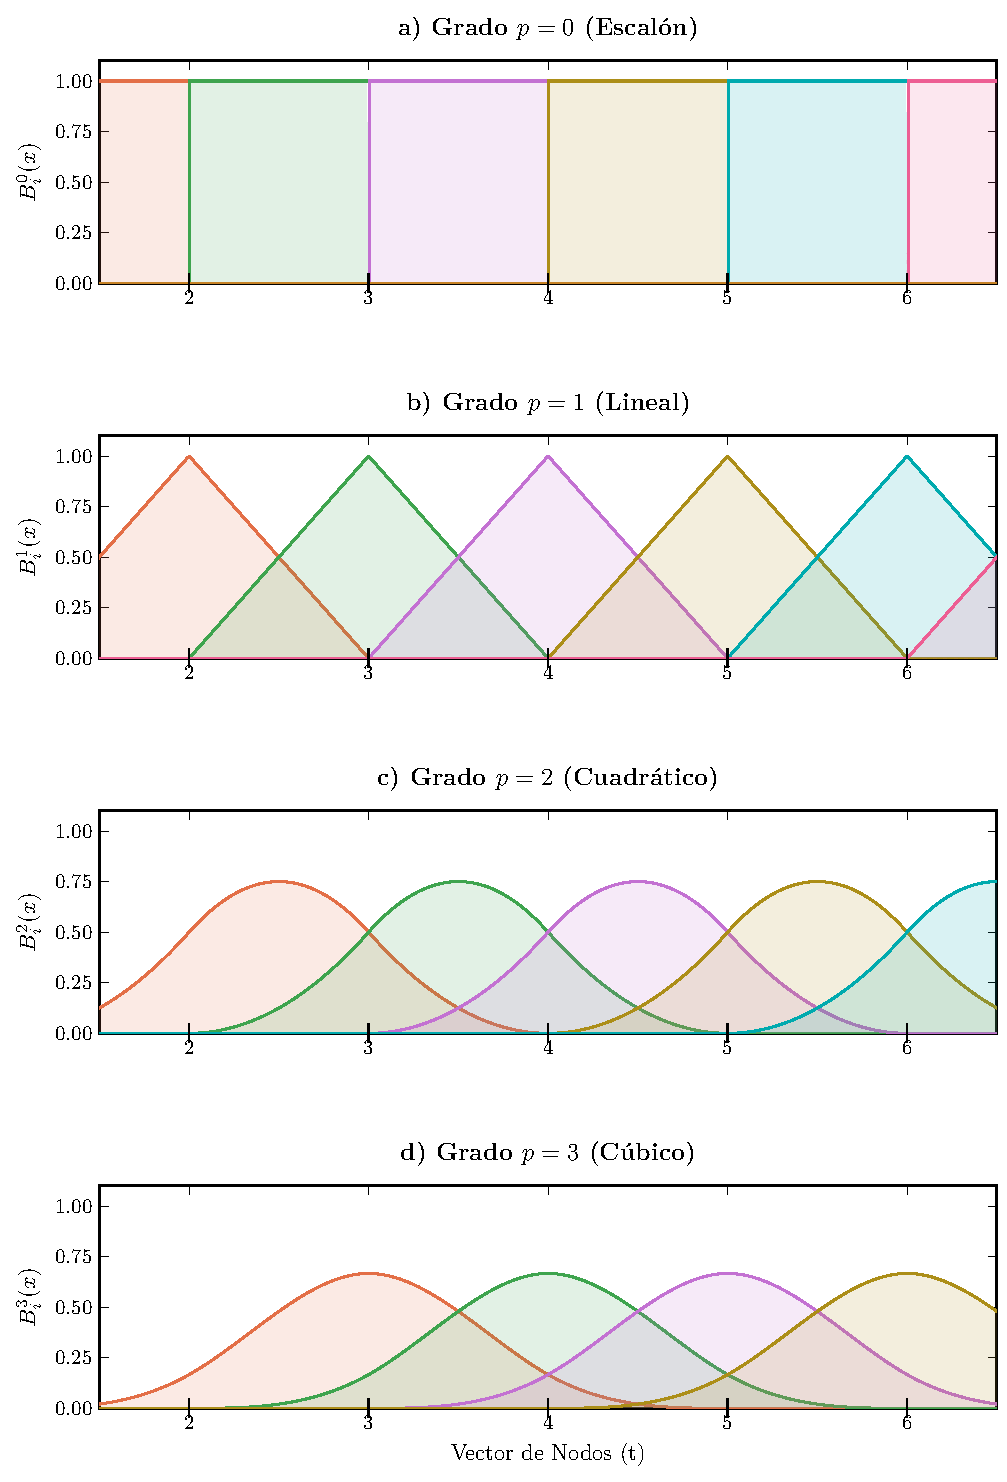
\includegraphics[width=0.8\textwidth]{figura_evolucion_splines.pdf}
    \caption{Evolución de las funciones base B-spline generadas mediante la fórmula de recurrencia de Cox-de Boor. \textbf{a)} Paso base ($p=0$) mostrando funciones escalón ortogonales. \textbf{b-d)} Aumento progresivo del grado ($p=1, 2, 3$) y de la regularidad $C^{p-1}$.}
    \label{fig:bspline-evolucion}
\end{figure}

\subsection{Soporte Compacto y Control Local}

La propiedad que distingue a los B-splines es su \textbf{soporte compacto}. A diferencia de las bases globales (STOs, GTOs), un B-spline $B_i^p(r)$ es estrictamente cero fuera del intervalo local $[t_i, t_{i+p+1})$. Esto significa que la función base solo vive sobre $p+1$ intervalos consecutivos de la malla.

Esta localidad tiene dos consecuencias:
\begin{enumerate}
    \item \textbf{Matrices Banda:} Al integrar el producto de dos funciones base, $\int B_i(r) B_j(r) dr$, el resultado es distinto de cero solo si sus soportes se intersectan ($|i-j| \leq p$). Las matrices resultantes (solapamiento, energía cinética) son matrices de banda (\textit{banded matrices}), con un ancho fijado por el orden del spline. Un solucionador que aproveche esa estructura resuelve un sistema lineal con costo $O(N)$ en lugar de $O(N^3)$; nuestro motor no la explota y almacena las matrices en formato denso, por las razones que se discuten en la Sección \ref{sec:repositorio}.
    \item \textbf{Control Local:} La alteración de un coeficiente $c_k$ en la expansión de la función de onda altera la curva \textit{exclusivamente} dentro de su región de influencia local $[t_k, t_{k+p+1})$. Esto permite resolver detalles finos, como el comportamiento cerca del núcleo, refinando la malla solo donde hace falta y sin introducir oscilaciones en el resto del dominio, a diferencia de lo que ocurre al elevar el grado de un interpolante polinómico global (fenómeno de Runge; ver Figura \ref{fig:control_local_fem}).
\end{enumerate}

Ambas propiedades son las que motivan el uso de esta base en física atómica, y la revisión de \textcite{Bachau2001} documenta con detalle su aplicación a problemas de estructura y de continuo. El fenómeno de Runge que el control local evita, consistente en la aparición de oscilaciones de amplitud creciente cerca de los extremos del dominio al elevar el grado de un interpolante polinómico global, es un resultado clásico del análisis numérico cuyo tratamiento en el contexto de splines puede consultarse en \textcite{deBoor1978}.

\begin{figure}[htbp]
    \centering
    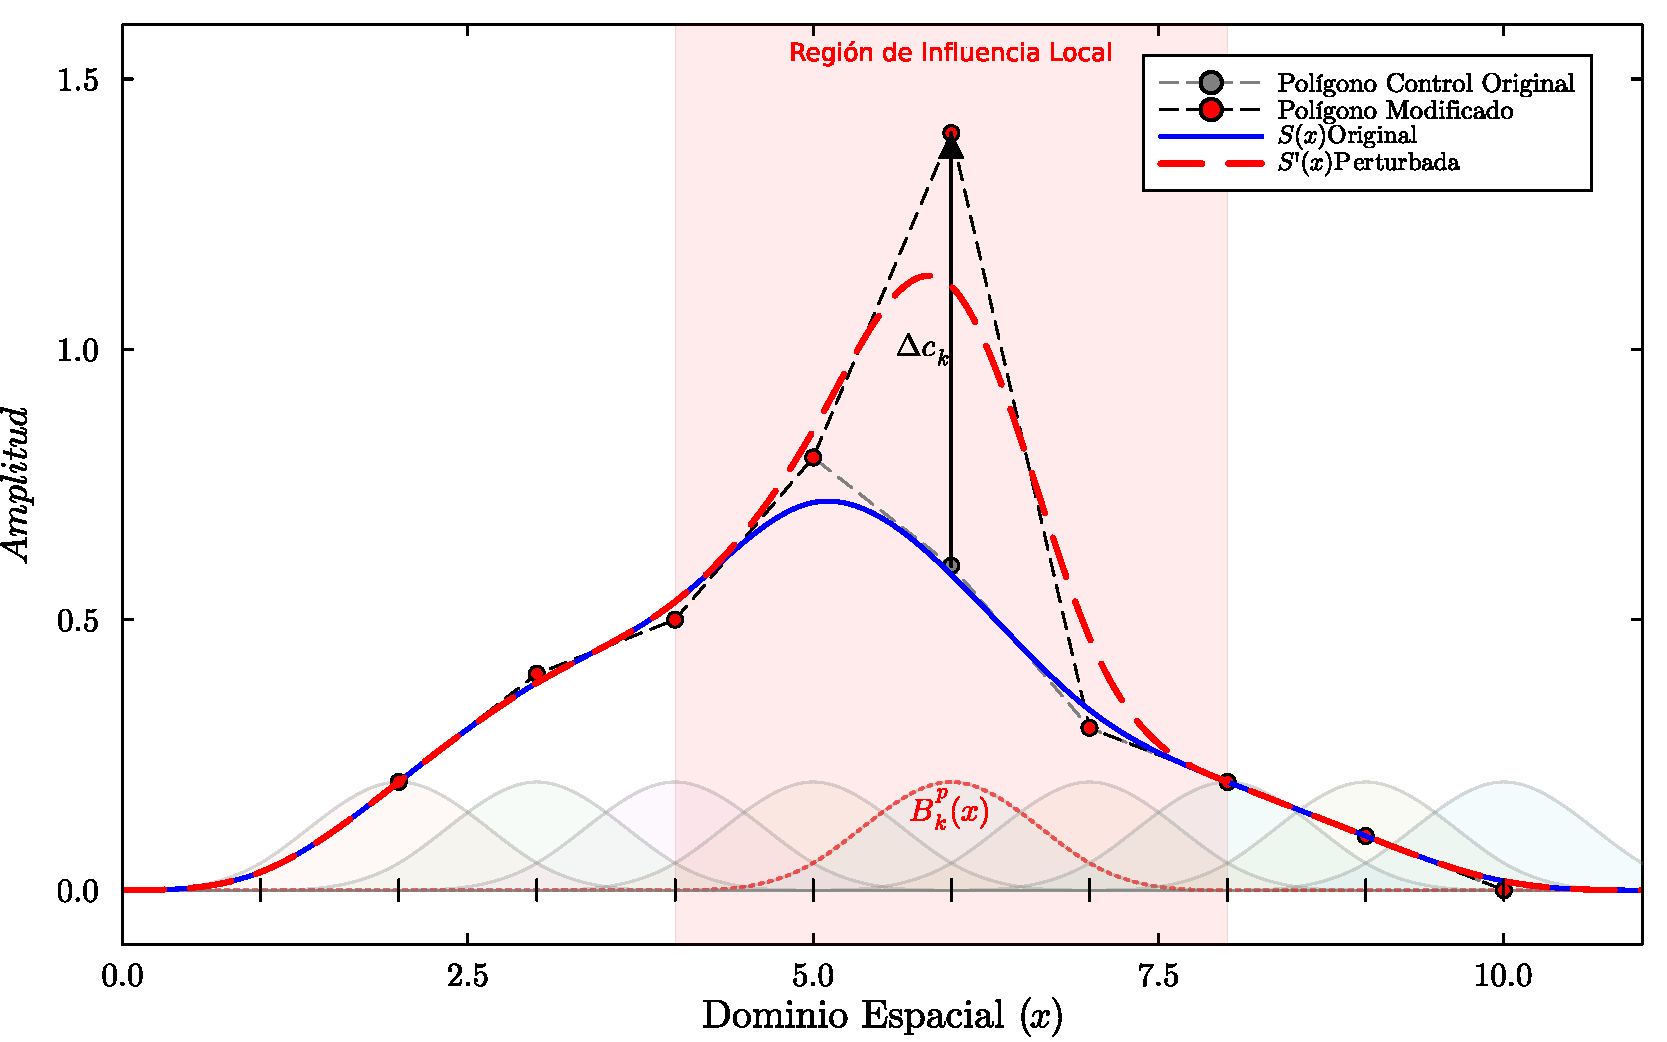
\includegraphics[width=0.9\textwidth]{figura_control_local_fem.pdf}
    \caption{Ilustración de la propiedad de control local en B-splines. La perturbación de un coeficiente $\Delta c_k$ altera la curva solución exclusivamente dentro de la \textbf{Región de Influencia Local} (área sombreada correspondiente al soporte compacto de $B_k^p$). Fuera de este intervalo, la curva no se ve afectada.}
    \label{fig:control_local_fem}
\end{figure}

\subsection{Malla Exponencial y Distribución de Nudos}

Para resolver eficientemente la ecuación radial atómica, es necesario adaptar la densidad de la base a la física del problema: se requiere alta resolución cerca del origen, donde el potencial coulombiano $-Z/r$ es singular y los orbitales internos varían en una escala $1/Z$, y menor resolución en la región asintótica. Siguiendo a \textcite{Bachau2001}, esto se logra mapeando una variable uniforme $\xi \in [0,1]$ al dominio físico radial mediante una transformación exponencial:
\begin{equation}
\label{eq:exp-grid}
    r(\xi) = R_{\text{max}} \frac{e^{\gamma \xi}-1}{e^{\gamma}-1},
\end{equation}
donde $\gamma$ controla cuánto se concentran los nudos cerca del origen. El jacobiano de esta transformación, $\dv*{r}{\xi} \propto e^{\gamma \xi}$, indica que el tamaño de cada intervalo crece exponencialmente al alejarse del núcleo (Figura \ref{fig:grid_comparison}). Los valores de $\gamma$, del número de intervalos y del orden del spline empleados en cada elemento se recogen en la Tabla \ref{tab:parametros_base}.

\begin{figure}[htbp]
    \centering
    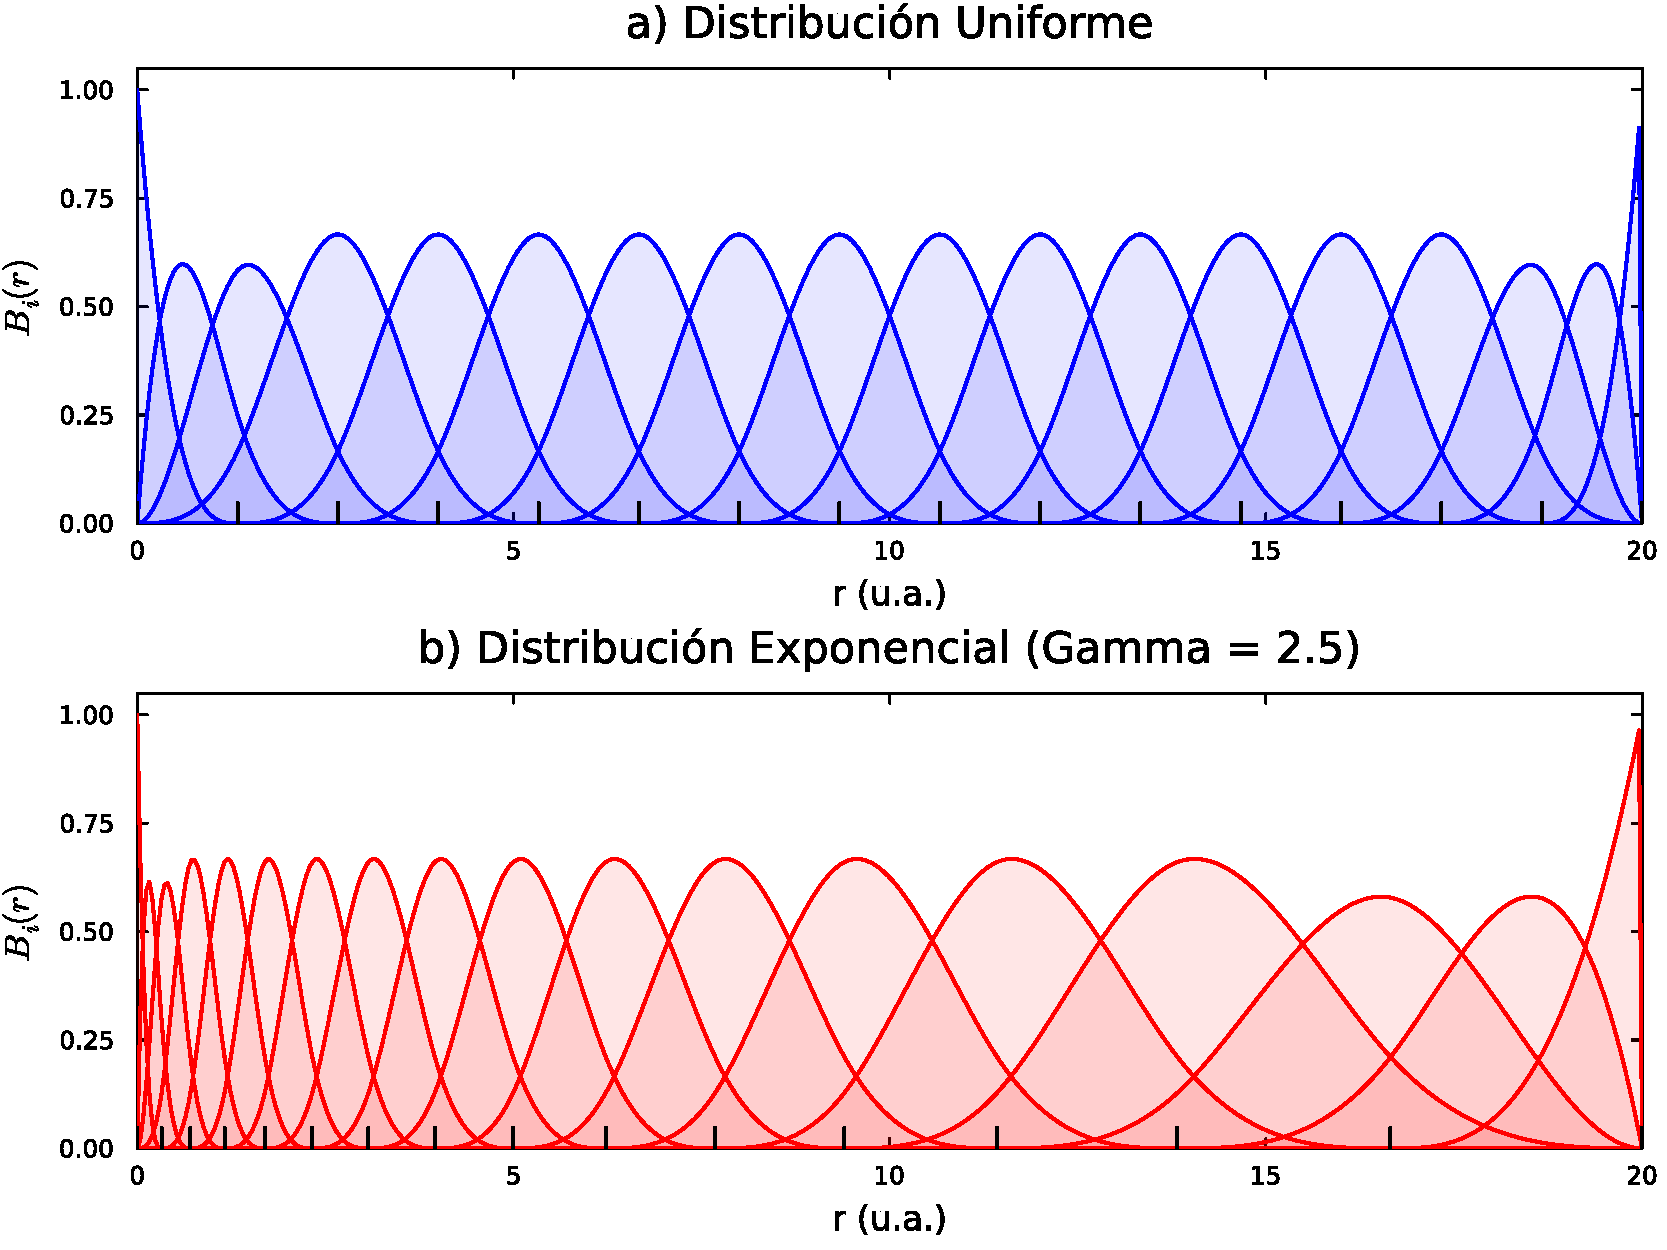
\includegraphics[width=0.85\textwidth]{figura_comparacion_mallas.pdf}
    \caption{\textbf{Comparación de distribuciones de nudos B-spline.} a) Distribución uniforme, ineficiente para orbitales atómicos. b) Distribución exponencial ($\gamma=2.5$), mostrando la alta densidad de bases requerida cerca del origen.}
    \label{fig:grid_comparison}
\end{figure}

\section{El Método de Galerkin}
\label{sec:galerkin}

Elegida la base, resta el problema de cómo proyectar sobre ella una ecuación diferencial. En este trabajo empleamos el \textbf{método de Galerkin}, una formulación del Método de Elementos Finitos (FEM) que discretiza de manera unificada tanto la ecuación de eigenvalores de Hartree-Fock como la ecuación de Poisson que determina los potenciales de interacción. Presentamos aquí el esquema y sus resultados; la demostración de su equivalencia con el principio variacional de Ritz y la deducción de la ecuación de Poisson radial se desarrollan en el Apéndice \ref{ap:galerkin-poisson}.

\subsection{Del problema continuo al problema matricial}

Partimos de la ecuación de Schrödinger radial \eqref{eq:radial_schrodinger}, deducida en la Sección \ref{sec:campo_central} a partir de la aproximación de campo central,

\begin{equation}
\label{eq:strong-form}
  \qty[ - \frac{1}{2}\dv[2]{r} + V_{\text{eff}}(r) ] P(r) = \epsilon P(r),
\end{equation}

donde $V_{\text{eff}}(r)$ contiene la atracción nuclear, el término centrífugo $l(l+1)/2r^2$ y el potencial de campo medio. Al sustituir la expansión finita en la base de B-splines,

\begin{equation}
\label{eq:expansion-metodo}
  P(r) \approx \tilde{P}(r) = \sum_{j=1}^{N} c_j B_j(r),
\end{equation}

la igualdad (\ref{eq:strong-form}) deja de satisfacerse de manera exacta: el subespacio finito generado por $\{B_j\}$ no contiene, en general, a la solución verdadera. La discrepancia define el \textbf{residuo}

\begin{equation}
\label{eq:residuo}
  R(r) = \qty[ - \frac{1}{2}\dv[2]{r} + V_{\text{eff}}(r) - \epsilon ] \tilde{P}(r) \neq 0.
\end{equation}

El método de Galerkin impone que este residuo sea ortogonal al subespacio de aproximación, tomando como funciones de peso las mismas funciones base:

\begin{equation}
\label{eq:galerkin-condition}
  \int_{0}^{R_{\text{max}}} B_i(r) R(r) \dd{r} = 0, \qquad i = 1, \dots, N.
\end{equation}

La interpretación geométrica es directa: al anular la proyección del error sobre cada función base, garantizamos que no quede ninguna componente del residuo que pudiéramos haber corregido ajustando los coeficientes $c_j$. El error remanente es entonces intrínseco al tamaño de la base, y no un defecto de la proyección.

El término cinético de (\ref{eq:galerkin-condition}) contiene una segunda derivada que tratamos mediante integración por partes,

\begin{equation}
\label{eq:ibp-metodo}
  \int_{0}^{R_{\text{max}}} B_i(r) \dv[2]{\tilde{P}}{r} \dd{r} = \underbrace{\eval{ B_i(r) \dv{\tilde{P}}{r} }_{0}^{R_{\text{max}}}}_{=\,0} - \int_{0}^{R_{\text{max}}} \dv{B_i}{r} \dv{\tilde{P}}{r} \dd{r},
\end{equation}

donde el término de borde se anula porque las funciones de prueba $B_i$ que se retienen se anulan en ambos extremos, la misma condición $P(0) = P(R_{\text{max}}) = 0$ que cumple la solución. Este paso, característico de la \textit{forma débil}, cumple dos funciones: rebaja el requisito de continuidad sobre la base (basta con que sea derivable una vez) y simetriza el operador, lo cual garantiza que la matriz resultante sea Hermitiana.

Sustituyendo la expansión (\ref{eq:expansion-metodo}) y factorizando los coeficientes, cada integral se convierte en un elemento de matriz:

\begin{align}
  \label{eq:matrix-elements}
  T_{ij} = \frac{1}{2}\int_{0}^{R_{\text{max}}} \dv{B_i}{r} \dv{B_j}{r} \dd{r} \qc & 
  V_{ij}= \int_{0}^{R_{\text{max}}} B_i(r)\, V_{\text{eff}}(r)\, B_j(r) \dd{r}, \\
  S_{ij} = \int_{0}^{R_{\text{max}}} & B_i(r) B_j(r) \dd{r}.
\end{align}

La condición de Galerkin para todo $i$ produce entonces el sistema $\sum_j (T_{ij} + V_{ij}) c_j = \epsilon \sum_j S_{ij} c_j$. Definiendo la matriz Hamiltoniana $H_{ij} = T_{ij} + V_{ij}$, el problema continuo se convierte en un \textbf{problema de eigenvalores generalizado}:

\begin{equation}
\label{eq:eigen-metodo}
  \bm{H}\bm{c} = \epsilon\, \bm{S}\bm{c}.
\end{equation}

La aparición de la matriz de solapamiento $\bm{S}$ en el lado derecho es consecuencia directa de que la base de B-splines no es ortogonal: a diferencia de una base ortonormal, $S_{ij} \neq \delta_{ij}$, y $\bm{S}$ define la métrica del espacio de Hilbert discretizado. Por el soporte compacto de la base, tanto $\bm{H}$ como $\bm{S}$ son matrices de banda con ancho determinado únicamente por el orden $k$ del spline.

\subsection{Aplicación: la ecuación de Poisson radial}
\label{subsec:poisson-metodo}

La misma maquinaria resuelve el segundo obstáculo del método de Hartree-Fock: la evaluación de las integrales de Slater que describen la repulsión electrón-electrón. Al expandir el operador de Coulomb $\abs{\bm{r}_i - \bm{r}_j}^{-1}$ en armónicos esféricos, la parte angular se resuelve analíticamente mediante el álgebra de momento angular, y toda la física radial queda contenida en el potencial multipolar de orden $k$ generado por la densidad de par $\rho_{ab}(r) = P_a(r)P_b(r)$:

\begin{equation}
\label{eq:Yk-metodo}
  Y^k(a,b;r) = r \int_0^\infty \frac{r_{<}^k}{r_{>}^{k+1}} P_a(s) P_b(s) \dd{s}.
\end{equation}

Evaluar (\ref{eq:Yk-metodo}) directamente por cuadratura es costoso y genera matrices densas, pues se trata de un operador integral \textit{global}: el valor del potencial en un punto depende de la densidad en todo el dominio. La alternativa que adoptamos explota el hecho de que $Y^k(a,b;r)$ es solución de una ecuación diferencial \textit{local}, la \textbf{ecuación de Poisson radial generalizada} (\ref{eq:poisson-true}):

\begin{equation}
\label{eq:poisson-metodo}
  \qty( -\dv[2]{r} + \frac{k(k+1)}{r^2} ) Y^k(a,b;r) = \frac{2k+1}{r} P_a(r) P_b(r),
\end{equation}

sujeta a la condición $Y^k(0) = 0$ en el origen y al comportamiento asintótico $Y^k \to M_k\,r^{-k}$, donde $M_k = \int_0^\infty s^k P_a(s)P_b(s) \dd{s}$ es el momento multipolar de la densidad de par. Como $M_k$ depende de la densidad que se está calculando, en el borde $R_{\text{max}}$ no se impone su valor sino una condición de Robin que lo elimina, la Ecuación \eqref{eq:robin} del Capítulo \ref{ch:ciclo-scf}. La equivalencia entre la definición integral (\ref{eq:Yk-metodo}) y la forma diferencial (\ref{eq:poisson-metodo}), junto con el comportamiento de $Y^k$ en los dos extremos del dominio, se demuestra en el Apéndice \ref{ap:galerkin-poisson}.

Proyectamos (\ref{eq:poisson-metodo}) sobre la base con el mismo procedimiento de la sección anterior. Multiplicando por $B_i(r)$, integrando por partes el término de segunda derivada y expandiendo $Y^k(r) \approx \sum_j y_j B_j(r)$, obtenemos la forma débil, salvo el término de borde en $R_{\text{max}}$, que aporta la condición de Robin,

\begin{equation}
\label{eq:poisson-weak-metodo}
  \sum_j \qty[ \int_0^{R_{\text{max}}} \dv{B_i}{r}\dv{B_j}{r} \dd{r} + k(k+1)\int_0^{R_{\text{max}}} \frac{B_i B_j}{r^2} \dd{r} ] y_j = (2k+1)\int_0^{R_{\text{max}}} \frac{B_i P_a P_b}{r} \dd{r},
\end{equation}

que en notación matricial es simplemente un sistema lineal,

\begin{equation}
\label{eq:poisson-linear-metodo}
  \bm{A}^{(k)} \bm{y} = \bm{b}, \qquad \bm{A}^{(k)} = 2\bm{T} + k(k+1)\bm{V}^{(2)},
\end{equation}

donde $\bm{T}$ es la misma matriz cinética de (\ref{eq:matrix-elements}) y $\bm{V}^{(2)}$ es la matriz del operador $r^{-2}$. El resultado tiene dos propiedades útiles. Primero, el operador $\bm{A}^{(k)}$ depende únicamente de la malla de nudos y del orden multipolar $k$: es completamente independiente de la densidad electrónica y, por lo tanto, invariante a lo largo del ciclo autoconsistente. Segundo, $\bm{A}^{(k)}$ hereda de la base la misma estructura de banda simétrica que $\bm{H}$ y $\bm{S}$ y es definida positiva, de modo que admite una factorización de Cholesky que se calcula una sola vez y se reutiliza durante todo el ciclo.

Así, un único formalismo variacional discretiza el operador de Fock y los potenciales de interacción $Y^k$, unificando la arquitectura del solucionador. En el Capítulo \ref{ch:ciclo-scf} explotamos la invariancia de $\bm{A}^{(k)}$ y de los operadores de un cuerpo para reorganizar el ciclo SCF como una secuencia de contracciones algebraicas.

%%% Local Variables:
%%% mode: LaTeX
%%% TeX-master: "../main"
%%% End:


% Capítulo 5: Implementación del Ciclo SCF y Correcciones
\chapter{Implementación del Ciclo SCF y Correcciones}
\label{ch:ciclo-scf}

\section{El Ciclo del Campo Autoconsistente (SCF)}

Como se vio en la Sección \ref{sec:fock_operator}, el operador de Fock depende de sus propias soluciones: no es posible obtener los orbitales sin conocer el potencial que ellos mismos generan, ni construir ese potencial sin los orbitales. El algoritmo de campo autoconsistente (SCF, \textit{Self-Consistent Field}) resuelve esa dependencia por iteración. Al proyectar las funciones radiales $P_a(r)$ sobre una base finita de dimensión $N$, las ecuaciones integro-diferenciales de campo medio se transforman en las ecuaciones matriciales de \textcite{Roothaan1960}:

\begin{equation}
  \bm{F}\bm{c} = \epsilon\bm{S}\bm{c},
\end{equation}

donde $\bm{c}$ es el vector columna que contiene los coeficientes de expansión del orbital, $\bm{S}$ es la matriz de traslape (\textit{overlap}) de las funciones base, y $\bm{F}$ es la Matriz de Fock. La matriz de Fock es el análogo discreto del Hamiltoniano efectivo, y su construcción depende de la matriz de densidad $\bm{D}$, la cual se forma a partir de los vectores $\bm{c}$ de los estados ocupados.

La transición desde la ecuación diferencial analítica de Hartree-Fock hacia la formulación matricial de Roothaan-Hall se obtiene aplicando el método de Galerkin desarrollado en el Capítulo \ref{ch:bsplines-galerkin}. Al proyectar el operador de Fock sobre las funciones de prueba de la base, los elementos matriciales son

\begin{equation}
\label{eq:fock-matrix-elements}
  F_{ij} = \int_0^{R_{\text{max}}} B_i(r)\, \hat{f}\, B_j(r) \dd{r},
\end{equation}

y la matriz de solapamiento $\bm{S}$ es la ya definida en la Ec. (\ref{eq:matrix-elements}). La diferencia esencial respecto al problema de un cuerpo de la Ec. (\ref{eq:eigen-metodo}) es que $\hat{f}$ depende de los orbitales que precisamente buscamos: lo que en el Capítulo \ref{ch:bsplines-galerkin} era un problema lineal de eigenvalores se convierte aquí en uno no lineal, que solo puede resolverse por iteración.

El algoritmo procede de la siguiente manera:

\begin{enumerate}
    \item \textbf{Punto de partida:} El ciclo necesita un conjunto inicial de orbitales. Lo obtenemos diagonalizando, sobre la misma base de B-splines, el Hamiltoniano de un cuerpo del núcleo desnudo, sin repulsión entre electrones; son orbitales hidrogenoides de carga $Z$, que tienen ya la estructura de nodos correcta, y con ellos se forma la densidad inicial.
    \item \textbf{Construcción del operador de Fock:} Con los orbitales de la iteración en curso se resuelven las ecuaciones de Poisson, se construyen las matrices de Coulomb y de intercambio y, al sumar el Hamiltoniano de un cuerpo, se ensambla la matriz $\bm{F}$ de cada bloque.
    \item \textbf{Diagonalización:} Se resuelve el problema generalizado de eigenvalores $\bm{F}\bm{c} = \epsilon\bm{S}\bm{c}$, que entrega un nuevo conjunto de coeficientes $\bm{c}$ y de energías orbitales $\epsilon$.
    \item \textbf{Criterio de autoconsistencia:} Con los orbitales nuevos se calcula la energía total. Si difiere de la de la iteración anterior en más que una tolerancia, se regresa al paso 2 con los orbitales nuevos; el ciclo termina cuando ese cambio cae por debajo de la tolerancia.
\end{enumerate}

\begin{figure}[p]
  \centering
  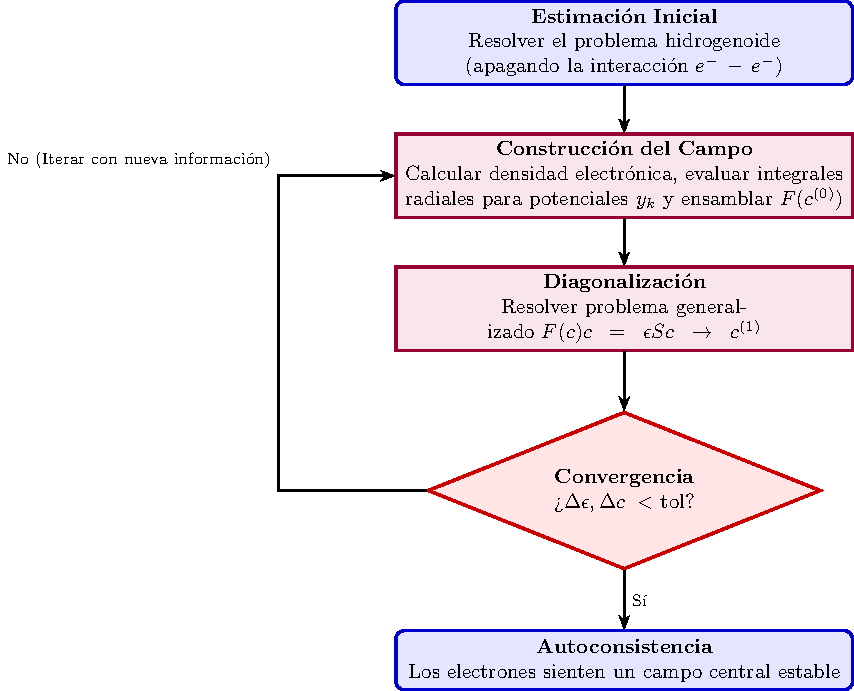
\includegraphics[width=1.0\textwidth]{scf}
  \caption{Diagrama de flujo del ciclo de campo autoconsistente (SCF). El proceso comienza con los orbitales del problema hidrogenoide, sin repulsión entre electrones, y avanza cíclicamente por la formación de los operadores de Coulomb e intercambio y la diagonalización de la matriz de Fock. El ciclo concluye cuando el cambio entre iteraciones cae por debajo de la tolerancia; en la implementación el criterio se aplica a la energía total.}
  \label{fig:scf-cycle}
\end{figure}

\subsection{Amortiguación de Oscilaciones: Level-Shifting}
\label{sec:level_shifting}

El carbono y el silicio convergen en unas decenas de iteraciones sin ninguna ayuda. En el germanio y el estaño el ciclo se estabiliza con el desplazamiento de nivel (\textit{level shifting}) de \textcite{Saunders1973}, que eleva las energías del espacio virtual y deja intacto el espacio ocupado. La técnica previene un modo de fallo conocido del ciclo simple: cuando una variación de la matriz de densidad $\bm{D}$ altera el orden de los autovalores de un bloque, el principio de construcción ocupa un autovector distinto en iteraciones sucesivas y el ciclo alterna entre dos densidades sin converger a ninguna.

Si denotamos como $\bm{R}_v$ al proyector sobre el subespacio virtual, definimos la matriz de Fock desplazada como:

\begin{equation}
    \bm{F}^{\text{shift}} = \bm{F} + \lambda \bm{S} \bm{R}_v \bm{S},
\end{equation}

donde $\lambda > 0$ es el parámetro de desplazamiento, y $\bm{S}$ es la matriz de solapamiento de la base no ortogonal de B-splines.

En la base de los orbitales de la iteración anterior, la transformación equivale a sumar la constante $\lambda$ a las energías de los orbitales desocupados, $\epsilon_a \rightarrow \epsilon_a + \lambda$. En nuestras corridas el germanio y el estaño emplean $\lambda = 3.0$ Hartree, mientras que el carbono y el silicio convergen sin desplazamiento. Un desplazamiento suficientemente grande ensancha la separación entre ocupados y virtuales, impide los cruces de niveles y amortigua las oscilaciones. Como el término $\lambda\bm{S}\bm{R}_v\bm{S}$ no actúa sobre el espacio ocupado, el punto fijo es el mismo con y sin desplazamiento y las energías convergidas son las del Hartree-Fock restringido de capa abierta; lo que cambia es la trayectoria, y con ella el número de iteraciones.

\subsection{Extrapolación de Pulay sobre el Conmutador Proyectado}
\label{sec:cdiis_metodo}

El desplazamiento de nivel estabiliza el ciclo pero no lo acelera: al ampliar la brecha artificialmente también reduce el paso efectivo de cada iteración, y mantenido durante todo el ciclo lleva la convergencia del germanio y del estaño a cerca de doscientas cincuenta iteraciones (Tabla \ref{tab:cdiis}). La técnica que resuelve el problema de fondo es la extrapolación de Pulay \parencite{Pulay1980}, que en lugar de amortiguar la iteración construye, a partir del historial de matrices de Fock, la combinación lineal que más se acerca al punto fijo. En su segunda formulación \parencite{Pulay1982} la medida del error es el conmutador entre la matriz de Fock y la de densidad, y por eso se la conoce como C-DIIS.

En un Hartree-Fock de capa cerrada el vector de error es $\bm{e} = \bm{F}\bm{D}\bm{S} - \bm{S}\bm{D}\bm{F}$, que se anula exactamente en la solución porque allí los orbitales ocupados generan un subespacio invariante del único operador de Fock. Nuestro esquema ROHF no cumple esa condición. Como se describe en la Sección \ref{sec:gram-schmidt}, el orbital de valencia se obtiene como autovector $\bm{v}$ de su propio operador, $\bm{F}_{np}\bm{v} = \epsilon\,\bm{S}\bm{v}$, y después se ortogonaliza contra los orbitales del core del mismo momento angular, que provienen de un operador distinto. El orbital que resulta, proporcional a $\bm{v} - \sum_c (\bm{c}_c^{T}\bm{S}\bm{v})\,\bm{c}_c$, ya no es autovector de $\bm{F}_{np}$, y en el punto fijo satisface

\begin{equation}
    \label{eq:rohf_lagrange}
    \bm{F}_{np}\,\bm{c}_{np} = \epsilon\,\bm{S}\,\bm{c}_{np} + \sum_{c \in \text{core}} a_c \left( \epsilon\,\bm{S} - \bm{F}_{np} \right) \bm{c}_{c},
\end{equation}

donde cada coeficiente $a_c$ es proporcional al solapamiento $\bm{c}_c^{T}\bm{S}\bm{v}$ que la ortogonalización elimina. El segundo término impide que el conmutador crudo baje de un piso no nulo, que en las trazas registradas es de $4.4\times10^{-5}$ para el silicio, $2.2\times10^{-6}$ para el germanio y $7.1\times10^{-7}$ para el estaño. Una extrapolación construida sobre vectores de error que han dejado de decrecer no converge, porque ya no distingue las iteraciones mejores de las peores.

El carbono funciona como control de este diagnóstico. Es el único elemento de la secuencia cuyo core carece de electrones $p$, de modo que su orbital de valencia no requiere ortogonalización contra el core y la suma de la Ecuación \eqref{eq:rohf_lagrange} está vacía; su conmutador crudo no tiene piso y sigue bajando con la convergencia, hasta $1.1\times10^{-13}$ al detenerse el ciclo, más de ocho órdenes de magnitud por debajo del piso del silicio. El piso no es entonces un artefacto de la base ni de la malla, sino la huella del esquema de ortogonalización, la misma que reaparece en los momentos radiales del Capítulo \ref{ch:resultados}.

El remedio consiste en proyectar el error fuera del espacio ocupado antes de usarlo. Si $\bm{C}_{\text{occ}}$ reúne en columnas todos los orbitales ocupados del mismo momento angular, tanto los del core como el de valencia, el vector de error proyectado es

\begin{equation}
    \label{eq:cdiis_error}
    \bm{e} = \left( \bm{1} - \bm{S}\,\bm{C}_{\text{occ}}\bm{C}_{\text{occ}}^{T} \right)\left( \bm{F}\bm{D}\bm{S} - \bm{S}\bm{D}\bm{F} \right) = \left( \bm{1} - \bm{S}\,\bm{C}_{\text{occ}}\bm{C}_{\text{occ}}^{T} \right)\bm{F}\bm{D}\bm{S},
\end{equation}

donde el segundo sumando se anula de manera idéntica porque $\bm{S}\bm{D}\bm{F}$ vive por completo en el espacio ocupado. Lo que queda es el bloque ocupado-virtual del gradiente orbital. La proyección elimina la parte del segundo término de la Ecuación \eqref{eq:rohf_lagrange} que vive en el espacio ocupado, que es la dominante, pero no su componente virtual, de modo que el error proyectado tampoco se anula exactamente: se estanca en $7.8\times10^{-8}$ en el silicio, $1.6\times10^{-9}$ en el germanio y $5.3\times10^{-10}$ en el estaño, unos tres órdenes de magnitud por debajo del conmutador crudo. Ese margen es el que permite a la extrapolación actuar antes de tocar el piso.

La segunda particularidad de nuestro esquema es que la extrapolación opera por bloques. Cada canal tiene su propio operador de Fock y su propia matriz de densidad, y la capa abierta $np$ convive con un canal de core del mismo momento angular sobre el mismo espacio activo; construir un solo vector de error mezclando ambos invalidaría el conmutador. Cada canal aporta entonces su matriz de error a partir de su pareja $(\bm{F}, \bm{D})$, y el sistema de Pulay se resuelve sobre el historial conjunto, conservando las matrices de Fock sin desplazar. El historial se limita a seis iteraciones y se descarta cuando el condicionamiento del sistema o la magnitud de los coeficientes indican que los vectores de error se han vuelto casi paralelos.

El cambio entre los dos regímenes se decide por el residual y no por un número fijo de iteraciones. Mientras el error proyectado permanece por encima de $10^{-2}$, el desplazamiento de nivel de la Sección \ref{sec:level_shifting} mantiene al sistema dentro de la cuenca de atracción; en cuanto baja de ese umbral el shift se apaga y la extrapolación toma el control. Cuando el error proyectado deja de mejorar durante seis iteraciones consecutivas, señal de que ha tocado su piso, la extrapolación se desactiva y el tramo final lo recorre el ciclo simple. El método tiene además un límite que hay que señalar: se trata de C-DIIS por bloques sobre operadores de Fock dependientes del término, y no del método canónico, ya que no existe un operador único que diagonalizar y el acoplamiento entre la capa abierta y las cerradas no entra en el residual. Por esa razón la convergencia se declara siempre sobre la energía total, y el residual se emplea únicamente para decidir el cambio de régimen. El efecto medido sobre el conteo de iteraciones, y la comprobación de que ambos regímenes llegan a la misma energía, se documentan en la Sección \ref{sec:cdiis_resultados}.

\section{Estructura Algebraica del Ciclo Autoconsistente}
\label{sec:estructura-algebraica}

Todas las integrales que aparecen en esta sección se evalúan por cuadratura de Gauss-Legendre sobre cada intervalo de la malla, con $N_q = k+6$ puntos por intervalo. Una regla de $N_q$ puntos integra exactamente polinomios de grado hasta $2N_q - 1 = 2k+11$, de modo que las matrices de solapamiento y cinética, cuyos integrandos son polinomios a trozos de grado a lo sumo $2k-2$, se obtienen sin error de cuadratura. Los integrandos con factores $1/r$, $1/r^2$ o $r^{-4}$, y los productos triples del tensor de interacción del Apéndice \ref{ap:bsplines}, no son polinómicos; para ellos los puntos adicionales reducen el error de cuadratura sin anularlo, y el acuerdo de las energías y de las integrales de Slater con la referencia (Tablas \ref{tab:resultados_energia_global} y \ref{tab:parametros_radiales}) acota su efecto. El detalle del mapeo afín al intervalo de referencia se encuentra en la Sección \ref{sec:gauss-legendre} del Apéndice \ref{ap:metodos-auxiliares}.

Cada iteración del ciclo reconstruye la matriz de Fock y resuelve las ecuaciones de Poisson que definen los potenciales de interacción, pero las funciones base y la cuadratura con que se integran permanecen fijas. Eso permite separar de manera exacta lo que depende de la geometría de la base de lo que depende del estado del átomo: las matrices de un cuerpo se calculan una sola vez, y el término fuente de la ecuación de Poisson se obtiene contrayendo un tensor geométrico precalculado con la matriz de densidad, sin reconstruir la densidad sobre la malla (Sección \ref{sec:tensores_geometria} del Apéndice \ref{ap:bsplines}). Lo que sigue describe la parte de ese esquema que tiene contenido físico, el operador de Poisson y sus condiciones de frontera.

\subsection{El operador de Poisson y sus condiciones de frontera}

Construido el término fuente, resta invertir el operador diferencial. Como se estableció en la Ec. (\ref{eq:poisson-linear-metodo}), la representación matricial del operador de Poisson para el multipolo de orden $k$ es

\begin{equation}
  \bm{A}^{(k)} = 2\bm{T} + k(k+1)\bm{V}^{(2)},
\end{equation}

donde $\bm{V}^{(2)}$ es la matriz del operador $r^{-2}$. Esta matriz depende exclusivamente de la secuencia de nudos y del orden multipolar, y es por tanto invariante a lo largo del ciclo. Para las condiciones de frontera físicas del átomo, $\bm{A}^{(k)}$ es simétrica definida positiva, lo que admite su descomposición de Cholesky

\begin{equation}
  \bm{A}^{(k)} = \bm{L}_k \bm{L}_k^{T},
\end{equation}

que nuestra implementación calcula una sola vez para cada multipolo $k$ requerido y conserva en memoria durante todo el ciclo. En las iteraciones subsecuentes, obtener el potencial se reduce a dos sustituciones triangulares sobre la factorización ya conocida. Con el almacenamiento denso que emplea el motor (Sección \ref{sec:repositorio}) su costo es cuadrático en el número de splines, frente al costo cúbico de refactorizar en cada paso.

Resta imponer las condiciones de frontera, y la base de B-splines permite hacerlo sin añadir ecuaciones al sistema. En el origen, el comportamiento $Y^k(r) \sim r^{k+1}$ deducido en el Apéndice \ref{ap:galerkin-poisson} se impone de manera exacta restringiendo el sistema a los splines con índice mayor que $k+1$, ya que son precisamente los primeros $k+1$ los que tienen valor o derivadas no nulas en $r=0$. La condición no se aplica entonces como una ecuación adicional sino eliminando del espacio de prueba las funciones que la violarían, lo que además reduce el tamaño del sistema en lugar de aumentarlo.

En el extremo exterior la situación es distinta, porque el valor del potencial en $R_{\text{max}}$ no se conoce de antemano: depende del momento multipolar $M_k$ de la densidad, que es justamente parte de lo que se está calculando. Lo que sí se conoce es la forma de la cola, $Y^k \to M_k r^{-k}$, y derivarla elimina la constante desconocida:

\begin{equation}
\label{eq:robin}
  \left. \dv{Y^k}{r} \right|_{R_{\text{max}}} + \frac{k}{R_{\text{max}}}\, Y^k(R_{\text{max}}) = 0 .
\end{equation}

La Ecuación \eqref{eq:robin} es una condición de Robin, y su virtud práctica es que en la formulación débil el término de borde se traduce en sumar $k/R_{\text{max}}$ a un único elemento diagonal de $\bm{A}^{(k)}$, el último. La matriz permanece simétrica y definida positiva, de modo que la factorización de Cholesky sigue siendo válida y el potencial ajusta su propia normalización sin que haya que suministrarla. Para el monopolo la condición degenera en una de Neumann, $\dd Y^0/\dd r = 0$, que es la condición natural de la formulación débil y que reproduce correctamente el límite $Y^0 \to M_0$ constante. Con estos elementos, cada iteración del ciclo autoconsistente se reduce a formar los términos fuente, resolver los sistemas de Poisson mediante sustitución triangular sobre las factorizaciones precalculadas, ensamblar la matriz de Fock y diagonalizarla.

\section{Implementación de Correcciones y Post-HF}

Con los orbitales convergidos del ciclo autoconsistente se calculan las correcciones que determinan el espectro: la correlación de la pareja de valencia, el acoplamiento espín-órbita y la polarización del core. Las dos primeras se aplican después del ciclo, sobre orbitales fijos, mientras que la tercera modifica el Hamiltoniano de un cuerpo y exige repetir el ciclo. Esta sección describe la implementación de cada una.

\subsection{Implementación de Interacción de Configuraciones (CI) y Acoplamiento Espín-Órbita (SO)}
\label{sec:ci_method}

El procedimiento trata por separado la correlación de valencia y el acoplamiento espín-órbita, en dos etapas sucesivas, y en ambas el core permanece congelado. En la primera se corrige la parte electrostática con el modelo de la Sección \ref{sec:ci_teoria}. Se construye el operador de Fock de core congelado y se extraen de su diagonalización, para cada momento angular $l \le l_{\max}$, los orbitales virtuales; los primeros de cada canal forman, junto con el orbital de valencia, el espacio activo de $m$ orbitales por canal, y con él se generan todas las funciones de pareja de paridad par que pueden acoplarse al término considerado. La matriz del Hamiltoniano entre estas funciones se ensambla con la expresión de la Sección \ref{sec:ci_racah}, que reduce cada elemento a símbolos $6j$ e integrales radiales $R^k$ entre los orbitales del espacio activo. Esas integrales se calculan con el mismo resolvedor de Poisson del ciclo autoconsistente y se guardan en una caché, y su número es lo que fija el costo del cálculo (Sección \ref{sec:costo_ci}). La diagonalización arroja las energías correlacionadas $E_{\text{CI}}(^3P)$, $E_{\text{CI}}(^1D)$ y $E_{\text{CI}}(^1S)$, y su efecto neto es una compresión del espectro: en los cuatro elementos las separaciones entre términos quedan entre un $66\%$ y un $84\%$ de las de Hartree-Fock.

En la segunda etapa se introduce el acoplamiento espín-órbita. Las energías correlacionadas de la etapa anterior entran como elementos diagonales de las matrices de Breit-Pauli \eqref{eq:bp_j0}, \eqref{eq:bp_j2} y \eqref{eq:bp_j1} deducidas en la Sección \ref{sec:matrices_bp}, cuyos elementos fuera de la diagonal se construyen con el parámetro $\zeta_{np}$ evaluado sobre los orbitales convergidos según la Ecuación \eqref{eq:zeta_spin_orbit}. Cada bloque de $J$ se diagonaliza por separado. Este orden importa: aplicar el espín-órbita sobre energías ya correlacionadas, y no sobre las de Hartree-Fock puro, incrementa la mezcla singlete-triplete, porque la compresión electrostática de la primera etapa reduce el denominador que separa los estados acoplados.

De la diagonalización se extraen dos productos. Los eigenvalores conforman el espectro multiplete que se contrasta contra el NIST en el Capítulo \ref{ch:resultados}. Los eigenvectores proporcionan los coeficientes de mezcla entre los términos puros, con los que se calcula el factor de Landé efectivo que se analiza en la Sección \ref{sec:lande} y que mide el grado de mezcla en cada elemento de la secuencia.

\subsection{Implementación Empírica del Potencial de Polarización}
\label{sec:impl_polarizacion}

El campo medio con core congelado omite la correlación entre la valencia y las capas internas, que la Sección \ref{sec:core_polarization} describe como polarización del core. Tratarla desde primeros principios exigiría ampliar el cálculo de correlación con excitaciones del core o recurrir a la teoría de perturbaciones de muchos cuerpos, ambos fuera del alcance de este trabajo. En su lugar la representamos mediante el potencial semiempírico $V_{\text{pol}}(r)$ de la Ecuación \eqref{eq:vpol_cutoff}, que por ser local y depender solo de $r$ se suma a la atracción nuclear $-Z/r$ para formar un \textbf{potencial central efectivo}:

\begin{equation}
    \label{eq:vpol_efectivo}
    V_{\text{eff}}(r) = -\frac{Z}{r} - \frac{\alpha_d}{2 r^4} \left( 1 - e^{-(r/r_c)^6} \right).
\end{equation}

Este potencial sustituye a la atracción nuclear en la matriz del Hamiltoniano de un cuerpo $\hat{h}$:
\begin{equation}
    h_{ij} = \int_0^{R_{\text{max}}} B_i(r) \left[ -\frac{1}{2}\frac{d^2}{dr^2} + \frac{l(l+1)}{2r^2} + V_{\text{eff}}(r) \right] B_j(r) \dd{r}.
\end{equation}

En consecuencia, el ciclo SCF converge hacia una solución distinta, en la que los orbitales sienten la atracción adicional del core polarizado. Como el término entra en $\hat{h}$, actúa sobre todos los orbitales y no solo sobre los de valencia, que es donde lo sitúa el modelo de \textcite{Muller1984}: los orbitales del propio core también lo perciben. El corte $W_6$ lo suprime en las capas más internas, pero no en la subcapa $ns^2$ del core, cuya densidad se concentra fuera de $r_c$, y solo en parte en la $(n-1)d^{10}$ que la precede; esta aproximación de la implementación se suma a las limitaciones del parámetro $\alpha_d$ que se discuten en la Sección \ref{sec:limitaciones}.

Para operar este modelo hay que fijar los dos parámetros empíricos. El radio de corte $r_c$ representa el tamaño del core y evita la divergencia no física de $1/r^4$ cerca del núcleo. No lo ajustamos: lo mantenemos fijo en $r_c = 1.0\,a_0$ para el germanio y el estaño, de modo que la calibración recae sobre un solo grado de libertad.

La polarizabilidad $\alpha_d$ se extrae idealmente de mediciones sobre el ión de core cerrado análogo o de cálculos independientes de alta precisión. Para los cores de $\mathrm{Ge}$ y $\mathrm{Sn}$ no dispusimos de un valor de referencia verificable, de manera que la determinamos por ajuste espectroscópico: se repite el ciclo autoconsistente completo, y con él el cálculo CI posterior, para una rejilla de valores de $\alpha_d$, y se retiene el que minimiza el error cuadrático medio de los dos intervalos del término $^3P$ frente a los niveles del NIST. El barrido resultante y el valor adoptado en cada elemento se presentan en la Sección \ref{sec:vpol_resultados}. Un parámetro obtenido de este modo no es una polarizabilidad medida sino una cantidad efectiva, y que el Capítulo \ref{ch:resultados} documenta en qué sentido absorbe física ajena a la polarización del core.

\section{La Base de Datos de Espectros Atómicos del NIST (ASD)}
\label{sec:nist_asd}

Los niveles calculados se contrastan con los de la base \textit{Atomic Spectra Database} (ASD) del Instituto Nacional de Estándares y Tecnología de los Estados Unidos \parencite{NIST_ASD}. El ASD recopila y evalúa críticamente datos de espectroscopía de la literatura, y tabula para cada nivel medido su configuración, su término de Russell-Saunders dominante ($^{2S+1}L_J$) y su energía referida al estado fundamental. Los valores que el capítulo de resultados identifica como ``NIST'' proceden de la versión 5.12, consultada el 13 de septiembre de 2026, para los átomos neutros C I, Si I, Ge I y Sn I; de la misma consulta proceden las energías de ionización y los factores $g$. Los valores empleados, con la referencia primaria de cada nivel, quedaron registrados en el archivo de configuración que alimenta la generación de las tablas.

%%% Local Variables:
%%% mode: LaTeX
%%% TeX-master: "../main"
%%% End:


\part{Resultados y Análisis}
% Capítulo 6: Resultados y discusión
\chapter{Resultados y Discusión}
\label{ch:resultados}

Este capítulo presenta los resultados del motor numérico para la secuencia $np^2$, formada por el carbono ($Z=6$), el silicio ($Z=14$), el germanio ($Z=32$) y el estaño ($Z=50$), y los interpreta en términos de las aproximaciones del modelo. El orden sigue el del cálculo. Primero se establece que el campo medio reproduce el límite Hartree-Fock no relativista (Sección \ref{sec:validacion_hf}); después se construye el espectro de la configuración y se contrasta con el experimento (Sección \ref{sec:espectro}), se sigue el tránsito del acoplamiento $LS$ al intermedio a lo largo de la secuencia (Sección \ref{sec:regimen_acoplamiento}) y se examina el parámetro de espín-órbita junto con la corrección de polarización del core (Sección \ref{sec:zeta_diagnostico}). La Sección \ref{sec:limitaciones} reúne las limitaciones que explican las discrepancias restantes.

\section{El Límite de Hartree-Fock}
\label{sec:validacion_hf}

Antes de extraer cualquier parámetro espectroscópico hay que establecer que el estado fundamental que produce el motor es correcto. La validación descansa en dos criterios. El primero es la comparación de la energía total con los valores de \textcite{fischer1977}, referencia estándar del límite Hartree-Fock no relativista. El segundo es el cociente del virial $-V/T$, que por el teorema de la Sección \ref{sec:virial} vale exactamente $2$ para un sistema coulombiano y cuya desviación mide a la vez la convergencia del ciclo y la capacidad de la malla para representar la región nuclear y la cola asintótica de la función de onda.

\begin{table}[htbp]
    \centering
    % GENERADO por benchmarks/np2_sequence/tesis/etapa3_tablas.jl; no editar a mano.
% Procedencia:
%   carbon_rohf_results_3P_R30.0.jld2 (sha256 e8c5884b)
%   silicon_rohf_results_3P_R30.0.jld2 (sha256 09adeb32)
%   germanium_rohf_results_3P_R30.0.jld2 (sha256 7567c491)
%   tin_rohf_results_3P_R30.0.jld2 (sha256 7db46b8f)
%   Referencias: Froese Fischer (1977), copiadas en tesis/config.jl.
\begin{tabular}{l l S[table-format=-4.8] S[table-format=-4.10] S[table-format=1.1e-1]}
    \toprule
    \textbf{Elemento} & \textbf{Magnitud} & {\textbf{Este trabajo}} & {\textbf{Froese Fischer}} & {$|\Delta|$} \\
    \midrule
    \multirow{3}{*}{Carbono}
     & $E$ ($E_h$) & -37.68861896 & -37.688619 & 3.6e-8 \\
     & $T$ ($E_h$) & 37.68861897 & 37.688619 & 3.1e-8 \\
     & $-V/T$ & 2.00000000 & 1.999999998 & 1.9e-9 \\
    \midrule
    \multirow{3}{*}{Silicio}
     & $E$ ($E_h$) & -288.85435715 & -288.85436 & 2.8e-6 \\
     & $T$ ($E_h$) & 288.85878586 & 288.85437 & 4.4e-3 \\
     & $-V/T$ & 1.99998467 & 1.999999965 & 1.5e-5 \\
    \midrule
    \multirow{3}{*}{Germanio}
     & $E$ ($E_h$) & -2075.35973302 & -2075.3597 & 3.3e-5 \\
     & $T$ ($E_h$) & 2075.36257014 & 2075.3597 & 2.9e-3 \\
     & $-V/T$ & 1.99999863 & 2.00000005 & 1.4e-6 \\
    \midrule
    \multirow{3}{*}{Estaño}
     & $E$ ($E_h$) & -6022.93169410 & -6022.9317 & 5.9e-6 \\
     & $T$ ($E_h$) & 6022.93543641 & 6022.9316 & 3.8e-3 \\
     & $-V/T$ & 1.99999938 & 2.0000000019 & 6.2e-7 \\
    \bottomrule
\end{tabular}

    \caption{Energía total, energía cinética y cociente del virial frente a los valores de \textcite{fischer1977}. La última columna es la diferencia absoluta, en Hartree para $E$ y $T$.}
    \label{tab:resultados_energia_global}
\end{table}

La Tabla \ref{tab:resultados_energia_global} reúne ambos criterios. El acuerdo en la energía total alcanza ocho cifras significativas en el carbono y se mantiene dentro de $3.3\times10^{-5}$ Hartree en el resto, por debajo de la última cifra que tabula la referencia. El cociente del virial se aparta de $2$ en $1.5\times10^{-5}$ en el silicio y en menos de $1.4\times10^{-6}$ en los otros tres, lo que indica que la malla exponencial resuelve el rango radial completo. La energía cinética, en cambio, se aparta de la referencia entre $2.9$ y $4.4$ milihartree en el silicio, el germanio y el estaño, entre dos y tres órdenes de magnitud más que la energía total.

\subsection{Parámetros radiales de la valencia}
\label{sec:parametros_fina}

Los parámetros que alimentan el espectro muestran la misma jerarquía (Tabla \ref{tab:parametros_radiales}). Las integrales de Slater $F^0$ y $F^2$ de la subcapa de valencia coinciden con la referencia dentro de $1.8\times10^{-5}$ Hartree, del mismo orden que la energía, de modo que la parte electrostática del campo medio no puede explicar ninguna de las discrepancias espectroscópicas que aparecerán más adelante. El momento $\langle r^{-3}\rangle$, que gobierna el parámetro de espín-órbita (Ecuación \eqref{eq:zeta_spin_orbit}), coincide a una parte en un millón en el carbono, pero en los otros tres elementos se desvía entre un $0.17\%$ y un $0.34\%$.

\begin{table}[htbp]
    \centering
    % GENERADO por benchmarks/np2_sequence/tesis/etapa3_tablas.jl; no editar a mano.
% Procedencia:
%   carbon_rohf_results_3P_R30.0.jld2 (sha256 e8c5884b)
%   silicon_rohf_results_3P_R30.0.jld2 (sha256 09adeb32)
%   germanium_rohf_results_3P_R30.0.jld2 (sha256 7567c491)
%   tin_rohf_results_3P_R30.0.jld2 (sha256 7db46b8f)
%   Referencias: Froese Fischer (1977), copiadas en tesis/config.jl.
\begin{tabular}{l l S[table-format=1.8] S[table-format=1.8] S[table-format=1.1e-1]}
    \toprule
    \textbf{Elemento} & \textbf{Magnitud} & {\textbf{Este trabajo}} & {\textbf{Froese Fischer}} & {$|\Delta|$} \\
    \midrule
    \multirow{3}{*}{Carbono}
     & $F^0(2p,2p)$ ($E_h$) & 0.53860369 & 0.53860360 & 8.9e-8 \\
     & $F^2(2p,2p)$ ($E_h$) & 0.24330175 & 0.24330170 & 5.1e-8 \\
     & $\langle r^{-3}\rangle_{2p}$ ($a_0^{-3}$) & 1.691811 & 1.69181 & 1.2e-6 \\
    \midrule
    \multirow{3}{*}{Silicio}
     & $F^0(3p,3p)$ ($E_h$) & 0.32969971 & 0.32971786 & 1.8e-5 \\
     & $F^2(3p,3p)$ ($E_h$) & 0.16594819 & 0.16593265 & 1.6e-5 \\
     & $\langle r^{-3}\rangle_{3p}$ ($a_0^{-3}$) & 2.047231 & 2.05423 & 7.0e-3 \\
    \midrule
    \multirow{3}{*}{Germanio}
     & $F^0(4p,4p)$ ($E_h$) & 0.31650266 & 0.31650656 & 3.9e-6 \\
     & $F^2(4p,4p)$ ($E_h$) & 0.16272437 & 0.16271717 & 7.2e-6 \\
     & $\langle r^{-3}\rangle_{4p}$ ($a_0^{-3}$) & 4.793275 & 4.80120 & 7.9e-3 \\
    \midrule
    \multirow{3}{*}{Estaño}
     & $F^0(5p,5p)$ ($E_h$) & 0.27874830 & 0.27875374 & 5.4e-6 \\
     & $F^2(5p,5p)$ ($E_h$) & 0.14723221 & 0.14722241 & 9.8e-6 \\
     & $\langle r^{-3}\rangle_{5p}$ ($a_0^{-3}$) & 6.819372 & 6.83248 & 1.3e-2 \\
    \bottomrule
\end{tabular}

    \caption{Integrales de Slater y momento $\langle r^{-3}\rangle$ del orbital de valencia frente a los valores de \textcite{fischer1977}.}
    \label{tab:parametros_radiales}
\end{table}

La separación entre el carbono y el resto admite una explicación estructural. El carbono es el único elemento de la secuencia cuyo core carece de electrones $p$, de modo que su orbital de valencia no necesita ortogonalizarse contra ningún orbital del core de la misma simetría. En los otros tres, el orbital de valencia se obtiene de su propio operador de Fock y se ortogonaliza después contra los $p$ internos por el procedimiento de Gram-Schmidt de la Sección \ref{sec:gram-schmidt}, en lugar de imponer la restricción con multiplicadores de Lagrange dentro del problema variacional. La solución queda así ligeramente fuera del punto estacionario exacto: la energía, por ser estacionaria, se desvía a segundo orden en el error del orbital, mientras que $T$ y $\langle r^{-3}\rangle$, valores esperados ordinarios, lo hacen a primer orden, que es la jerarquía que muestran las dos tablas.

La explicación alternativa, un defecto de la malla, queda descartada. Repetir el ciclo del silicio con $100$, $200$ y $300$ intervalos mueve la energía en $1.7\times10^{-6}$ Hartree entre los dos primeros y deja sin cambio las cifras impresas entre los dos últimos, mientras que $\langle r^{-3}\rangle$ se desplaza $2\times10^{-5}$ en dirección contraria a la referencia. La magnitud del efecto, entre el $0.2\%$ y el $0.3\%$, es uno o dos órdenes menor que los errores físicos que se documentan en las secciones siguientes, y se trata como una limitación de la implementación que no altera las conclusiones (Sección \ref{sec:limitaciones}).

El ciclo que produce estas soluciones emplea, en el germanio y el estaño, el desplazamiento de nivel de la Sección \ref{sec:level_shifting}. La extrapolación C-DIIS de la Sección \ref{sec:cdiis_metodo} reduce en esos dos elementos el número de iteraciones por factores de $2.8$ y $4.8$ sin desplazar el punto fijo, ya que las energías con y sin aceleración coinciden por debajo de $10^{-8}$ Hartree. La comparación completa está en la Sección \ref{sec:cdiis_resultados} del Apéndice \ref{ap:metodos-auxiliares}.

\subsection{Orbitales de valencia}

La Figura \ref{fig:wavefunctions} muestra las funciones radiales de valencia $P_{np}(r)$. El número de nodos crece con el número cuántico principal, de cero en el $2p$ a tres en el $5p$, porque cada orbital de valencia debe ser ortogonal a los $p$ internos, y esas oscilaciones ocurren cerca del núcleo. El grueso de la densidad de valencia queda, sin embargo, a radios del mismo orden en los cuatro elementos, aunque $Z$ se multiplica por más de ocho: el apantallamiento del core compensa casi por completo el aumento de la carga nuclear.

\begin{figure}[htbp]
    \centering
    \includegraphics[width=0.75\textwidth]{figures/np2_valence_wavefunctions.pdf}
    \caption{Funciones de onda radiales de valencia $P_{np}(r)$ de la secuencia $np^2$. El eje horizontal está en escala $\sqrt{r}$ para resolver los lóbulos internos junto con la cola exterior.}
    \label{fig:wavefunctions}
\end{figure}

Esta estructura es la que gobierna la física de la estructura fina. Los lóbulos internos pesan poco en la normalización, pero dominan el momento $\langle r^{-3}\rangle$, cuyo integrando crece como $r^{-3}$ cerca del núcleo, y es a través de ellos que el electrón de valencia percibe la carga nuclear casi sin apantallar. La cola exterior, en cambio, fija las integrales de Slater de valencia, lo que explica que $F^2$ cambie poco a partir del silicio mientras $\zeta_{np}$ crece (Sección \ref{sec:regimen_acoplamiento}).

\section{El Espectro de la Configuración \texorpdfstring{$np^2$}{np2}}
\label{sec:espectro}

Los niveles de estructura fina se obtienen en dos etapas sobre los orbitales convergidos (Sección \ref{sec:ci_method}). Un cálculo de interacción de configuraciones correlaciona la pareja de valencia sobre el core congelado y produce las energías de los términos $^3P$, $^1D$ y $^1S$; esas energías entran como elementos diagonales de las matrices de Breit-Pauli de la Sección \ref{sec:matrices_bp}, que se diagonalizan con el parámetro $\zeta_{np}$ calculado. Los niveles experimentales proceden de la base ASD del NIST (Sección \ref{sec:nist_asd}) para las especies neutras C I, Si I, Ge I y Sn I, y todos se refieren al nivel $^3P_0$.

\begin{table}[htbp]
    \centering
    % GENERADO por benchmarks/np2_sequence/tesis/etapa3_tablas.jl; no editar a mano.
% Procedencia:
%   CI carbon_rohf_results_3P_R30.0.jld2 m=40 (sha256 e8c5884b, commit 6dfb84b)
%   CI silicon_rohf_results_3P_R30.0.jld2 m=20 (sha256 09adeb32, commit 2479092)
%   CI germanium_rohf_results_3P_R30.0.jld2 m=20 (sha256 7567c491, commit 2479092)
%   CI tin_rohf_results_3P_R30.0.jld2 m=20 (sha256 7db46b8f, commit 2479092)
%   Niveles en cm^-1 desde el 3P_0 (origen de la escala, no se imprime). Delta = error relativo frente al NIST, en por ciento.
\begin{tabular}{llrrr}
    \toprule
    \textbf{Elemento} & \textbf{Nivel} & \textbf{HF+CI} & $\Delta$ & \textbf{NIST} \\
    \midrule
    \multirow{4}{*}{Carbono}
     & $^3P_1$ & 21.1 & $+28.8$\% & 16.4 \\
     & $^3P_2$ & 63.1 & $+45.3$\% & 43.4 \\
     & $^1D_2$ & 10810.1 & $+6.1$\% & 10192.7 \\
     & $^1S_0$ & 23894.0 & $+10.4$\% & 21648.0 \\
    \midrule
    \multirow{4}{*}{Silicio}
     & $^3P_1$ & 72.4 & $-6.2$\% & 77.1 \\
     & $^3P_2$ & 210.6 & $-5.6$\% & 223.2 \\
     & $^1D_2$ & 7285.2 & $+15.7$\% & 6298.9 \\
     & $^1S_0$ & 14674.5 & $-4.7$\% & 15394.4 \\
    \midrule
    \multirow{4}{*}{Germanio}
     & $^3P_1$ & 490.7 & $-11.9$\% & 557.1 \\
     & $^3P_2$ & 1257.6 & $-10.8$\% & 1410.0 \\
     & $^1D_2$ & 7851.6 & $+10.2$\% & 7125.3 \\
     & $^1S_0$ & 15780.2 & $-3.6$\% & 16367.3 \\
    \midrule
    \multirow{4}{*}{Estaño}
     & $^3P_1$ & 1367.1 & $-19.2$\% & 1691.8 \\
     & $^3P_2$ & 2921.7 & $-14.8$\% & 3427.7 \\
     & $^1D_2$ & 8710.1 & $+1.1$\% & 8613.0 \\
     & $^1S_0$ & 16045.3 & $-6.5$\% & 17162.5 \\
    \bottomrule
\end{tabular}

    \caption{Niveles de estructura fina (cm$^{-1}$) de la configuración $np^2$ con el modelo de correlación de valencia (HF+CI), referidos al $^3P_0$, frente al NIST. $\Delta$ es el error relativo.}
    \label{tab:niveles}
\end{table}

\begin{figure}[htbp]
    \centering
    \includegraphics[width=\textwidth]{figures/np2_energy_levels.pdf}
    \caption{Niveles de la configuración $np^2$ a lo largo de la secuencia. En el germanio y el estaño se muestran además los niveles con la corrección de polarización del core de la Sección \ref{sec:vpol_resultados}.}
    \label{fig:np2_levels}
\end{figure}

El modelo reproduce el ordenamiento de los cinco niveles en los cuatro elementos (Tabla \ref{tab:niveles} y Figura \ref{fig:np2_levels}), y el error de los intervalos del término fundamental cambia de signo a lo largo de la secuencia. En el carbono el modelo abre el tripleto de más, con desviaciones de $+28.8\%$ y $+45.3\%$ sobre intervalos de apenas decenas de cm$^{-1}$. En los otros tres lo abre de menos, y el déficit se agrava al descender en el grupo, del $-6\%$ en el silicio al $-19.2\%$ y $-14.8\%$ en el estaño. Esos errores proceden del parámetro $\zeta_{np}$, cuyo diagnóstico ocupa la Sección \ref{sec:zeta_diagnostico}.

Los singletes siguen otro patrón. El $^1D_2$ queda por encima del valor medido en los cuatro elementos, con el error mayor en el silicio ($+15.7\%$), y el $^1S_0$ queda alto en el carbono y bajo en los otros tres. Como ambos dependen de la separación electrostática, y las integrales de Slater coinciden con la referencia (Tabla \ref{tab:parametros_radiales}), la explicación no puede estar en la parte radial del campo medio. Antes de atribuirla a la física que el modelo omite hay que descartar que se trate de un artefacto del tamaño del espacio de configuraciones.

\subsection{Convergencia del espacio de configuraciones}
\label{sec:convergencia_ci}

El espacio activo queda definido por el número $m$ de orbitales que se retienen en cada canal de momento angular, hasta $l_{\max}=3$, y el número de configuraciones crece como $m^2$. Las Tablas \ref{tab:convergencia_ci} y \ref{tab:convergencia_singletes} del Apéndice \ref{ap:metodos-auxiliares} recogen la energía de correlación y los singletes para cada tamaño. El silicio, el germanio y el estaño alcanzan su energía de correlación asintótica con rapidez, ya que entre $m=16$ y $m=20$ cambia en menos de $0.1$ milihartree, lo que justifica $m=20$ como tamaño de producción. El carbono converge más despacio y se llevó hasta $m=40$, donde el último incremento es de $0.06$ milihartree.

La estabilidad de los intervalos del tripleto es el resultado más nítido del análisis. A lo largo de toda la curva del carbono, entre $m=4$ y $m=40$, el intervalo $^3P_2$ se mueve $0.13\ \text{cm}^{-1}$ y el $^3P_1$ apenas $0.03$; en el silicio ambos se mantienen dentro de $0.2\ \text{cm}^{-1}$. En el germanio y el estaño el movimiento es mayor, de $8.9$ y $40.8\ \text{cm}^{-1}$ en el $^3P_1$, pero sigue siendo un orden de magnitud menor que la discrepancia con el experimento, que en el estaño supera los $300\ \text{cm}^{-1}$. Los errores del tripleto no proceden, por tanto, del truncamiento del espacio activo.

\begin{figure}[htbp]
    \centering
    \includegraphics[width=\textwidth]{figures/convergencia_singletes.pdf}
    \caption{Error de los términos $^1D_2$ y $^1S_0$ frente al NIST en función del número $m$ de orbitales por canal.}
    \label{fig:convergencia_singletes}
\end{figure}

Los singletes sí dependen del tamaño del espacio (Figura \ref{fig:convergencia_singletes}). Ambos descienden de manera monótona al ampliar la base, y en el carbono el $^1S_0$ baja de $\num{28259}$ a $\num{23894}\ \text{cm}^{-1}$ entre $m=4$ y $m=40$. Para estimar la cola restante extrapolamos los tres últimos tamaños de cada curva de dos maneras, suponiendo que los incrementos decrecen en razón geométrica constante y ajustando la forma $E(m) = E_\infty + A\,m^{-p}$. En el carbono, en el germanio, en el $^1D_2$ del silicio y en el $^1S_0$ del estaño las dos estimaciones coinciden y desplazan el error relativo frente al NIST en un punto porcentual o menos. El $^1S_0$ del silicio converge más despacio, ya que extrapola a un error de entre $-5.3\%$ y $-6.2\%$ según el método, frente al $-4.7\%$ de $m=20$, aunque el signo de la discrepancia no cambia. El caso difícil es el $^1D_2$ del estaño, que desciende con incrementos casi constantes entre $m=12$ y $m=20$ (razón $0.93$) y no admite una extrapolación fiable: la geométrica lo situaría un $2.6\%$ por debajo del valor medido, cuando en $m=20$ queda un $1.1\%$ por encima, de modo que el signo de su error queda indeterminado con el espacio de producción.

Esas estimaciones bastan para el argumento principal, que se apoya en el carbono. Allí el $^1S_0$ extrapolado queda un $10\%$ por encima del valor medido y el $^1D_2$ entre un $5.5\%$ y un $5.7\%$, discrepancias de unos dos mil doscientos y unos seiscientos cm$^{-1}$ frente a una cola de convergencia de unas decenas. La discrepancia de los singletes del carbono no es un artefacto del truncamiento sino una carencia del modelo. Para el $^1S_0$ la candidata es la casi degeneración entre las configuraciones $ns^2np^2$ y $np^4$, que un CI de pareja con el core congelado no puede contener por construcción. En los otros tres elementos el patrón es distinto, porque su $^1S_0$ queda por debajo del valor medido; la Sección \ref{sec:casi_degeneracion} examina esa asimetría.

\section{Del Acoplamiento \texorpdfstring{$LS$}{LS} al Intermedio}
\label{sec:regimen_acoplamiento}

La secuencia se eligió porque fija la simetría angular de la valencia mientras varía la carga nuclear, de modo que el tránsito del carbono al estaño aísla un solo fenómeno: el paso del acoplamiento de Russell-Saunders al intermedio. Lo que decide el régimen es la competencia entre dos escalas de energía (Sección \ref{sec:acoplamiento_ls}). Una es la separación electrostática entre términos, que para $p^2$ vale $E(^1D) - E(^3P) = \tfrac{6}{25}F^2$ según las Ecuaciones \eqref{eq:termino_3P} y \eqref{eq:termino_1D}; la otra es el parámetro $\zeta_{np}$, que desdobla cada término en sus niveles $J$. La Tabla \ref{tab:acoplamiento} reúne ambas escalas junto con un indicador que no depende de su valor absoluto, la razón de intervalos del tripleto.

\begin{table}[htbp]
    \centering
    % GENERADO por benchmarks/np2_sequence/tesis/etapa3_tablas.jl; no editar a mano.
% Procedencia:
%   carbon_rohf_results_3P_R30.0.jld2 (sha256 e8c5884b)
%   CI carbon_rohf_results_3P_R30.0.jld2 m=40 (sha256 e8c5884b, commit 6dfb84b)
%   silicon_rohf_results_3P_R30.0.jld2 (sha256 09adeb32)
%   CI silicon_rohf_results_3P_R30.0.jld2 m=20 (sha256 09adeb32, commit 2479092)
%   germanium_rohf_results_3P_R30.0.jld2 (sha256 7567c491)
%   CI germanium_rohf_results_3P_R30.0.jld2 m=20 (sha256 7567c491, commit 2479092)
%   tin_rohf_results_3P_R30.0.jld2 (sha256 7db46b8f)
%   CI tin_rohf_results_3P_R30.0.jld2 m=20 (sha256 7db46b8f, commit 2479092)
%   zeta y (6/25)F^2 = E(1D) - E(3P) de Hartree-Fock en cm^-1. R = (3P_2 - 3P_1)/(3P_1 - 3P_0); una zeta de un cuerpo en LS puro da R = 2.
\begin{tabular}{lccccc}
    \toprule
    \textbf{Elemento} & $\zeta_{np}$ & $\frac{6}{25}F^2$ & $\zeta_{np}\big/\frac{6}{25}F^2$ & $R_{\text{modelo}}$ & $R_{\text{NIST}}$ \\
    \midrule
    Carbono & 42.2 & 12816 & 0.0033 & 1.983 & 1.644 \\
    Silicio & 141.0 & 8741 & 0.0161 & 1.911 & 1.894 \\
    Germanio & 823.7 & 8571 & 0.0961 & 1.563 & 1.531 \\
    Estaño & 1885.9 & 7755 & 0.2432 & 1.137 & 1.026 \\
    \bottomrule
\end{tabular}

    \caption{Escalas del régimen de acoplamiento, en cm$^{-1}$: el parámetro de espín-órbita calculado y la separación electrostática $E(^1D)-E(^3P) = \frac{6}{25}F^2$ de Hartree-Fock. La razón $R = (E_{^3P_2} - E_{^3P_1})/(E_{^3P_1} - E_{^3P_0})$ vale $2$ para una $\zeta$ de un cuerpo en acoplamiento $LS$ puro, por la regla de intervalos de Landé (Sección \ref{sec:matrices_bp}).}
    \label{tab:acoplamiento}
\end{table}

\begin{figure}[htbp]
    \centering
    \includegraphics[width=0.8\textwidth]{figures/scaling_law.pdf}
    \caption{Parámetro de espín-órbita calculado y el que reproduce los niveles del NIST (Tabla \ref{tab:zeta}), frente a la separación electrostática $\frac{6}{25}F^2$ de Hartree-Fock, en escala doblemente logarítmica.}
    \label{fig:scaling_law}
\end{figure}

La separación electrostática cae del carbono al silicio y permanece casi constante en el resto de la secuencia, mientras que $\zeta_{np}$ crece de manera sostenida (Figura \ref{fig:scaling_law}). La razón $\zeta_{np}/\frac{6}{25}F^2$ vale $0.0033$ en el carbono, donde las dos escalas están separadas por más de dos órdenes de magnitud, y llega a $0.24$ en el estaño, donde ya son comparables. El estaño se encuentra así de lleno en el régimen intermedio, y el germanio, con una razón de $0.096$, en el tramo inicial del tránsito.

El crecimiento de $\zeta_{np}$ es, sin embargo, mucho más lento que la ley hidrogenoide $Z^4/n^3$ de la Sección \ref{sec:spin_orbita}. Un ajuste de ley de potencias sobre los cuatro elementos le asigna un exponente de $1.82$ frente a la carga nuclear, y el mismo ajuste da $0.69$ para $\langle r^{-3}\rangle$ y $1.69$ para la cota de núcleo desnudo $(\alpha^2/2)\,Z\,\langle r^{-3}\rangle$. La diferencia de una unidad entre estos dos últimos es el factor $Z$ explícito de la cota: algo más de la mitad del crecimiento procede de la carga nuclear que el electrón percibe al penetrar el core, y el resto del momento inverso, que el apantallamiento y el aumento de $n$ hacen crecer más despacio que $Z$.

La razón de intervalos distingue dos desviaciones de la regla de Landé de origen distinto. En el carbono el modelo entrega $R = 1.983$, prácticamente el valor de Landé, como debe hacerlo un modelo cuyo único operador de estructura fina es de un cuerpo y cuyos estados son $LS$ casi puros. El experimento da $1.644$: es el átomo el que se aparta de la regla, en un $18\%$, y el modelo no puede reproducir esa desviación. Como $R$ es una razón entre intervalos, es insensible a la escala de $\zeta$, y ningún error en $\langle r^{-3}\rangle$, en la malla o en el campo medio puede explicarla. Lo que puede apartar de la regla de Landé a un término $LS$ casi puro es un operador de estructura fina que no tenga la forma $A\,\mathbf{L}\cdot\mathbf{S}$, y la candidata es la interacción espín-espín, uno de los términos de dos cuerpos del Hamiltoniano de Breit-Pauli que el modelo omite (Sección \ref{sec:spin_orbita}); su peso relativo es mayor donde el acoplamiento espín-órbita es más débil. Este trabajo no la calcula, de modo que la atribución queda como hipótesis.

En el silicio el modelo y el experimento coinciden ($1.911$ frente a $1.894$). La elección metodológica que podría condicionar estas comparaciones es la convención de orbitales, porque el campo medio puede optimizarse sobre el término $^3P$ o sobre el promedio de la configuración (Sección \ref{sec:rohf}). Al pasar de la primera a la segunda los intervalos del tripleto descienden entre un $1.5\%$ y un $1.8\%$ en los cuatro elementos, siguiendo la razón entre los dos valores de $\zeta_{np}$, y los singletes se mueven menos de un $0.6\%$, de modo que ninguna conclusión de este capítulo cambia al conmutar la convención.

En el germanio y el estaño la razón medida cae a $1.531$ y $1.026$, y en el estaño los dos intervalos del tripleto son prácticamente iguales. El mecanismo es el acoplamiento intermedio: los elementos fuera de la diagonal de las matrices de Breit-Pauli conectan el $^3P_2$ con el $^1D_2$ y el $^3P_0$ con el $^1S_0$, mientras que el $^3P_1$ queda aislado por no tener compañero con su $J$ (Sección \ref{sec:matrices_bp}), de modo que los dos niveles acoplados se desplazan y el intermedio no. El modelo sigue esa caída, con $R = 1.563$ y $1.137$, pero en ambos casos se queda por encima del valor medido, lo que indica que mezcla de menos.

\subsection{Factor de Landé y grado de mezcla}
\label{sec:lande}

El factor $g$ del nivel $^3P_2$ somete esa afirmación a una prueba independiente, porque no depende de la escala de las energías sino de la composición del autoestado (Sección \ref{sec:lande_teoria}). La Tabla \ref{tab:lande} compara los factores calculados con los medidos y traduce ambos a un peso del carácter $^1D_2$ mediante la Ecuación \eqref{eq:g_efectivo}. El germanio y el estaño aparecen también con la corrección de polarización del core, que se discute en la Sección \ref{sec:vpol_resultados}.

\begin{table}[htbp]
    \centering
    % GENERADO por benchmarks/np2_sequence/tesis/etapa3_tablas.jl; no editar a mano.
% Procedencia:
%   CI carbon_rohf_results_3P_R30.0.jld2 m=40 (sha256 e8c5884b, commit 6dfb84b)
%   CI silicon_rohf_results_3P_R30.0.jld2 m=20 (sha256 09adeb32, commit 2479092)
%   CI germanium_rohf_results_3P_R30.0.jld2 m=20 (sha256 7567c491, commit 2479092)
%   CI germanium_rohf_results_3P_R30.0_ad0.750.jld2 m=20 (sha256 1d18de80, commit 2479092)
%   CI tin_rohf_results_3P_R30.0.jld2 m=20 (sha256 7db46b8f, commit 2479092)
%   CI tin_rohf_results_3P_R30.0_ad3.000.jld2 m=20 (sha256 b6dcaa41, commit 2479092)
%   g del 3P_2 con g_s = 2.00231930436256, sin correcciones relativistas ni diamagneticas (orden alpha^2). Peso de 1D_2 en el nivel = (g(3P_2 puro) - g)/(g(3P_2 puro) - g(1D_2 puro)). NIST ASD ver. 5.12.
\begin{tabular}{lcccccc}
    \toprule
     & \multicolumn{3}{c}{\textbf{Factor $g$ del $^3P_2$}} & \multicolumn{3}{c}{\textbf{Peso de $^1D_2$ (\%)}} \\
    \cmidrule(lr){2-4} \cmidrule(lr){5-7}
    \textbf{Elemento} & HF+CI & CI+$V_{\text{pol}}$ & NIST & HF+CI & CI+$V_{\text{pol}}$ & NIST \\
    \midrule
    Carbono & 1.50116 & -- & 1.5010469 & 0.00 & -- & 0.02 \\
    Silicio & 1.50106 & -- & -- & 0.02 & -- & -- \\
    Germanio & 1.49731 & 1.49647 & 1.49458 & 0.77 & 0.94 & 1.31 \\
    Estaño & 1.47376 & 1.46761 & 1.452 & 5.47 & 6.69 & 9.81 \\
    \bottomrule
\end{tabular}

    \caption{Factor $g$ del nivel $^3P_2$ y peso de $^1D_2$ que implica (Ecuación \eqref{eq:g_efectivo}). Los valores calculados usan el $g_s$ real del electrón, de modo que el $^3P_2$ puro vale $1.50116$. El silicio no tiene factor $g$ tabulado en el ASD.}
    \label{tab:lande}
\end{table}

En el carbono y el silicio la mezcla calculada no supera el $0.02\%$. En el carbono la medida se aparta del valor puro en una cantidad del orden de las correcciones de orden $\alpha^2$ al propio factor $g$, que este cálculo no incluye, y la estimación perturbativa con los niveles medidos da una mezcla despreciable, de modo que esa diferencia no puede leerse como mezcla. En el germanio, en cambio, el ASD implica un $1.31\%$ de carácter $^1D_2$ y el modelo un $0.77\%$, y en el estaño un $9.81\%$ frente a un $5.47\%$. El germanio conserva etiquetas $LS$ casi puras. En el estaño, con cerca de un diez por ciento de mezcla en el átomo real, la etiqueta $^3P_2$ sigue designando la componente dominante del nivel, pero ya no lo describe por completo.

El déficit de mezcla de los elementos pesados admite una explicación cuantitativa. A primer orden en el bloque $J=2$ de Breit-Pauli, el peso de $^1D_2$ en el nivel $^3P_2$ es $\zeta_{np}^2/2\Delta_{J=2}^2$, con $\Delta_{J=2}$ la separación entre los dos niveles de $J=2$ (Ecuación \eqref{eq:mezcla_perturbativa}). Con el $\zeta$ calculado y los niveles del modelo esa estimación da $0.78\%$ en el germanio y $5.31\%$ en el estaño, prácticamente los pesos de la diagonalización; con el $\zeta_{\text{NIST}}$ de la Tabla \ref{tab:zeta} y los niveles medidos da $1.30\%$ y $9.34\%$, cerca de lo que implica el factor $g$ medido. La mezcla observada queda así fijada por dos cantidades, y el déficit del modelo por el sesgo de ambas: $\zeta_{np}$ se queda corto en un $10\%$ y un $16\%$, y $\Delta_{J=2}$ es demasiado grande porque el $^3P_2$ queda bajo por ese mismo déficit y, en el germanio, porque el $^1D_2$ queda además un $10.2\%$ por encima del valor medido.

Un espacio de configuraciones mayor no cambiaría este cuadro. El numerador depende solo de $\zeta$, que no depende del espacio, y la Sección \ref{sec:convergencia_ci} mostró que el tripleto tampoco lo hace. En el estaño, cuyo $^1D_2$ todavía desciende en $m=20$, un espacio mayor acercaría los dos niveles de $J=2$ y aumentaría algo la mezcla, pero no puede compensar el déficit de $\zeta$, que es el objeto de la sección siguiente.

\section{El Parámetro de Espín-Órbita y la Polarización del Core}
\label{sec:zeta_diagnostico}

El parámetro $\zeta_{np}$ es el único ingrediente del modelo que fija los intervalos del tripleto, así que el paso natural es confrontarlo con el que exigirían los niveles medidos. Definimos $\zeta_{\text{NIST}}$ como el valor que, introducido en el Hamiltoniano de Breit-Pauli de una configuración $p^2$ sin correlación y con las energías de los términos como parámetros libres, reproduce los niveles $^3P_2$, $^1D_2$ y $^1S_0$ del ASD. La Tabla \ref{tab:zeta} lo compara con el valor calculado y con la cota de núcleo desnudo $\zeta_{\text{desnudo}} = (\alpha^2/2)\,Z\,\langle r^{-3}\rangle$ de la Sección \ref{sec:spin_orbita}.

\begin{table}[htbp]
    \centering
    % GENERADO por benchmarks/np2_sequence/tesis/etapa3_tablas.jl; no editar a mano.
% Procedencia:
%   carbon_rohf_results_3P_R30.0.jld2 (sha256 e8c5884b)
%   silicon_rohf_results_3P_R30.0.jld2 (sha256 09adeb32)
%   germanium_rohf_results_3P_R30.0.jld2 (sha256 7567c491)
%   tin_rohf_results_3P_R30.0.jld2 (sha256 7db46b8f)
%   zeta en cm^-1. zeta_desnudo = (alpha^2/2) Z <r^-3>. zeta_NIST: la zeta unica que reproduce 3P_2, 1D_2 y 1S_0 del NIST en Breit-Pauli de p^2 sin CI, con las energias LS libres.
\begin{tabular}{lccccc}
    \toprule
    \textbf{Elemento} & $(\alpha Z)^2$ & $\zeta_{\text{desnudo}}$ & $\zeta_{\text{calc}}$ & $\zeta_{\text{NIST}}$ & $\zeta_{\text{calc}}/\zeta_{\text{NIST}}$ \\
    \midrule
    Carbono & 0.0019 & 59.3 & 42.2 & 28.9 & 1.460 \\
    Silicio & 0.0104 & 167.5 & 141.0 & 148.1 & 0.952 \\
    Germanio & 0.0545 & 896.3 & 823.7 & 920.6 & 0.895 \\
    Estaño & 0.1331 & 1992.5 & 1885.9 & 2241.1 & 0.842 \\
    \bottomrule
\end{tabular}

    \caption{Diagnóstico del parámetro de espín-órbita, en cm$^{-1}$. $\zeta_{\text{desnudo}}$ es el valor que daría el campo nuclear sin apantallar sobre el orbital calculado y $\zeta_{\text{NIST}}$ el que reproduce los niveles medidos. $(\alpha Z)^2$ es la escala de las correcciones relativistas cerca del núcleo.}
    \label{tab:zeta}
\end{table}

La razón $\zeta_{\text{calc}}/\zeta_{\text{NIST}}$ decrece de manera monótona a lo largo de la secuencia y cruza la unidad entre el carbono y el silicio. En el carbono el modelo entrega una $\zeta$ un $46\%$ mayor que la requerida, un exceso coherente con la ausencia de los términos de dos cuerpos a la que ya apuntaba la razón $R$. En el silicio, el germanio y el estaño el modelo se queda corto por un $5\%$, un $10\%$ y un $16\%$. Son dos fallas de signo opuesto y de origen distinto, que ningún factor de escala único podría absorber.

El déficit de los elementos pesados admite una acotación limpia. En el germanio y el estaño la $\zeta$ que piden los niveles medidos supera incluso a $\zeta_{\text{desnudo}}$, el valor que se obtendría suprimiendo por completo el apantallamiento sobre el orbital calculado, y ninguna redistribución del campo medio puede entonces cerrar la brecha con el orbital fijo: lo que falta es una contracción del propio orbital de valencia hacia el núcleo. Hay dos mecanismos que la producen, y el cálculo no relativista no incluye ninguno. El primero es relativista, y su escala cerca del núcleo, donde se acumula el integrando de $\zeta$, es $(\alpha Z)^2$, que alcanza el $5\%$ en el germanio y el $13\%$ en el estaño, el mismo orden que el déficit. El segundo es la polarización del core, que el modelo puede incorporar mediante el potencial $V_{\text{pol}}$.

\subsection{La corrección de polarización del core}
\label{sec:vpol_resultados}

El potencial $V_{\text{pol}}$ de la Ecuación \eqref{eq:vpol_cutoff}, implementado según la Sección \ref{sec:impl_polarizacion}, es un término atractivo que actúa fuera del radio de corte $r_c$, de modo que liga con más fuerza al electrón de valencia y lo contrae. Con la contracción crecen $\langle r^{-3}\rangle$ y $\zeta_{np}$, y la corrección abre el tripleto, que es lo que el déficit de la Tabla \ref{tab:zeta} reclama. Con $r_c = 1.0\,a_0$ fijo, la polarizabilidad $\alpha_d$ se calibró contra los dos intervalos del tripleto, y la Tabla \ref{tab:barrido_vpol} y la Figura \ref{fig:barrido_vpol} recorren el parámetro.

\begin{table}[htbp]
    \centering
    % GENERADO por benchmarks/np2_sequence/tesis/etapa3_tablas.jl; no editar a mano.
% Procedencia:
%   CI germanium_rohf_results_3P_R30.0.jld2 m=20 (sha256 7567c491, commit 2479092)
%   CI germanium_rohf_results_3P_R30.0_ad0.250.jld2 m=20 (sha256 de3d4641, commit 2479092)
%   CI germanium_rohf_results_3P_R30.0_ad0.500.jld2 m=20 (sha256 507e8ddf, commit 2479092)
%   CI germanium_rohf_results_3P_R30.0_ad0.750.jld2 m=20 (sha256 1d18de80, commit 2479092)
%   CI germanium_rohf_results_3P_R30.0_ad1.000.jld2 m=20 (sha256 bbb6eaba, commit 2479092)
%   CI tin_rohf_results_3P_R30.0.jld2 m=20 (sha256 7db46b8f, commit 2479092)
%   CI tin_rohf_results_3P_R30.0_ad1.000.jld2 m=20 (sha256 76bcc8e6, commit 2479092)
%   CI tin_rohf_results_3P_R30.0_ad2.000.jld2 m=20 (sha256 574efa0a, commit 2479092)
%   CI tin_rohf_results_3P_R30.0_ad3.000.jld2 m=20 (sha256 b6dcaa41, commit 2479092)
%   CI tin_rohf_results_3P_R30.0_ad4.000.jld2 m=20 (sha256 4a095077, commit 2479092)
%   CI tin_rohf_results_3P_R30.0_ad5.000.jld2 m=20 (sha256 35dcd45d, commit 2479092)
%   CI tin_rohf_results_3P_R30.0_ad6.000.jld2 m=20 (sha256 5e1e2b16, commit 2479092)
%   zeta y niveles en cm^-1. El asterisco marca el alpha_d elegido por el criterio rms_3P; r_c = 1.0 a0.
\begin{tabular}{lcrrrr}
    \toprule
    \textbf{Elemento} & $\alpha_d$ & $\zeta_{np}$ & $^3P_1$ & $^3P_2$ & Error rms \\
    \midrule
    \multirow{5}{*}{Germanio}
     & 0.00 & 823.7 & 490.7 & 1257.6 & 11.4\% \\
     & 0.25 & 859.1 & 514.5 & 1312.6 & 7.3\% \\
     & 0.50 & 896.3 & 539.5 & 1370.3 & 3.0\% \\
     & 0.75$^{*}$ & 935.2 & 565.8 & 1430.7 & 1.5\% \\
     & 1.00 & 975.9 & 593.7 & 1494.0 & 6.3\% \\
    \midrule
    \multirow{7}{*}{Estaño}
     & 0.00 & 1885.9 & 1367.1 & 2921.7 & 17.1\% \\
     & 1.00 & 1978.2 & 1445.4 & 3066.1 & 12.7\% \\
     & 2.00 & 2091.5 & 1542.6 & 3243.1 & 7.3\% \\
     & 3.00$^{*}$ & 2227.0 & 1660.4 & 3454.2 & 1.4\% \\
     & 4.00 & 2385.9 & 1800.6 & 3701.3 & 7.2\% \\
     & 5.00 & 2569.8 & 1965.3 & 3986.4 & 16.2\% \\
     & 6.00 & 2780.4 & 2156.8 & 4311.7 & 26.7\% \\
    \bottomrule
\end{tabular}

    \caption{Barrido de la polarizabilidad dipolar del core con $r_c = 1.0\,a_0$, con $\zeta_{np}$ y los intervalos en cm$^{-1}$. El asterisco marca el valor adoptado, el que minimiza el error cuadrático medio de los dos intervalos frente al NIST.}
    \label{tab:barrido_vpol}
\end{table}

\begin{figure}[htbp]
    \centering
    \includegraphics[width=\textwidth]{figures/barrido_vpol.pdf}
    \caption{Error de los intervalos del término $^3P$ del germanio y del estaño frente al NIST en función de la polarizabilidad dipolar del core.}
    \label{fig:barrido_vpol}
\end{figure}

La columna de $\zeta_{np}$ crece de manera monótona con $\alpha_d$ en ambos elementos, y con ella los dos intervalos. En el germanio los valores de $\alpha_d$ que igualan al NIST el $^3P_1$ y el $^3P_2$ son $0.67$ y $0.66$, prácticamente el mismo; el valor adoptado, $0.75$, deja los dos niveles a $+1.6\%$ y $+1.5\%$ del experimento, y no coincide con los cruces porque el criterio elige el mejor punto de la rejilla del barrido, sin interpolar. En el estaño los cruces son $3.22$ y $2.87$, y el valor adoptado de $3.0$ deja el $^3P_1$ a $-1.9\%$ y el $^3P_2$ a $+0.8\%$, de modo que la tensión entre ambos intervalos existe pero es pequeña. Con el $\alpha_d$ adoptado, el $\zeta_{np}$ del germanio y del estaño queda a menos de un $2\%$ del $\zeta_{\text{NIST}}$ de la Tabla \ref{tab:zeta}.

Que la corrección se aplique solo a los dos elementos pesados tiene una justificación estructural. El core del germanio contiene una subcapa $3d^{10}$ llena, extensa y fácilmente polarizable, y el del estaño una $4d^{10}$, mientras que los cores del carbono ($1s^2$) y del silicio ($[\mathrm{Ne}]$) son compactos y mucho menos polarizables. En el carbono, además, $\zeta$ ya sobra en un $46\%$, y una corrección que lo aumenta agravaría el error en lugar de corregirlo; en el silicio el déficit es del $5\%$ y no se intentó corregirlo.

\begin{table}[htbp]
    \centering
    % GENERADO por benchmarks/np2_sequence/tesis/etapa3_tablas.jl; no editar a mano.
% Procedencia:
%   CI germanium_rohf_results_3P_R30.0.jld2 m=20 (sha256 7567c491, commit 2479092)
%   CI germanium_rohf_results_3P_R30.0_ad0.750.jld2 m=20 (sha256 1d18de80, commit 2479092) <- alpha_d elegido por rms_3P
%   CI tin_rohf_results_3P_R30.0.jld2 m=20 (sha256 7db46b8f, commit 2479092)
%   CI tin_rohf_results_3P_R30.0_ad3.000.jld2 m=20 (sha256 b6dcaa41, commit 2479092) <- alpha_d elegido por rms_3P
%   Niveles en cm^-1 desde el 3P_0 (origen de la escala, no se imprime). Delta = error relativo frente al NIST, en por ciento.
\begin{tabular}{llrrrrr}
    \toprule
    \textbf{Elemento} & \textbf{Nivel} & \textbf{HF+CI} & $\Delta$ & \textbf{CI+$V_{\text{pol}}$} & $\Delta$ & \textbf{NIST} \\
    \midrule
    \multirow{4}{*}{Germanio}
     & $^3P_1$ & 490.7 & $-11.9$\% & 565.8 & $+1.6$\% & 557.1 \\
     & $^3P_2$ & 1257.6 & $-10.8$\% & 1430.7 & $+1.5$\% & 1410.0 \\
     & $^1D_2$ & 7851.6 & $+10.2$\% & 8215.3 & $+15.3$\% & 7125.3 \\
     & $^1S_0$ & 15780.2 & $-3.6$\% & 16463.5 & $+0.6$\% & 16367.3 \\
    \midrule
    \multirow{4}{*}{Estaño}
     & $^3P_1$ & 1367.1 & $-19.2$\% & 1660.4 & $-1.9$\% & 1691.8 \\
     & $^3P_2$ & 2921.7 & $-14.8$\% & 3454.2 & $+0.8$\% & 3427.7 \\
     & $^1D_2$ & 8710.1 & $+1.1$\% & 9675.4 & $+12.3$\% & 8613.0 \\
     & $^1S_0$ & 16045.3 & $-6.5$\% & 17530.5 & $+2.1$\% & 17162.5 \\
    \bottomrule
\end{tabular}

    \caption{Niveles (cm$^{-1}$) del germanio y del estaño sin y con la corrección de polarización del core, con el $\alpha_d$ adoptado ($0.75$ y $3.0$) y $r_c = 1.0\,a_0$, frente al NIST.}
    \label{tab:niveles_vpol}
\end{table}

La corrección no se limita al tripleto (Tabla \ref{tab:niveles_vpol}). El $^1S_0$ mejora en ambos elementos, hasta un $+0.6\%$ en el germanio, pero el $^1D_2$ empeora: pasa de $+10.2\%$ a $+15.3\%$ en el germanio y de $+1.1\%$ a $+12.3\%$ en el estaño. La mezcla del $^3P_2$ se mueve en la dirección correcta, hasta un $0.94\%$ y un $6.69\%$ (Tabla \ref{tab:lande}), pero no cierra la brecha, porque con $\zeta$ ya corregido lo que sigue faltando procede de la separación $\Delta_{J=2}$, que el $^1D_2$ alto agranda. Un $\alpha_d$ ajustado contra el tripleto no tiene por qué mejorar la separación electrostática, y de hecho no lo hace.

\subsection{Prueba cruzada: la energía de ionización}

Un parámetro calibrado contra una propiedad debe comprobarse contra otra, y la energía de ionización es la prueba natural, porque depende del orbital de valencia en todo el dominio y no solo cerca del núcleo. La Tabla \ref{tab:ionizacion} la sigue a través de las tres etapas del modelo. La primera columna es el teorema de Koopmans de la Sección \ref{sec:koopmans_theorem}, $I \approx -\epsilon_{np}$; la segunda le suma la energía de correlación de la pareja de valencia, que estabiliza solo al átomo neutro porque el ion $np^1$ no tiene pareja que correlacionar; la tercera incorpora $V_{\text{pol}}$.

\begin{table}[htbp]
    \centering
    % GENERADO por benchmarks/np2_sequence/tesis/etapa3_tablas.jl; no editar a mano.
% Procedencia:
%   carbon_rohf_results_3P_R30.0.jld2 (sha256 e8c5884b)
%   CI carbon_rohf_results_3P_R30.0.jld2 m=40 (sha256 e8c5884b, commit 6dfb84b)
%   silicon_rohf_results_3P_R30.0.jld2 (sha256 09adeb32)
%   CI silicon_rohf_results_3P_R30.0.jld2 m=20 (sha256 09adeb32, commit 2479092)
%   germanium_rohf_results_3P_R30.0.jld2 (sha256 7567c491)
%   CI germanium_rohf_results_3P_R30.0.jld2 m=20 (sha256 7567c491, commit 2479092)
%   germanium_rohf_results_3P_R30.0_ad0.750.jld2 (sha256 1d18de80)
%   CI germanium_rohf_results_3P_R30.0_ad0.750.jld2 m=20 (sha256 1d18de80, commit 2479092) <- alpha_d = 0.75
%   tin_rohf_results_3P_R30.0.jld2 (sha256 7db46b8f)
%   CI tin_rohf_results_3P_R30.0.jld2 m=20 (sha256 7db46b8f, commit 2479092)
%   tin_rohf_results_3P_R30.0_ad3.000.jld2 (sha256 b6dcaa41)
%   CI tin_rohf_results_3P_R30.0_ad3.000.jld2 m=20 (sha256 b6dcaa41, commit 2479092) <- alpha_d = 3.00
%   En eV, con el error relativo frente al NIST entre parentesis. HF+CI = -eps_np - E_corr: el ion np^1 no tiene correlacion de pareja de valencia.
\begin{tabular}{lcccc}
    \toprule
    \textbf{Elemento} & \textbf{Koopmans} & \textbf{HF+CI} & \textbf{CI+$V_{\text{pol}}$} & \textbf{NIST} \\
    \midrule
    Carbono & 11.79 ($+4.7$\%) & 12.06 ($+7.1$\%) & -- & 11.26 \\
    Silicio & 8.08 ($-0.8$\%) & 8.32 ($+2.0$\%) & -- & 8.15 \\
    Germanio & 7.82 ($-1.0$\%) & 8.01 ($+1.4$\%) & 8.28 ($+4.8$\%) & 7.90 \\
    Estaño & 7.21 ($-1.8$\%) & 7.38 ($+0.5$\%) & 7.96 ($+8.4$\%) & 7.34 \\
    \bottomrule
\end{tabular}

    \caption{Energía de ionización (eV) en las tres etapas del modelo, con el error relativo frente al NIST entre paréntesis. HF+CI es $-\epsilon_{np} - E_{\text{corr}}$; CI+$V_{\text{pol}}$ usa el $\alpha_d$ adoptado.}
    \label{tab:ionizacion}
\end{table}

Los eigenvalores reproducen el potencial de ionización con un error de $+4.7\%$ en el carbono y de entre $-0.8\%$ y $-1.8\%$ en el resto, de modo que el caso peor es el átomo más ligero. Los dos errores del teorema tienen signo opuesto (Sección \ref{sec:koopmans_theorem}): la relajación orbital, que el modelo de orbitales congelados ignora, reduce el potencial de ionización real, y la correlación ausente lo aumenta. El signo del error neto indica cuál domina, la relajación en el carbono y la correlación en los otros tres, aunque este trabajo no calcula ninguna de las dos por separado. La corrección de correlación rompe ese equilibrio, porque su signo es siempre el mismo. Lleva la predicción por encima del valor medido en el carbono, el silicio y el germanio ($+7.1\%$, $+2.0\%$ y $+1.4\%$), y solo en el estaño, donde el eigenvalor se quedaba corto, la acerca hasta un $+0.5\%$.

El resultado con $V_{\text{pol}}$ es desfavorable. En el germanio el error crece del $+1.4\%$ al $+4.8\%$ y en el estaño del $+0.5\%$ al $+8.4\%$, de modo que la corrección que lleva el tripleto a menos del $2\%$ sobreliga al átomo. El $\alpha_d$ obtenido por ajuste espectroscópico no debe interpretarse, por tanto, como la polarizabilidad dipolar del core, sino como un parámetro efectivo que absorbe cualquier carencia del modelo que se manifieste como un déficit de $\zeta$, entre ellas la contracción relativista que la Tabla \ref{tab:zeta} hace plausible. Un parámetro que reproduce el tripleto y a la vez empeora la energía de ionización no representa solo la polarización del core.

\section{Limitaciones del Modelo}
\label{sec:limitaciones}

Las discrepancias de este capítulo se reducen a un conjunto acotado de aproximaciones. El orden que sigue va de las que afectan a los observables a las que solo afectan a su precisión numérica. Las tres primeras no se resuelven refinando la implementación existente, y cada una define una extensión del motor que el Capítulo \ref{ch:conclusiones} recoge como trabajo futuro.

\subsection{El parámetro de espín-órbita de un cuerpo}

El modelo representa toda la estructura fina mediante un único parámetro $\zeta_{np}$ de un cuerpo, y esa elección falla en los dos extremos de la secuencia por razones opuestas. En los elementos ligeros faltan los términos de dos cuerpos del Hamiltoniano de Breit-Pauli, cuya ausencia se manifiesta en la razón $R$ del carbono y no puede corregirse ajustando ningún parámetro radial (Sección \ref{sec:regimen_acoplamiento}). En los pesados el problema es de magnitud: el $\zeta$ que exigen los niveles medidos supera la cota de núcleo desnudo (Sección \ref{sec:zeta_diagnostico}), de modo que la carencia está en la propia función de onda, que debería estar más contraída de lo que el cálculo no relativista la produce.

\subsection{La casi degeneración \texorpdfstring{$ns^2np^2 \leftrightarrow np^4$}{ns2np2 <-> np4}}
\label{sec:casi_degeneracion}

El error de los términos singlete tiene un origen distinto, que el diagnóstico de esta sección caracteriza bien en el carbono y solo en parte en el resto de la secuencia. El modelo correlaciona únicamente la pareja de valencia sobre un core congelado, lo que excluye por construcción la mezcla entre las configuraciones $ns^2np^2$ y $np^4$, próximas en energía porque la promoción de los dos electrones $ns$ a la subcapa $np$ cuesta poco cuando ambas pertenecen a la misma capa principal. Un cálculo de dos configuraciones por término, con los orbitales del campo medio congelados, permite estimar el tamaño del efecto sin construir el motor que lo trataría de forma consistente.

El resultado es que el efecto es grande y actúa casi exclusivamente sobre el término $^1S$. En el carbono el peso de la configuración $np^4$ es del $7.40\%$ en el $^1S$ frente a un $2.21\%$ en el $^3P$, y esa asimetría deprime la separación $^1S - {}^3P$ en $\num{10444}\ \text{cm}^{-1}$; en el resto de la secuencia el descenso se sitúa entre $\num{5277}$ y $\num{6315}\ \text{cm}^{-1}$. El término $^1D$ no se ve afectado en este modelo, porque el acoplamiento y la separación entre configuraciones son idénticos para él y para el $^3P$, de modo que la casi degeneración solo puede dar cuenta del error del $^1S_0$.

Lo que impide incorporar la corrección sin más es que los dos mecanismos no son aditivos. Si la bajada estimada se sumara al resultado del CI de pareja, el $^1S_0$ del carbono quedaría $\num{8198}\ \text{cm}^{-1}$ por debajo del valor medido, sobrecorrigiendo por un factor cercano a cuatro, y los otros tres elementos caerían entre $\num{6154}$ y $\num{7035}\ \text{cm}^{-1}$ por debajo. Aplicada en solitario sobre el campo medio, en cambio, la casi degeneración reproduce la separación $^1S - {}^3P$ del carbono, ya que $0.6F^2$ menos la bajada calculada da $\num{21595}\ \text{cm}^{-1}$ frente a los $\num{21648}$ medidos, pero deja el $^1D - {}^3P$ en su valor de Hartree-Fock, $0.24F^2$, que excede al experimento en un veintiséis por ciento. El CI de pareja, por su parte, ya había bajado esa misma separación $^1S - {}^3P$ en $\num{8187}\ \text{cm}^{-1}$ respecto al campo medio. Cada mecanismo cubre por sí solo la mayor parte de la discrepancia, de modo que no pueden sumarse, y el reparto entre ambos solo puede establecerlo un cálculo de interacción de configuraciones de cuatro electrones con las subcapas $ns$ y $np$ activas, es decir, un motor multirreferencial y no una corrección añadida al actual.

En el silicio, el germanio y el estaño la situación es la inversa de la del carbono. Su $^1S_0$ queda ya por debajo del valor medido con el CI de pareja, entre un $3.6\%$ y un $6.5\%$, y la casi degeneración lo bajaría todavía más. El diagnóstico de dos configuraciones explica así el signo del error del $^1S_0$ en el carbono, pero no en los tres elementos más pesados, y este trabajo no identifica por qué allí el CI de pareja desciende el $^1S$ de más. Entre las causas posibles está la falta de ortogonalidad de los orbitales virtuales $s$ respecto al core (Sección \ref{sec:estado_espurio}), que afecta precisamente a los singletes.

El $^1D_2$ plantea un problema distinto. Queda por encima del valor medido en el carbono, el silicio y el germanio, con el error mayor en el silicio ($+15.7\%$), y en el estaño el signo de su error queda indeterminado porque no ha convergido en $m=20$ (Sección \ref{sec:convergencia_ci}). La casi degeneración no lo afecta en este modelo, de modo que ninguno de los mecanismos examinados lo corrige. Es plausible que requiera la misma correlación entre la subcapa $ns$ y la pareja $np^2$ que el cálculo de cuatro electrones incorporaría, pero este trabajo no lo verifica.

\subsection{La polarizabilidad efectiva}

El parámetro $\alpha_d$ se determinó por ajuste contra los intervalos del tripleto, y la prueba cruzada de la energía de ionización mostró que absorbe más física que la respuesta dipolar del core; el candidato más probable son los efectos relativistas que contraen los orbitales y que un tratamiento de Breit-Pauli a primer orden sobre orbitales no relativistas no incorpora. La comparación de los valores ajustados con polarizabilidades de referencia habría permitido acotar esa contaminación, pero no dispusimos de valores primarios verificables para los cores del germanio y el estaño. A esa ambigüedad se suma una aproximación de la implementación: el potencial actúa también sobre los orbitales del propio core, y no solo sobre los de valencia como en el modelo de Müller (Sección \ref{sec:impl_polarizacion}), y el efecto de esa elección sobre los observables no se cuantificó.

\subsection{El espacio de orbitales del cálculo CI}

Los orbitales virtuales del cálculo de interacción de configuraciones no son exactamente ortogonales al core congelado. En el canal $s$ el operador que los produce incluye un spline que no se anula en el origen, y los virtuales $s$ conservan un solapamiento con los orbitales $s$ del core de hasta $3.6\times10^{-2}$ (Sección \ref{sec:estado_espurio}). Esa desviación afecta solo a las configuraciones con electrones $s$, que intervienen en los singletes y no en el tripleto, de modo que los intervalos del $^3P$ no dependen de ella. Su efecto sobre el $^1S_0$ y el $^1D_2$ no se cuantificó; hacerlo exige repetir el cálculo de interacción de configuraciones con los virtuales construidos sobre el mismo espacio que el ciclo autoconsistente, y hasta entonces las conclusiones sobre los singletes de la Sección \ref{sec:casi_degeneracion} deben leerse con esa reserva.

\subsection{Precisión numérica}

Dos decisiones de implementación afectan a la precisión sin alterar ninguna conclusión física. La primera es la ortogonalización por Gram-Schmidt en lugar de multiplicadores de Lagrange (Sección \ref{sec:parametros_fina}), que deja la solución fuera del punto estacionario exacto y explica una desviación de entre el $0.2\%$ y el $0.3\%$ en el momento $\langle r^{-3}\rangle$ de los elementos con core $p$, uno o dos órdenes de magnitud menor que los errores físicos del modelo. La segunda es que la energía total se extrae de los autovalores del problema generalizado y no del cociente de Rayleigh sobre los orbitales convergidos; como el orbital de valencia pasa por Gram-Schmidt después de la diagonalización, deja de ser autovector de su propia matriz de Fock y las dos expresiones dejan de coincidir. La diferencia es de $-1.7\times10^{-6}$ Hartree en el silicio y menor que $6\times10^{-7}$ en el germanio y el estaño, por debajo de la precisión con que la referencia tabula la energía.

Una tercera aproximación, el truncamiento angular del espacio de configuraciones en $l_{\max}=3$, no se estudió. Las extrapolaciones de la Sección \ref{sec:convergencia_ci} acotan el efecto del número de orbitales por canal, no el de los canales omitidos. Su efecto queda, por tanto, sin cuantificar, igual que el de aplicar $V_{\text{pol}}$ también a los orbitales del core.

%%% Local Variables:
%%% mode: LaTeX
%%% TeX-master: "../main"
%%% End:


% Capítulo 7: Conclusiones
\chapter{Conclusiones}
\label{ch:conclusiones}

Esta tesis se propuso construir desde cero un motor \textit{ab initio} de estructura atómica con base de B-splines, y emplearlo para seguir la ruptura del acoplamiento de Russell-Saunders a lo largo de la secuencia $np^2$. Los dos objetivos se cumplieron, y el segundo produjo además un conjunto de discrepancias con el experimento que resultaron ser más informativas que el acuerdo mismo. Este capítulo recoge lo que el trabajo estableció, delimita lo que quedó fuera de su alcance y señala las extensiones que cada limitación define de manera natural.

\section{Resultados Principales}

El primer resultado es que la base de B-splines resuelve el límite Hartree-Fock no relativista de toda la secuencia sin cambios de arquitectura. Del carbono al estaño, con la carga nuclear multiplicándose por más de ocho y el número de electrones por más de cuatro, bastó ajustar la densidad de nudos y el parámetro de la malla exponencial para acomodar el rango radial creciente. Las energías totales coinciden con las de Froese Fischer dentro de $3.3\times10^{-5}$ Hartree, las integrales de Slater dentro de $1.8\times10^{-5}$, y el cociente del virial se aparta de $2$ en menos de $1.5\times10^{-5}$ en los cuatro elementos, según las Tablas \ref{tab:resultados_energia_global} y \ref{tab:parametros_radiales}. Esa precisión es la que permite atribuir las discrepancias espectroscópicas posteriores a la física del modelo y no a su implementación numérica.

El segundo resultado es de carácter algorítmico. En el germanio y el estaño el ciclo de punto fijo se estabiliza con un desplazamiento de nivel que, mantenido durante todo el ciclo, lo vuelve lento: cerca de doscientas cincuenta iteraciones. La extrapolación de Pulay sobre el conmutador proyectado descrita en la Sección \ref{sec:cdiis_metodo} reduce el conteo de iteraciones por factores de $2.8$ y $4.8$ en esos dos elementos, y lo hace sin desplazar el punto fijo: las energías obtenidas con y sin aceleración coinciden por debajo de $10^{-8}$ Hartree. El diagnóstico que hizo falta para llegar ahí tiene interés propio, ya que el vector de error de Pulay en su forma habitual no se anula en la solución de este esquema ROHF, y hubo que proyectarlo fuera del espacio ocupado para recuperar una medida legítima del error.

El tercer resultado es el físico. La secuencia documenta de manera cuantitativa el tránsito entre regímenes de acoplamiento, medido tanto por la razón de intervalos del término fundamental, que cae de $1.98$ a $1.14$ en el cálculo y de $1.64$ a $1.03$ en el experimento, como por el peso del carácter $^1D_2$ en el nivel $^3P_2$, que pasa de ser indetectable en el carbono a casi un diez por ciento en el estaño. Con la polarización del core calibrada, los intervalos del tripleto del germanio y del estaño se reproducen dentro del dos por ciento, y el modelo captura correctamente el ordenamiento de los cinco niveles en los cuatro elementos.

El cuarto resultado es metodológico y quizá el más útil para quien continúe este trabajo. Las discrepancias del tripleto y de la energía de ionización pudieron asociarse a aproximaciones concretas del modelo, y en ellas la asociación predice el signo del error: un parámetro de espín-órbita de un cuerpo que sobra en el carbono y falta en los pesados, y una polarizabilidad ajustada que corrige el desdoblamiento magnético a costa de la energía de ionización. Los singletes solo se explican en parte. En el carbono el core congelado deja alto al término $^1S$, como anticipa la casi degeneración $ns^2np^2 \leftrightarrow np^4$, pero en los tres elementos pesados el $^1S_0$ queda bajo, y el $^1D_2$ queda alto en tres de los cuatro elementos sin una causa aislada. Establecer qué parte de cada discrepancia tiene un origen identificado, y verificarlo numéricamente, resultó más instructivo que perseguir un acuerdo global mediante parámetros adicionales.

\section{Trabajo Futuro}

Las limitaciones que reúne la Sección \ref{sec:limitaciones} no son igualmente costosas de levantar. Las líneas que siguen se ordenan por el esfuerzo que exigen frente a lo que devolverían.

La extensión de menor costo es completar el Hamiltoniano de Breit-Pauli con sus términos de dos cuerpos, en particular el de espín-espín. No requiere tocar el ciclo autoconsistente ni el cálculo de correlación, solo añadir elementos de matriz sobre la misma base de determinantes de valencia y con las mismas integrales radiales. Su efecto esperado es corregir la forma del multiplete en los elementos ligeros, donde la razón de intervalos medida se aparta de la de Landé en un dieciocho por ciento sin que el modelo actual pueda reproducir esa desviación.

De costo intermedio es sustituir la ortogonalización por Gram-Schmidt por multiplicadores de Lagrange dentro del problema variacional. Eliminaría la desviación de entre el $0.2\%$ y el $0.3\%$ en el momento $\langle r^{-3} \rangle$ de los elementos con core $p$, y de paso haría que el vector de error de Pulay se anulara en la solución sin necesidad de proyección. El precio es que obligaría a rehacer todos los cálculos autoconsistentes y, con ellos, los de interacción de configuraciones que se apoyan en sus orbitales.

La extensión de mayor alcance, y la única que permitiría tratar de manera consistente el error de los singletes, es un cálculo multirreferencial de cuatro electrones con las subcapas $ns$ y $np$ simultáneamente activas. La Sección \ref{sec:casi_degeneracion} muestra que no puede plantearse como una corrección añadida al esquema actual, ya que los dos mecanismos describen en parte la misma física y sumarlos sobrecorrige el término $^1S$ por un factor cercano a cuatro en el carbono. Se trata, por tanto, de un motor distinto y no de una mejora incremental, y esa es la razón por la que quedó fuera del alcance de esta tesis.

En paralelo a lo anterior, dos líneas permitirían separar las contribuciones que hoy absorbe el parámetro $\alpha_d$. La primera es incorporar el término de dos cuerpos del potencial de polarización deducido en la Ecuación \eqref{eq:cpp_dos_cuerpos}, que describe el apantallamiento dieléctrico que el core interpone entre los dos electrones de valencia y que reduciría la repulsión efectiva entre ellos. Es un candidato natural para corregir el término $^1D_2$ de los elementos pesados, que la parte de un cuerpo de la corrección eleva hasta un $15.3\%$ por encima del valor medido en el germanio y un $12.3\%$ en el estaño, y que ninguna corrección de la parte radial ha logrado bajar. La segunda es obtener polarizabilidades dipolares de los cores del germanio y del estaño por un cálculo independiente sobre los iones de capa cerrada correspondientes, lo que permitiría contrastar el valor ajustado contra uno físico y cuantificar cuánta de la corrección es polarización genuina y cuánta es relatividad disfrazada.

Finalmente, la ruta que cerraría el problema en su raíz es abandonar el punto de partida no relativista y resolver las ecuaciones de Dirac-Hartree-Fock. El déficit de $\zeta_{np}$ documentado en la Sección \ref{sec:zeta_diagnostico}, que en el germanio y el estaño supera lo que produciría un núcleo desnudo sobre los orbitales calculados, apunta a que la función de onda debería estar más contraída de lo que un tratamiento de Schrödinger permite. Existe además precedente directo de que la base empleada aquí es adecuada para ese fin, ya que los B-splines han demostrado ser estables en la resolución del problema relativista para elementos pesados \cite{Johnson1988}, lo que sugiere que la arquitectura construida en esta tesis admite esa extensión sin rehacerse por completo.

\section{Consideración Final}

El propósito declarado de este trabajo en la Sección \ref{sec:planteamiento} no era aportar un desarrollo teórico original sino demostrar dominio del problema multielectrónico mediante la construcción completa de un motor de cálculo. Vale la pena señalar en qué sentido ese propósito se cumplió más allá de la validación numérica. Un código que reproduce valores tabulados demuestra que las ecuaciones se resolvieron correctamente; lo que demuestra comprensión es poder explicar por qué los valores que no reproduce fallan en la dirección en que fallan. Los diagnósticos del Capítulo \ref{ch:resultados}, que acotan el parámetro de espín-órbita contra la cota de núcleo desnudo, que aíslan la casi degeneración midiendo su tamaño sin implementarla, y que distinguen la desviación de Landé del carbono de la del estaño pese a que ambas apuntan en el mismo sentido, son el producto que este trabajo entrega junto con el código. La secuencia $np^2$ resultó un banco de pruebas afortunado precisamente por eso: cuatro elementos con la misma estructura angular bastan para que cada aproximación del modelo se vuelva visible en un elemento distinto.

%%% Local Variables:
%%% mode: LaTeX
%%% TeX-master: "../main"
%%% End:


\appendix
% Apéndice A: Unidades atómicas
\chapter{Unidades atómicas}
\label{ap:unidades-atomicas}

Todo el cálculo se realiza en unidades atómicas de Hartree, en las que la masa y la carga del electrón, la constante de Planck reducida y el factor de Coulomb $4\pi\epsilon_0$ valen la unidad. La unidad de longitud es entonces el radio de Bohr, $a_0 = 4\pi\epsilon_0\hbar^2/m_e e^2$, y la de energía es el Hartree, $E_h = \hbar^2/m_e a_0^2 = e^2/4\pi\epsilon_0 a_0$. Al reescalar las coordenadas como $\bm{r} = a_0\bm{r}'$, la energía cinética y las interacciones coulombianas del Hamiltoniano adquieren el mismo factor $E_h$, que se absorbe en la unidad de energía, y se obtiene la forma sin constantes de la Ecuación \eqref{eq:hamiltonian-mb}. La velocidad de la luz vale $c = 1/\alpha$, de modo que las correcciones relativistas del Hamiltoniano de Breit-Pauli aparecen como potencias de la constante de estructura fina.

Los resultados se reportan en las unidades de la espectroscopía: los niveles y los parámetros de estructura fina en cm$^{-1}$, y las energías de ionización en eV. La Tabla \ref{tab:unidades} recoge las constantes y los factores de conversión, que son los mismos que emplean los programas que generan las tablas del Capítulo \ref{ch:resultados}.

\begin{table}[htbp]
    \centering
    \begin{tabular}{lll}
        \toprule
        \textbf{Magnitud} & \textbf{Símbolo} & \textbf{Valor} \\
        \midrule
        Longitud & $a_0$ & $0.529177\ \text{\AA}$ \\
        Energía & $E_h$ & $27.211386\ \text{eV} = 219474.63\ \text{cm}^{-1}$ \\
        Constante de estructura fina & $\alpha$ & $1/137.035999$ \\
        Factor giromagnético del electrón & $g_s$ & $2.00231930$ \\
        \bottomrule
    \end{tabular}
    \caption{Constantes y factores de conversión empleados en este trabajo.}
    \label{tab:unidades}
\end{table}

%%% Local Variables:
%%% mode: LaTeX
%%% TeX-master: "../main"
%%% End:


% Apéndice B: Teoría de Momento Angular
\chapter{Teoría de Momento Angular y Acoplamiento L-S}
\label{ap:momento-angular}

El acoplamiento de momentos angulares es el pilar para comprender la estructura de la materia a nivel atómico. En elementos ligeros y de peso medio, donde la repulsión electrostática interelectrónica domina sobre la interacción magnética espín-órbita, los estados atómicos se describen bajo el esquema de acoplamiento de Russell-Saunders (o acoplamiento $L-S$).

En este esquema, los momentos angulares orbitales individuales $\mathbf{l}_i$ se acoplan para formar un momento angular orbital total $\mathbf{L} = \sum \mathbf{l}_i$, y los espines individuales $\mathbf{s}_i$ se acoplan en un espín total $\mathbf{S} = \sum \mathbf{s}_i$. El estado del átomo se etiqueta entonces mediante el término espectroscópico $^{2S+1}L$. Finalmente, $\mathbf{L}$ y $\mathbf{S}$ se acoplan para formar el momento angular total del átomo $\mathbf{J} = \mathbf{L} + \mathbf{S}$, dando lugar a los niveles de estructura fina denotados como $^{2S+1}L_J$.

\section{Reglas de Hund}
\label{sec:hund}

Dentro de una misma configuración electrónica (por ejemplo, $np^2$), la interacción coulómbica separa los distintos términos $L-S$ en energía. Para determinar empíricamente cuál de estos términos constituye el estado fundamental, Friedrich Hund formuló un conjunto de reglas fenoménologicas, sustentadas rigurosamente en la mecánica cuántica:

\begin{enumerate}
    \item \textbf{Primera Regla de Hund (Maximización del Espín):} Para una configuración dada, el término con menor energía es el que posee la mayor multiplicidad de espín ($2S+1$), es decir, el mayor valor de $S$. Físicamente, esto se debe a la interacción de intercambio: electrones con espines paralelos están forzados por el Principio de Pauli a ocupar orbitales espaciales distintos, lo que maximiza su separación geométrica y minimiza la repulsión coulómbica interelectrónica (hueco de Fermi).
    \item \textbf{Segunda Regla de Hund (Maximización del Momento Orbital):} Si existen varios términos con la misma multiplicidad máxima de espín $S$, el estado de menor energía es aquel con el mayor momento angular orbital total $L$. Clásicamente, electrones orbitando en la misma dirección (mayor $L$) se cruzan con menor frecuencia que aquellos orbitando en direcciones opuestas, reduciendo así su repulsión electrostática promedio.
    \item \textbf{Tercera Regla de Hund (Acoplamiento Espín-Órbita):} Para un término determinado por $L$ y $S$, el acoplamiento magnético espín-órbita divide el nivel en estados de diferente $J$. 
    \begin{itemize}
        \item Si la subcapa está llena a menos de la mitad, el estado fundamental es el que tiene $J = |L - S|$ (multiplete normal).
        \item Si la subcapa está llena a más de la mitad, el estado fundamental es el que tiene $J = L + S$ (multiplete invertido).
    \end{itemize}
\end{enumerate}

Para la configuración $np^2$, los términos permitidos por el principio de Pauli son $^3P$, $^1D$ y $^1S$. Aplicando las reglas de Hund:
- La primera regla selecciona el triplete ($S=1$) sobre los singletes ($S=0$), identificando a $^3P$ como el término fundamental.
- Dentro del término $^3P$, los valores posibles de $J$ son $0, 1, 2$. Como la subcapa $p$ está llena a menos de la mitad (2 electrones de un máximo de 6), la tercera regla predice que el estado de menor energía es el $^3P_0$.

\section{La Regla de Intervalos de Landé}

Una vez establecido el término $L-S$ fundamental, la estructura fina (la separación energética entre los distintos niveles $J$) está dictada, en primera aproximación, por la interacción espín-órbita. El operador fenomenológico de esta interacción es proporcional al producto punto $\mathbf{L} \cdot \mathbf{S}$:

\begin{equation}
    \hat{H}_{\text{SO}} = \zeta(L,S) \mathbf{L} \cdot \mathbf{S},
\end{equation}

donde $\zeta(L,S)$ es la constante de acoplamiento espín-órbita del multiplete. Utilizando la identidad de operadores $\mathbf{J}^2 = (\mathbf{L} + \mathbf{S})^2 = \mathbf{L}^2 + \mathbf{S}^2 + 2\mathbf{L} \cdot \mathbf{S}$, podemos evaluar la energía de interacción:

\begin{equation}
    \Delta E_J = \frac{\zeta(L,S)}{2} \left[ J(J+1) - L(L+1) - S(S+1) \right].
\end{equation}

La separación energética entre dos niveles adyacentes $J$ y $J-1$ resulta ser:
\begin{align}
    \Delta E_J - \Delta E_{J-1} &= \frac{\zeta(L,S)}{2} \left[ J(J+1) - (J-1)J \right] \nonumber \\
    &= \zeta(L,S) J.
\end{align}

Esta simple relación lineal es conocida como la \textbf{Regla de Intervalos de Landé}: la separación en energía entre dos niveles de estructura fina adyacentes de un mismo multiplete $L-S$ es directamente proporcional al mayor de los dos valores de $J$.

El cumplimiento de esta regla es la ``prueba de fuego'' espectroscópica que confirma la validez del acoplamiento puro de Russell-Saunders. Sin embargo, en átomos pesados (como el Germanio y más allá), la constante $\zeta$ crece fuertemente ($Z^4$), lo que provoca que la interacción espín-órbita sea de la misma magnitud que la repulsión electrostática. En este régimen, $L$ y $S$ dejan de ser buenos números cuánticos, originando el fenómeno de \textbf{acoplamiento intermedio}, donde los niveles energéticos se desvían drásticamente de la predicción de Landé. Cuantificar y modelar rigurosamente esta desviación usando orbitales numéricos B-splines es uno de los objetivos centrales en la presentación de resultados.


% Apéndice C: Operadores Tensoriales Irreducibles y Álgebra de Racah
\chapter{Operadores Tensoriales y Coeficientes Angulares}
\label{ap:operadores-tensoriales}

Este apéndice reúne el álgebra angular que el texto principal emplea: la escritura de la repulsión coulombiana en términos de operadores tensoriales, el teorema de Wigner-Eckart con las reglas de selección que de él se siguen, el teorema de Unsöld, los elementos de matriz del cálculo de interacción de configuraciones de parejas y la evaluación explícita de los coeficientes angulares de la configuración $np^2$. En todos los casos la parte angular se resuelve de forma analítica y la física del átomo queda contenida en integrales radiales.

\section{Operadores tensoriales y expansión de Laplace}

Los armónicos esféricos renormalizados
\begin{equation}
  C_q^{(k)}(\theta, \phi) = \sqrt{\frac{4\pi}{2k+1}}\, Y_k^q(\theta, \phi)
\end{equation}
forman, para cada $k$, un operador tensorial irreducible de rango $k$ bajo rotaciones. Con ellos, la expansión de Laplace del operador de repulsión de la Sección \ref{sec:slater_integrals} se escribe como un producto escalar de tensores que actúan sobre electrones distintos,
\begin{equation}
  \frac{1}{r_{12}} = \sum_{k=0}^{\infty} \frac{r_{<}^k}{r_{>}^{k+1}}\, \qty( C^{(k)}(1) \cdot C^{(k)}(2) ), \qquad \qty( C^{(k)}(1) \cdot C^{(k)}(2) ) = \sum_{q=-k}^k (-1)^q C_{-q}^{(k)}(1)\, C_q^{(k)}(2).
\end{equation}
Sobre orbitales de la forma $\frac{P(r)}{r} Y_{lm}(\Omega)$, cada término de la suma se factoriza en una integral radial de Slater $R^k$ (Ecuación \eqref{eq:slater_k}) por un coeficiente angular construido con los elementos de matriz de $C^{(k)}$ entre armónicos esféricos.

\section{El teorema de Wigner-Eckart y las reglas de selección}

Por ser $C^{(k)}$ un operador tensorial irreducible, sus elementos de matriz obedecen el teorema de Wigner-Eckart,
\begin{align}
  \mel{lm}{C_{q}^{(k)}}{l'm'} &= (-1)^{l-m} \begin{pmatrix} l & k & l' \\ -m & q & m' \end{pmatrix} \mel{l}{\|C^{(k)}\|}{l'}, \\
  \mel{l}{\|C^{(k)}\|}{l'} &= (-1)^l \sqrt{(2l+1)(2l'+1)} \begin{pmatrix} l & k & l' \\ 0 & 0 & 0 \end{pmatrix}.
\end{align}
El símbolo $3j$ contiene toda la dependencia en las proyecciones magnéticas y el elemento de matriz reducido no depende de ellas, de modo que la orientación del sistema queda separada de su estructura dinámica. Las propiedades de los símbolos $3j$ imponen tres reglas de selección que truncan la suma sobre $k$: la de paridad, que exige $l + k + l'$ par; la triangular, $|l - l'| \le k \le l + l'$; y la conservación de la proyección, $m = q + m'$.

Para la configuración $np^2$, con $l = l' = 1$ en todos los orbitales, la regla triangular permite $k \in \{0, 1, 2\}$ y la de paridad elimina el término dipolar. La repulsión dentro de la subcapa depende entonces exactamente de dos integrales radiales, el monopolo $F^0(np,np)$ y el cuadrupolo $F^2(np,np)$, y todos los multipolos con $k > 2$ se anulan por construcción.

\section{El teorema de Unsöld}
\label{sec:unsold}

La densidad angular de una subcapa llena es esféricamente simétrica:
\begin{equation}
    \sum_{m=-l}^{l} |Y_l^m(\theta, \phi)|^2 = \frac{2l+1}{4\pi}.
\end{equation}
La demostración sigue del teorema de adición, $P_l(\cos \gamma) = \frac{4\pi}{2l+1} \sum_{m} Y_l^{m*}(\Omega_1) Y_l^m(\Omega_2)$, evaluado en direcciones coincidentes: con $\Omega_1 = \Omega_2$ el ángulo entre ellas es $\gamma = 0$, y como $P_l(1) = 1$ para todo $l$, la suma de los módulos al cuadrado es la constante indicada. Esta es la propiedad que hace exacta la aproximación de campo central para las capas cerradas (Sección \ref{sec:rohf}) y la que anula el momento dipolar permanente del core en el potencial de polarización (Sección \ref{sec:cpp-muller}).

\section{Elementos de matriz del cálculo de interacción de configuraciones}
\label{sec:ci_racah}

El cálculo de interacción de configuraciones de la Sección \ref{sec:ci_method} trabaja con funciones de dos electrones acopladas, $\ket{ab;LS}$, construidas con orbitales $a$ y $b$ del espacio activo, antisimetrizadas y normalizadas con $N_{ab} = 1/2$ si $a = b$ y $N_{ab} = 1/\sqrt{2}$ si $a \neq b$. El espacio contiene todas las parejas con la paridad de la configuración de referencia, que es par para $np^2$, y con $|l_a - l_b| \le L \le l_a + l_b$; para electrones equivalentes solo sobreviven los términos con $L + S$ par, que es la forma que toma el principio de exclusión en esta base. El elemento de matriz del Hamiltoniano entre dos de estas funciones es
\begin{equation}
    \mel{ab;LS}{\hat{H}}{cd;LS} = 2 N_{ab} N_{cd} \qty[ \mel{ab}{\hat{H}}{cd}_L + (-1)^{l_c + l_d + L + S} \mel{ab}{\hat{H}}{dc}_L ],
\end{equation}
donde el segundo término es el de intercambio. La parte de un cuerpo, con el Hamiltoniano de core congelado $\hat{h}$ que contiene la energía cinética, la atracción nuclear, la barrera centrífuga y los operadores de Coulomb e intercambio del core, es $\mel{ab}{\hat{h}_1 + \hat{h}_2}{cd} = \delta_{bd}\mel{a}{\hat{h}}{c} + \delta_{ac}\mel{b}{\hat{h}}{d}$ para orbitales ortonormales. La parte de dos cuerpos se reduce, por el álgebra de Racah, a una suma de integrales de Slater pesadas por un símbolo $6j$,
\begin{equation}
    \mel{ab}{\frac{1}{r_{12}}}{cd}_L = \sum_k (-1)^{l_b + l_c + L} \begin{Bmatrix} l_a & l_b & L \\ l_d & l_c & k \end{Bmatrix} \mel{l_a}{\|C^{(k)}\|}{l_c} \mel{l_b}{\|C^{(k)}\|}{l_d}\, R^k(ab,cd),
\end{equation}
con $k$ restringido por las reglas de selección de los dos elementos de matriz reducidos. El símbolo $6j$ codifica el acoplamiento de los dos momentos angulares al término $L$, y es el único factor que distingue entre términos de una misma pareja de orbitales.

\section{Coeficientes angulares de la configuración \texorpdfstring{$np^2$}{np2}}
\label{sec:coef_angulares_np2}

Para dos electrones equivalentes de la misma subcapa la fórmula anterior se reduce a un coeficiente por multipolo. El coeficiente de parentesco fraccional de $p^2$ vale uno, porque la configuración parental $p^1$ tiene un único término, $^2P$, y no hay otro estado parental sobre el cual repartir el acoplamiento; en una configuración como $d^3$, donde el par $(L,S)$ se repite, harían falta los coeficientes completos. El coeficiente angular de la interacción coulombiana para un par de electrones equivalentes acoplados al término $L$ es
\begin{equation}
    \label{eq:fk_general}
    c_k(l, l', L) = (-1)^L \begin{Bmatrix} l & l & L \\ l' & l' & k \end{Bmatrix} (2l+1)(2l'+1) \begin{pmatrix} l & k & l' \\ 0 & 0 & 0 \end{pmatrix}^2 ,
\end{equation}
donde el símbolo $3j$ es un factor común a todos los términos y el $6j$ contiene la geometría del acoplamiento.

Para $p^2$ solo sobreviven $k = 0$ y $k = 2$. El monopolo tiene $c_0(L) = 1$ para los tres términos, de modo que desplaza la configuración completa sin separar nada. Para el cuadrupolo, el factor común vale $(3)(3)\,(2/15) = 6/5$, y los tres símbolos $6j$ de los términos permitidos dan
\begin{align}
    ^3P\ (L=1):&\quad \begin{Bmatrix} 1 & 1 & 1 \\ 1 & 1 & 2 \end{Bmatrix} = \frac{1}{6}
    &&\Longrightarrow\quad c_2(^3P) = -\frac{5}{25}, \label{eq:c2_3P}\\
    ^1D\ (L=2):&\quad \begin{Bmatrix} 1 & 1 & 2 \\ 1 & 1 & 2 \end{Bmatrix} = \frac{1}{30}
    &&\Longrightarrow\quad c_2(^1D) = +\frac{1}{25}, \label{eq:c2_1D}\\
    ^1S\ (L=0):&\quad \begin{Bmatrix} 1 & 1 & 0 \\ 1 & 1 & 2 \end{Bmatrix} = \frac{1}{3}
    &&\Longrightarrow\quad c_2(^1S) = +\frac{10}{25}. \label{eq:c2_1S}
\end{align}
El término que mantiene a los dos electrones más separados paga menos repulsión cuadrupolar y recibe el coeficiente negativo; es el $^3P$, cuya parte espacial es antisimétrica porque la de espín es simétrica, en concordancia con la primera regla de Hund. Dentro del límite de Hartree-Fock, una sola integral radial, $F^2(np,np)$, es responsable de toda la separación entre los tres términos, y esa exclusividad se pierde en cuanto el cálculo de interacción de configuraciones mezcla otras parejas, que introducen integrales $R^k$ generales.

El promedio de la configuración es la media de los $c_2(L)$ pesada por las degeneraciones $(2L+1)(2S+1)$, nueve, cinco y uno,
\begin{equation}
    \label{eq:c2_promedio}
    \overline{c_2} = \frac{9\left(-\frac{5}{25}\right) + 5\left(+\frac{1}{25}\right) + 1\left(+\frac{10}{25}\right)}{15} = -\frac{2}{25},
\end{equation}
de donde $E_{\text{av}}(p^2) = F^0 - \frac{2}{25}F^2$, como en la Ecuación \eqref{eq:e_av_p2}. Los coeficientes anteriores están medidos respecto a $F^0$, mientras que los de la Sección \ref{sec:rohf} lo están respecto a $E_{\text{av}}$, y la conversión es una traslación,
\begin{equation}
    \label{eq:conversion_referencia}
    E(^{2S+1}L) = F^0 + c_2(L)\,F^2 = E_{\text{av}} + \left[c_2(L) - \overline{c_2}\right] F^2,
\end{equation}
que reproduce los valores $-3/25$, $+3/25$ y $+12/25$ del texto principal, cuyo promedio ponderado se anula.

%%% Local Variables:
%%% mode: LaTeX
%%% TeX-master: "../main"
%%% End:


% Apéndice D: Teoría e Implementación de B-splines
\chapter{Implementación de la Base de B-splines}
\label{ap:bsplines}

Este apéndice documenta cómo el motor construye y emplea la base de B-splines introducida en el Capítulo \ref{ch:bsplines-galerkin}. Recoge la construcción del vector de nudos y las condiciones de frontera, la evaluación de la base, la separación entre la geometría de la base y el estado del átomo que reorganiza el ciclo autoconsistente, y el estado espurio que aparece en el espacio de orbitales del cálculo de interacción de configuraciones. La definición de los B-splines por la recurrencia de Cox-de Boor y sus propiedades de soporte compacto y control local están en el Capítulo \ref{ch:bsplines-galerkin} y no se repiten aquí.

\section{Vector de nudos y condiciones de frontera}

Los nudos interiores se distribuyen sobre $[0, R_{\text{max}}]$ con la malla exponencial de la Ecuación \eqref{eq:exp-grid}, y el primero y el último se repiten hasta alcanzar multiplicidad $k$, el orden del spline. Con esa multiplicidad, en $r = 0$ el único spline no nulo es el primero y en $R_{\text{max}}$ el último; además, los primeros $j+1$ splines son los únicos cuyas derivadas hasta el orden $j$ no se anulan en el origen. Esa estructura permite imponer las condiciones de frontera sin añadir ecuaciones: en el canal de momento angular $l$, el ciclo autoconsistente elimina los primeros $l+1$ splines y el último, de modo que la función radial cumple $P(0) = P(R_{\text{max}}) = 0$ y se anula en el origen como $r^{l+1}$, el comportamiento que exige la barrera centrífuga. La ecuación de Poisson recibe el mismo tratamiento en el origen, con $k+1$ splines eliminados para el multipolo $k$ (Sección \ref{sec:estructura-algebraica}).

Los parámetros de la base con que se obtuvieron los resultados del Capítulo \ref{ch:resultados} se recogen en la Tabla \ref{tab:parametros_base}. El radio de la caja es el mismo en los cuatro elementos, y al aumentar $Z$ crecen el número de intervalos y el parámetro $\gamma$, que concentra más nudos cerca del núcleo para resolver la contracción de las capas internas. Estos valores no son únicos: el motor los recibe como argumentos, y se eligieron de modo que los resultados fueran estables frente a un refinamiento de la malla, como comprueba para el silicio la prueba de la Sección \ref{sec:parametros_fina}.

\begin{table}[htbp]
    \centering
    % GENERADO por benchmarks/np2_sequence/tesis/etapa3_tablas.jl; no editar a mano.
% Procedencia:
%   carbon_rohf_results_3P_R30.0.jld2 (sha256 e8c5884b)
%   silicon_rohf_results_3P_R30.0.jld2 (sha256 09adeb32)
%   germanium_rohf_results_3P_R30.0.jld2 (sha256 7567c491)
%   tin_rohf_results_3P_R30.0.jld2 (sha256 7db46b8f)
%   Malla de INFO (comun.jl), la de cada *_rohf.jl y de RESULTS.toml. Splines = longitud de los coeficientes guardados; k es el orden (grado k - 1).
\begin{tabular}{lccccc}
    \toprule
    \textbf{Elemento} & $R_{\text{max}}$ ($a_0$) & \textbf{Intervalos} & \textbf{Orden} $k$ & $\gamma$ & \textbf{Splines} \\
    \midrule
    Carbono & 30 & 100 & 7 & 2.5 & 106 \\
    Silicio & 30 & 100 & 7 & 2.5 & 106 \\
    Germanio & 30 & 300 & 8 & 3.0 & 307 \\
    Estaño & 30 & 500 & 8 & 4.0 & 507 \\
    \bottomrule
\end{tabular}

    \caption{Base de B-splines de cada elemento en los cálculos de este trabajo: radio de la caja, número de intervalos de la malla exponencial, orden $k$ del spline (grado $k-1$), parámetro $\gamma$ de la Ecuación \eqref{eq:exp-grid} y número de funciones de la base.}
    \label{tab:parametros_base}
\end{table}

La derivada de un B-spline de grado $p$ se expresa exactamente en términos de dos B-splines de grado $p-1$,
\begin{equation}
    \dv{r} B_i^p(r) = p \qty( \frac{B_i^{p-1}(r)}{t_{i+p}-t_i} - \frac{B_{i+1}^{p-1}(r)}{t_{i+p+1}-t_{i+1}} ),
\end{equation}
con la convención de anular los términos cuyo denominador se anula por nudos repetidos. La derivada conserva el soporte $[t_i, t_{i+p+1})$, de modo que la matriz cinética, construida con primeras derivadas en la forma débil, tiene la misma estructura de banda que la de solapamiento. Por último, los B-splines forman una partición de la unidad en el intervalo de definición, y el espacio que generan contiene a todos los polinomios de grado menor que $k$ en cada intervalo.

\section{Evaluación de la base}

En cualquier punto $r \in [t_\mu, t_{\mu+1})$ solo hay $k$ splines no nulos, y el motor los calcula todos a la vez en lugar de evaluar funciones aisladas. Parte del único valor no nulo de orden uno, $B_{\mu}^0(r) = 1$, y aplica la recurrencia de Cox-de Boor orden por orden, de modo que los $j$ valores del orden $j$ producen los $j+1$ del orden siguiente; el costo es de orden $k^2$ por punto, con un único vector auxiliar de longitud $k$. Las derivadas se obtienen en la misma pasada: el cálculo se detiene en el orden $k-1$, se aplican las fórmulas de la derivada sobre esos valores, y se completa el último orden. El orden $k$ se pasa como parámetro de tipo, conocido en tiempo de compilación, lo que permite al compilador especializar los bucles de la recurrencia.

\section{Separación entre geometría y estado}
\label{sec:tensores_geometria}

Cada iteración del ciclo autoconsistente reconstruye la matriz de Fock y resuelve las ecuaciones de Poisson, pero las funciones base y la cuadratura con que se integran permanecen fijas. Sea $\mathcal{Q} = \{(r_q, w_q)\}$ el conjunto de puntos y pesos de Gauss-Legendre de todos los intervalos. Definimos el \textbf{tensor de colocación} $\bm{E}$ y su análogo diferencial $\bm{E}'$ como las evaluaciones de la base en esos puntos,
\begin{equation}
\label{eq:collocation-tensor}
  E_{iq} = B_i(r_q), \qquad E'_{iq} = \eval{\dv{B_i(r)}{r}}_{r=r_q}.
\end{equation}
Cualquier operador local de un cuerpo con valor $\Omega(r)$ se obtiene entonces como la contracción
\begin{equation}
\label{eq:one-body-contraction}
  O_{ij} = \sum_{q} w_q\, E_{iq}\, \Omega(r_q)\, E_{jq},
\end{equation}
de modo que las matrices de solapamiento, nuclear, centrífuga y de polarización son el mismo objeto con distinto peso local, y la cinética usa $\bm{E}'$ en lugar de $\bm{E}$, como corresponde a la forma débil.

El caso que depende del estado es el término fuente de la ecuación de Poisson. Con la densidad de par expandida en la misma base a través de una matriz de densidad, $\rho(r) = \sum_{\alpha\beta} D_{\alpha\beta} B_\alpha(r) B_\beta(r)$, su proyección sobre la función de prueba $B_\mu$ es
\begin{equation}
  b_\mu = \int_0^{R_{\text{max}}} \frac{B_\mu(r)}{r}\,\rho(r)\dd{r} \approx \sum_{\alpha\beta} D_{\alpha\beta} \sum_q w_q\,\frac{E_{\mu q}E_{\alpha q}E_{\beta q}}{r_q}.
\end{equation}
La suma sobre $q$ no depende del estado del átomo y define el \textbf{tensor de interacción}
\begin{equation}
\label{eq:inter-tensor}
  W_{\mu\alpha\beta} = \sum_{q} w_q\, E_{\mu q} E_{\alpha q} E_{\beta q}\, r_q^{-1},
\end{equation}
con lo cual el término fuente se reduce a la contracción $b_\mu = \sum_{\alpha\beta} W_{\mu\alpha\beta} D_{\alpha\beta}$, sin reconstruir la densidad sobre la malla en cada iteración. No se trata de una aproximación adicional sino de un reordenamiento exacto de las mismas sumas.

El soporte compacto vuelve a $\mathbf{W}$ un tensor disperso, no nulo solo cuando las tres funciones son activas en un mismo intervalo. El motor no construye el tensor global: guarda un tensor local de dimensión $k^3$ por intervalo de la malla, con índices locales que se trasladan a los globales por un desplazamiento fijo, y lo ensambla en el mismo recorrido por intervalos que produce las matrices de un cuerpo. Con eso, el almacenamiento crece como $N k^3$ en lugar de $N^3$, y el ciclo autoconsistente queda reducido a contraer $\mathbf{W}$ con las matrices de densidad, resolver los sistemas de Poisson sobre factorizaciones precalculadas y diagonalizar.

\section{El estado espurio del espacio de orbitales del CI}
\label{sec:estado_espurio}

El espacio de orbitales del cálculo de interacción de configuraciones se obtiene diagonalizando, para cada $l$, el operador de Fock de core congelado, y a diferencia del ciclo autoconsistente esa diagonalización emplea todos los splines, incluido el primero, que no se anula en el origen. En los canales con $l > 0$ la barrera centrífuga penaliza a ese spline y no ocurre nada. En el canal $s$, en cambio, una función que no se anula en $r = 0$ tiene una energía potencial coulombiana no acotada inferiormente, y la cuadratura la regulariza en un autovalor espurio muy por debajo de cualquier estado físico: $-1178.6$ Hartree en el carbono y $-108515.4$ en el estaño, frente a una cota hidrogenoide de $-Z^2/2$. El motor descarta cualquier autovalor menor que $-Z^2$, y el filtro elimina exactamente ese estado en los cuatro elementos.

El filtro no repara el resto del espectro. Los demás autovectores del canal $s$ son ortogonales al estado espurio y no a los orbitales $s$ del core que produjo el ciclo autoconsistente, y los virtuales $s$ del espacio activo conservan un solapamiento con esos orbitales de hasta $3.6\times10^{-2}$, con un peso máximo del core de $2.0\times10^{-3}$ en un solo virtual. En el canal $p$ el solapamiento no pasa de $8.8\times10^{-4}$, y en el canal $d$ del germanio y del estaño, donde solo refleja la diferencia entre el operador de core congelado y el del ciclo, llega a $8.5\times10^{-3}$. El cálculo de interacción de configuraciones supone que el espacio activo es ortogonal al core congelado, de modo que esta es una aproximación de la implementación. La desviación del canal $s$, la mayor, afecta solo a las configuraciones con electrones $s$, que entran en los términos $^1S$ y $^1D$ y no en el $^3P$, y su efecto sobre los singletes no se cuantificó (Sección \ref{sec:limitaciones}).

%%% Local Variables:
%%% mode: LaTeX
%%% TeX-master: "../main"
%%% End:


% Apéndice E: Formulación de Galerkin y Ecuación de Poisson radial generalizada
\chapter{Formulación de Galerkin y Ecuación de Poisson}
\label{ap:galerkin-poisson}

Este apéndice desarrolla con rigor las dos piezas formales sobre las que se apoya el Capítulo \ref{ch:bsplines-galerkin}. Primero, presentamos el método de Galerkin como caso particular de los métodos de residuos ponderados y lo aplicamos a la discretización de la ecuación radial de Hartree-Fock. Después, mostramos cómo el mismo formalismo permite tratar la interacción electrónica: definimos el potencial radial $Y^k(a,b;r)$ a partir de la expansión multipolar del operador de Coulomb y demostramos, mediante diferenciación bajo el signo integral (regla de Leibniz generalizada), que dicho potencial satisface una ecuación de Poisson radial generalizada.

\section{Formulación de Galerkin}
\label{sec:galerkin-formulacion}

\subsection{La formulación fuerte}

Empezamos con la ecuación de Schrödinger radial para un solo electrón en un potencial central:

\[ - \frac{1}{2}\dv[2]{P}{r} + V_{\text{eff}}(r) P(r) = \epsilon P(r), \]

donde \( V_{\text{eff}}(r) \) incluye la atracción nuclear, el término centrífugo \( \frac{l(l+1)}{2r^2} \), y cualquier potencial \( SCF \) de interés (Hartree/Intercambio).

\subsection{Expansión en la base}

Aproximamos la función de onda radial \( P(r) \) como una combinación lineal de B-splines \( B_j(r) \):

\begin{equation}
\label{eq:basis-exp}
  P(r) \approx \sum_{j=1}^N c_jB_j(r),
\end{equation}

\begin{itemize}
\item \( c_j \) son los coeficientes que necesitamos encontrar.
\item \( N \) es la cantidad de splines.
\end{itemize}

\subsection{Método de residuos ponderados}

Como la expansión en B-splines es una aproximación, al sustituirla en la ecuación de Schrödinger no se obtiene cero exactamente; se obtiene un residuo \( R(r) \). El objetivo es minimizar este residuo proyectando la ecuación sobre una función de peso (o prueba) \( w_i(r) \) y forzando a que la integral ponderada sea nula sobre el dominio \( [0,R_{\text{max}}] \). Existen diversas estrategias para seleccionar estas funciones de peso, lo que da lugar a diferentes formulaciones numéricas, como se resume en \cref{tab:mwr-methods}.

\begin{table}[htbp]
    \centering
    \small
    \caption{Comparación de Métodos de Residuos Ponderados (MWR) para la minimización del residuo $R$.}
    \label{tab:mwr-methods}
    \renewcommand{\arraystretch}{1.6}
    \setlength{\tabcolsep}{4pt}

    \begin{tabularx}{\textwidth}{
        >{\RaggedRight\bfseries}m{2.1cm}
        >{\RaggedRight}m{3.0cm}
        >{\centering}m{2.9cm}
        >{\RaggedRight\arraybackslash}X
    }
        \toprule
        Método & Función Peso ($w_i$) & Condición & Interpretación \newline Geométrica \\
        \midrule

        Galerkin &
        Funciones base \newline $w_i = B_i$ &
        $\int R \cdot B_i \, dr = 0$ &
        El \textbf{residuo} es ortogonal al espacio de las funciones base. Proyección óptima en términos de energía. \\
        \cmidrule{1-4}

        Colocación \newline \textit{\footnotesize (Collocation)} &
        Delta de Dirac \newline $w_i = \delta(r - r_i)$ &
        $R(r_i) = 0$ &
        Fuerza a que el \textbf{residuo se anule} estrictamente en los nodos de control seleccionados. \\
        \cmidrule{1-4}

        Mínimos Cuadrados \newline \textit{\footnotesize (Least \newline Squares)} &
        Derivada del \newline residuo \newline $w_i = \frac{\partial R}{\partial c_i}$ &
        $\int R \cdot \frac{\partial R}{\partial c_i} \, dr = 0$ &
        Minimiza la norma $L^2$ del \textbf{residuo global} ($\int R^2 dr$). Ideal para operadores no simétricos. \\
        \cmidrule{1-4}

        Subdominio \newline \textit{\footnotesize (Finite \newline Volume)} &
        Función escalón \newline $w_i = \begin{cases} 1 & r \in \Omega_i \\ 0 & \text{resto} \end{cases}$ &
        $\int_{\Omega_i} R \, dr = 0$ &
        El \textbf{promedio integral} del residuo es cero dentro de cada volumen de control $\Omega_i$. \\
        \bottomrule
    \end{tabularx}
\end{table}

En este trabajo utilizamos el método de Galerkin, donde las funciones de peso son idénticas a las funciones base (\( w_i = B_i \)). Como se menciona en la tabla, esto implica que el residuo es ortogonal al espacio generado por las funciones base.

Esencialmente estamos buscando la mejor aproximación posible a la solución real dentro del espacio limitado generado por las funciones base, i.e. B-splines. Así, al forzar que el error residual sea ortogonal a cada una de estas funciones, aseguramos geométricamente que no quede ninguna componente del error ``proyectada'' dentro del subespacio que podemos controlar. Esto es análogo a minimizar la distancia entre un punto y un plano trazando una línea perpendicular: se elimina cualquier parte del error que pudiera haber sido corregida ajustando los coeficientes. De esta forma, garantizamos que la discrepancia restante sea puramente intrínseca a las limitaciones del tamaño de la base elegida y no a la calidad de nuestra proyección.

\subsection{Forma débil}

Multiplicamos la ecuación entera por una función base arbitraria \( B_i(r) \) e integramos sobre el dominio \( [0,R_{\text{max}}] \)

\begin{equation}
\label{eq:mwr1}
  \int_{0}^{R_{\text{max}}} B_i(r) \qty[ -\frac{1}{2}\dv[2]{r} + V_{\text{eff}}(r) - \epsilon ] P(r) \dd{r} = 0.
\end{equation}

Al reacomodar términos se obtiene

\[ \underbrace{\int_{0}^{R_{\text{max}}} B_i(r) \left( -\frac{1}{2} \frac{d^2}{dr^2} \right) P(r) \, dr}_{\text{Término Cinético}} + \underbrace{\int_{0}^{R_{\text{max}}} B_i(r) V_{\text{eff}}(r) P(r) \, dr}_{\text{Término Potencial}} = \epsilon \underbrace{\int_{0}^{R_{\text{max}}} B_i(r) P(r) \, dr}_{\text{Término Traslape}}. \]

El término cinético presenta una segunda derivada que se puede tratar mediante integración por partes. Esto no solo reduce el órden de derivación requerido para las funciones base, i.e. permite el uso de bases de menor continuidad, sino que también simetriza el operador, lo cual simplifica el álgebra lineal posterior.

\begin{equation} \label{eq:k-ibp}
  \int_{0}^{R_{\text{max}}} B_i(r) P''(r) \dd{r} = \underbrace{\eval{ B_i(r) P'(r) }_{0}^{R_{\text{max}}}}_{\text{Término de borde}} - \int_{0}^{R_{\text{max}}} B_i'(r) P'(r) \dd{r}.
\end{equation}

El término de borde se anula por las condiciones de frontera sobre la función de onda \( P(0) = P(R_{\text{max}})=0 \).

\subsection{Ecuación matricial}

Sustituimos la expansión (\cref{eq:basis-exp}) en las ecuaciones integrales. El intercambio entre la sumatoria y el signo integral no requiere aquí ninguna justificación de convergencia: la expansión es una suma \textit{finita} de $N$ términos, y la linealidad de la integral basta para factorizarla. La cuestión de la convergencia uniforme, que sí sería necesaria para una serie infinita, se traslada en este esquema a la pregunta distinta de con qué rapidez la solución discreta se aproxima a la exacta al aumentar $N$.

\begin{itemize}
\item La integral cinética
  \[ \frac{1}{2} \int \dv{B_i}{r} \qty(\sum_jc_j\dv{B_{j}}{r})\dd{r} = \sum_jc_j\underbrace{\qty[\frac{1}{2}\int \dv{B_i}{r}\dv{B_j}{r}\dd{r}]}_{T_{ij}}. \]
\item La integral potencial
  \[ \int B_i(r)V_{eff}(r) \qty(\sum_jc_jB_j(r)) \dd{r} = \sum_jc_j \underbrace{\qty[\int B_i(r)V_{\text{eff}}(r)B_j(r)\dd{r}]}_{V_{ij}}. \]
\item La integral de traslape
  \[ \epsilon \int B_i(r) \qty(\sum_jc_jB_j(r)) \dd{r} = \epsilon \sum_jc_j \underbrace{\qty[\int B_i(r)B_j(r)\dd{r}]}_{S_{ij}}. \]
\end{itemize}

Al reunir todos las términos para todo \( i = 1 \dots N \), obtenemos un sistema de ecuaciones lineales:

\[ \sum_j (T_{ij} + V_{ij})c_j = \epsilon \sum_j S_{ij}c_j. \]

Definimos el elemento de matriz Hamiltoniana como \( H_{ij} = T_{ij} + V_{ij} \) y el sistema de ecuaciones se convierte al problema de eigenvalores generalizado:

\begin{equation}
\label{eq:eigen}
\bm{H}\bm{c} = \epsilon \bm{S}\bm{c}
\end{equation}

\subsection{Equivalencia formal entre los métodos de Ritz y Galerkin}
\label{sec:ritz-galerkin}

En los textos estándar de química cuántica se utiliza el principio variacional de Ritz, pero en este trabajo utilizamos el método de Galerkin para la discretización de las ecuaciones. En el contexto de operadores Hermitianos, como el Hamiltoniano atómico, esta elección no altera la física subyacente, dado que ambos enfoques convergen a la misma estructura algebraica.

El método de Ritz parte de la búsqueda de puntos estacionarios del funcional de energía para una función de onda de prueba $|\tilde{\psi}\rangle$:

\begin{equation}
    E[\tilde{\psi}] = \frac{\langle \tilde{\psi} | \hat{H} | \tilde{\psi} \rangle}{\langle \tilde{\psi} | \tilde{\psi} \rangle}
\end{equation}

Al introducir una base finita $|\tilde{\psi}\rangle = \displaystyle\sum_{j} c_j |B_j\rangle$, la minimización con respecto a los coeficientes ($\pdv{E}{c_i^{*}} = 0$) conduce a la condición de que la proyección del operador desplazado sobre cada función base sea nula:

\begin{equation}
    \label{eq:ritz_condition}
    \sum_{j} c_j \langle B_i | \hat{H} - E | B_j \rangle = 0
\end{equation}

Por otra parte, el método de Galerkin aborda el problema desde la teoría de residuos ponderados. Se define el vector residual $|R\rangle$ como la discrepancia generada al aplicar el operador a la aproximación:

\begin{equation}
    |R\rangle = (\hat{H} - E) |\tilde{\psi}\rangle
\end{equation}

La condición estricta de Galerkin impone que el residuo sea ortogonal al subespacio generado por las funciones base. Esto es, proyectar el residuo sobre cada bra \( \langle B_i| \):

\begin{equation}
    \langle B_i | R \rangle = 0
\end{equation}

Sustituyendo la expansión lineal de $|\tilde{\psi}\rangle$ en esta proyección, obtenemos:

\begin{equation}
  \mel{B_i}{(\hat{H} - E)}{\sum_jc_jB_j} = 0
\end{equation}

Aprovechando la linealidad del producto interno, factorizamos los coeficientes y la suma, recuperando una expresión idéntica a (\cref{eq:ritz_condition}) derivada mediante Ritz:

\begin{equation}
    \sum_{j} c_j \left( \langle B_i | \hat{H} | B_j \rangle - E \langle B_i | B_j \rangle \right) = 0
\end{equation}

Esta identidad confirma que la proyección de Galerkin es matemáticamente equivalente a la variación de Ritz para este sistema. En consecuencia, ambos métodos conducen al mismo problema generalizado de valores propios:

\begin{equation}
    \mathbf{H}\mathbf{c} = E \mathbf{S}\mathbf{c}
\end{equation}

donde $\mathbf{H}$ y $\mathbf{S}$ son las matrices Hamiltoniana y de traslape respectivamente.

La equivalencia justifica la elección que hacemos en este trabajo. Si ambos caminos conducen al mismo problema matricial, conviene tomar el que resulte más directo de implementar, y ese es el de Galerkin. La vía de Ritz exige construir el funcional de energía, derivarlo respecto de cada coeficiente e igualar a cero, lo que en la práctica significa manipular simbólicamente una expresión cuadrática antes de poder escribir una sola línea de código. La proyección de Galerkin, en cambio, entrega los elementos de matriz directamente como integrales de productos de funciones base, que es exactamente la forma que la cuadratura numérica consume. La diferencia no es de rigor ni de resultado, sino de distancia entre la formulación y el algoritmo.

\section{Interacción Electrónica y el Potencial \texorpdfstring{$Y^k$}{Yk}}
\label{sec:interaccion-electronica}

En un sistema atómico con \( N \) electrones y un núcleo fijo de carga \( Z \), partimos del Hamiltoniano no relativista en unidades atómicas ya derivado en el Apéndice \ref{ap:unidades-atomicas} (Ec. \eqref{eq:hamiltonian1}):

\[
  H = \sum_i^N \qty(- \frac{1}{2}\nabla_i^2 - \frac{Z}{r_i}) + \sum_{i<j}^N \frac{1}{\abs{\bm{r}_i-\bm{r}_j}}.
\]

El término que presenta mayor dificultad computacional y teórica es la repulsión interelectrónica, representada por el operador de Coulomb \( V_{ij} = \abs{\bm{r}_i-\bm{r}_j}^{-1} \). Debido a que este operador acopla las coordenadas de los pares electrónicos, impide separar directamente las variables en la ecuación de Schrödinger. Para tratar este término en una geometría esférica, se utiliza la expansión de Laplace del potencial de Coulomb como armónicos esféricos.

\subsection{Expansión multipolar del potencial de Coulomb}

Consideremos dos electrones \( i \) y \( j \) con vectores de posición \( r_i \) y \( r_j \). De acuerdo con el teorema de adición de armónicos esféricos, cuya formulación en el lenguaje de operadores tensoriales irreducibles se desarrolla en el Apéndice \ref{ap:operadores-tensoriales}, la interacción recíproca puede expandirse como:

\begin{equation}
  \label{eq:laplace1}
  \frac{1}{\abs{\bm{r}_i - \bm{r}_j}} = \sum_{k=0}^{\infty} \frac{4\pi}{2k+1} \frac{r_<^k}{r_>^{k+1}} \sum_{q = -k}^k Y_{kq}^{*}(\Omega_i) Y_{kq}(\Omega_j),
\end{equation}

donde:

\begin{itemize}
\item \( r_< = \text{mín}(r_i,r_j) \) y \( r_> = \text{máx}(r_i,r_j) \).
\item \( \Omega_i = (\theta_i, \phi_i) \) denota las coordenadas angulares del electrón \( i \).
\item \( Y_{kq} \) son los armónicos esféricos normalizados.
\end{itemize}

Esta expansión permite desacoplar la dependenncia radial de la angular. La parte angular se resuelve analíticamente mediante el álgebra de momento angular, mientras que la física de la interacción de apantallamiento queda contenida enteramente en la parte radial.

\subsection{Potenciales radiales \texorpdfstring{$Y^k$}{Yk}}

En el formalismo de Hartree-Fock, la evaluación de la energía y de las ecuaciones de Fock requiere calcular la interacción electrostática entre pares de orbitales. Independientemente de si tratamos con la interacción directa o de intercambio, el término fundamental que describe la distribución espacial de los electrones es el producto de dos funciones de onda radiales:

\begin{equation}
\label{eq:pair-density}
    \rho_{ab}(r) = P_a(r) P_b(r).
\end{equation}

Es crucial notar que esta cantidad $\rho_{ab}(r)$ posee una interpretación física profunda: representa la proyección radial de los elementos de la \textbf{matriz de densidad de una partícula}, $\gamma(\mathbf{r}, \mathbf{r}')$, en el espacio de configuraciones.

\begin{itemize}
\item Cuando $a = b$, $\rho_{aa}(r)$ corresponde a la densidad de carga electrónica clásica de la capa $a$.
\item Cuando $a \neq b$, $\rho_{ab}(r)$ representa una \textit{densidad de transición} o de intercambio. Aunque no tiene un análogo en la electrostática clásica, matemáticamente actúa como una distribución de carga ``virtual'' que genera un campo de potencial efectivo.
\end{itemize}

El componente radial del potencial electrostático de orden multipolar $k$ generado por esta distribución $\rho_{ab}(s)$, actuando sobre un electrón en la posición $r$, se define formalmente mediante la integración sobre la coordenada $s$ de la distribución fuente:

\begin{equation}
 \label{eq:vk-integral}
 v_k(a,b;r) = \int_0^{\infty} \frac{r_<^k}{r_>^{k+1}} P_a(s)P_b(s)\dd{s}.
\end{equation}

Para evaluar esta integral, es necesario dividir el intervalo de integración $[0,\infty)$ en dos regiones, dependiendo de la posición relativa de la variable de integración $s$ respecto al punto de observación $r$:

\begin{itemize}
\item \textbf{Región interior} ($s < r$): En este caso, $r_< = s$ y $r_> = r$. El integrando contribuye con un factor de $s^k/r^{k+1}$, representando el efecto de apantallamiento de la densidad interna.
\item \textbf{Región exterior} ($s > r$): En este caso, $r_< = r$ y $r_> = s$. El integrando contribuye con un factor $r^k/s^{k+1}$, representando el potencial multipolar generado por la densidad externa.
\end{itemize}

Sustituyendo estas condiciones en \cref{eq:vk-integral}, obtenemos la expresión explícita:

\begin{equation}
 \label{eq:vk-integral2}
 v_k(a, b; r) = \frac{1}{r^{k+1}} \int_0^r s^k P_a(s) P_b(s) \, ds + r^k \int_r^{\infty} \frac{1}{s^{k+1}} P_a(s) P_b(s) \, ds.
\end{equation}

Siguiendo el formalismo de \textcite{fischer1977}, resulta conveniente trabajar con una función de potencial escalada por $r$, lo cual simplifica la estructura de la ecuación radial de Schrödinger (eliminando singularidades y factores de $1/r$ en el término de potencial). Definimos así las funciones $Y^k$:

\begin{equation}
 \label{eq:yk-pot}
 Y^k(a,b;r) \equiv r \cdot v_k(a,b;r).
\end{equation}

Al aplicar este factor $r$ a la ecuación (\cref{eq:vk-integral2}), obtenemos la forma integral definitiva que constituye el núcleo de nuestro tratamiento numérico:

\begin{equation}
\label{eq:Yk-final}
 Y^k(a,b;r) = r^{-k}\int_0^r s^kP_a(s)P_b(s) \dd{s} + r^{k+1} \int_r^{\infty} s^{-(k+1)}P_a(s)P_b(s)\dd{s}.
\end{equation}

Esta función $Y^k(a,b;r)$ encapsula toda la información necesaria para construir tanto los operadores de Coulomb $J$ (donde $a=b$) como los operadores de Intercambio $K$ (donde $a \neq b$) para cualquier átomo multielectrónico bajo la aproximación de campo central. Permite además expresar las integrales de Slater de interacción directa ($F^k$) e intercambio ($G^k$) como simples valores esperados radiales, por ejemplo:

\begin{equation}
\label{eq:Fk-def}
    F^k(nl, n'l') = \int_0^{\infty} P_{nl}(r) \frac{Y^k(n'l', n'l'; r)}{r} P_{nl}(r) \dd{r}.
\end{equation}

Si bien \cref{eq:Yk-final} proporciona la definición formal y exacta del potencial, su evaluación numérica directa mediante cuadraturas presenta desventajas computacionales significativas. La naturaleza global del operador integral implica que el valor del potencial en un punto depende de la función en todo el dominio, lo que en una discretización conduce a matrices densas y operaciones de costo $O(N^2)$.

Sin embargo, como se demuestra en adeltante, mediante la aplicación de la regla de Leibniz, la función $Y^k(a,b;r)$ es solución de una ecuación diferencial de segundo orden con condiciones de frontera específicas. Esta ecuación, conocida como la \textit{Ecuación de Poisson Radial Generalizada}, toma la forma:

\begin{equation}
\label{eq:poisson-radial}
    \left( -\frac{d^2}{dr^2} + \frac{k(k+1)}{r^2} \right) Y^k(a,b;r) = \frac{2k+1}{r} P_a(r)P_b(r).
\end{equation}

Para completar la definición del problema de valores de contorno se imponen las condiciones que se deducen del comportamiento de la integral original, y que se derivan en detalle en la Sección \ref{sec:condiciones-frontera}:
\begin{equation}
    Y^k(a,b; 0) = 0, \qquad Y^k(a,b; r \to \infty) \longrightarrow \frac{M_k}{r^{k}},
\end{equation}
donde $M_k$ es el momento multipolar de orden $k$ de la densidad. Nótese que el decaimiento de $Y^k$ va como $r^{-k}$ y no como $r^{-(k+1)}$, que es el del potencial sin escalar $v_k = Y^k/r$.

La transición del formalismo integral al diferencial (\cref{eq:poisson-radial}) ofrece ventajas decisivas para la implementación numérica, particularmente en el contexto del Método de Elementos Finitos (FEM) que empleamos en este trabajo:

\begin{enumerate}
    \item \textbf{Localidad y Esparsidad:} A diferencia del operador integral, el operador diferencial es local. Al proyectar esta ecuación sobre una base de B-splines (o cualquier base de soporte compacto), las matrices resultantes son de banda estrecha (dispersas). Esto reduce la complejidad computacional de la inversión matricial y el almacenamiento de memoria de $O(N^2)$ a $O(N)$.

    \item \textbf{Consistencia con el Solucionador:} Dado que las funciones de onda radiales $P(r)$ se obtienen resolviendo la ecuación de Schrödinger (una ecuación diferencial de segundo orden), tratar los potenciales $Y^k$ bajo el mismo esquema diferencial permite unificar la arquitectura del \textit{solver}. Tanto los orbitales como los potenciales se resuelven mediante el mismo mecanismo de Galerkin descrito en la Sección \ref{sec:galerkin-formulacion}.

    \item \textbf{Tratamiento de Singularidades:} La Ecuación (\cref{eq:poisson-radial}) permite tratar de manera robusta el término centrífugo $k(k+1)/r^2$ y la singularidad de Coulomb $1/r$ en el origen mediante las propiedades de las funciones base, evitando las inestabilidades numéricas que suelen surgir al integrar numéricamente kernels singulares.
\end{enumerate}

En consecuencia, en este trabajo adoptamos (\cref{eq:poisson-radial}) como la ecuación gobernante para determinar los potenciales de interacción, transformando el problema de Hartree-Fock en un sistema acoplado de ecuaciones diferenciales. Su discretización por el método de Galerkin, que sigue paso por paso el procedimiento de la Sección \ref{sec:galerkin-formulacion} aplicado ahora al operador de Poisson, se desarrolla en la Sección \ref{subsec:poisson-metodo} del capítulo de método numérico, donde conduce a la forma débil \eqref{eq:poisson-weak-metodo} y al sistema lineal \eqref{eq:poisson-linear-metodo}; no la repetimos aquí. A continuación demostramos formalmente la equivalencia entre la forma diferencial y la definición integral (\cref{eq:Yk-final}), que es lo que este apéndice aporta y que el capítulo da por establecido.

\section{Diferenciación bajo el signo integral}
\label{sec:leibniz}

Para fundamentar la demostración del teorema principal de esta sección, enunciamos primero dos resultados clásicos del cálculo integral que servirán como herramientas auxiliares. Estos teoremas se presentan sin demostración, asumiendo su validez en el contexto de las funciones continuas tratadas en este trabajo.

\begin{theorem}[Teorema del valor medio para integrales]\label{thm:valor-medio}
  Si \( f \) es una función continua en un intervalo cerrado \( [a,b] \), entonces existe al menos un punto \( c \in [a,b] \) tal que:
  \[
  \int_{a}^{b} f(x) \dd{x} = f(c)(b-a).
  \]
\end{theorem}

\begin{theorem}[Regla de Leibniz con límites constantes]\label{thm:leibniz-constante}
  Sea \( f(s,r) \) una función continua sobre un rectángulo \( R = [a,b] \times [c,d] \) tal que la derivada parcial \( \pdv{f}{r} \) existe y es continua. Entonces:
  \[
  \dv{r} \int_{a}^{b} f(s,r) \dd{s} = \int_{a}^{b} \pdv{f}{r}(s,r) \dd{s}.
  \]
\end{theorem}

A continuación, generalizamos estos conceptos para el caso donde los límites de integración son funciones de la variable de diferenciación.

\begin{theorem}[Regla general de Leibniz]\label{thm:leibniz-general}

  Considérese una función \( f(s,r) \) definida y continua sobre un rectángulo \( R = [a,b]\times [c,d] \subset \mathbb{R}^2 \). Supongamos que se cumplen las siguientes condiciones:

  \begin{enumerate}
  \item\label{item:1} La derivada parcial \( \pdv{f}{r} \) existe y es continua en el dominio de interés.
  \item\label{item:2} Las funciones de los límites \( \alpha, \beta : [c,d] \to [a,b] \) son diferenciables en su intervalo de definición.
  \end{enumerate}

  En tal caso, la función paramétrica \( F:[c,d] \to \mathbb{R} \) dada por

  \[ F(r) = \int_{\alpha(r)}^{\beta(r)} f(s,r) \dd{s} \]

  es diferenciable para todo \( r \in (c,d) \), y su derivada está dada por:

  \begin{equation}
    \label{eq:leibniz-int}
   \dv{F}{r} = \int_{\alpha(r)}^{\beta(r)} \pdv{f}{r}(s,r) \dd{s} + f(\beta(r),r)\beta'(r) - f(\alpha(r),r)\alpha'(r).
  \end{equation}

\end{theorem}

\begin{proof}

  Sea \( r_0 \in (c,d) \). Para determinar la derivada de \( F \) en \( r_0 \), consideramos el cociente incremental:

  \[ \frac{F(r) - F(r_0)}{r-r_0} = \frac{1}{r-r_0} \qty(\int_{\alpha(r)}^{\beta(r)} f(s,r) \dd{s} - \int_{\alpha(r_0)}^{\beta(r_0)} f(s,r_0) \dd{s} ). \]

  Mediante la aditividad del dominio respecto a los puntos \( \alpha(r_0) \) y \( \beta(r_0) \), podemos descomponer la primera integral de la siguiente manera:

  \[ \int_{\alpha(r)}^{\beta(r)} f(s,r) \dd{s} = \int_{\alpha(r)}^{\alpha(r_0)}f(s,r) \dd{s} + \int_{\alpha(r_0)}^{\beta(r_0)} f(s,r)\dd{s} + \int_{\beta(r_0)}^{\beta(r)} f(s,r)\dd{s}. \]

  Al sustituir esta expresión en el cociente anterior y agrupar términos, obtenemos tres componentes que analizaremos por separado:

  \[
  \begin{aligned}
  \frac{F(r) - F(r_0)}{r - r_0} &= \underbrace{\frac{1}{r - r_0} \int_{\alpha(r)}^{\alpha(r_0)} f(s,r) \dd{s}}_{I_1} \\
  &\quad + \underbrace{\int_{\alpha(r_0)}^{\beta(r_0)} \frac{f(s,r) - f(s,r_0)}{r - r_0} \dd{s}}_{I_2} \\
  &\quad + \underbrace{\frac{1}{r - r_0} \int_{\beta(r_0)}^{\beta(r)} f(s,r) \dd{s}}_{I_3}.
  \end{aligned}
  \]

  A continuación, calculamos el límite de cada término cuando \( r \to r_0 \):

  \textbf{1. Términos de borde (\( I_1 \) y \( I_3 \)):} De acuerdo con el teorema del valor medio para integrales (\cref{thm:valor-medio}), existe un valor \( \bar{s}_1 \) entre \( \alpha(r) \) y \( \alpha(r_0) \) tal que:

  \[ I_1 = \frac{\alpha(r_0) - \alpha(r)}{r-r_0} f(\bar{s}_1,r) = - \frac{\alpha(r) - \alpha(r_0)}{r-r_0}f(\bar{s}_1,r). \]

  Cuando \( r \to r_0 \), sabemos que \( \bar{s}_1 \to \alpha(r_0) \). Por la definición de derivada y la continuidad de \( f \), obtenemos:

  \[ \lim_{r\to r_0} I_{1} = - f(\alpha(r_0), r_0) \alpha'(r_0). \]

  De forma análoga para \( I_3 \), existe \( \bar{s}_2 \) entre \( \beta(r_0) \) y \( \beta(r) \), lo que resulta en:

  \[ \lim_{r\to r_0} I_3 = f(\beta(r_0),r_0)\beta'(r_0). \]

  \textbf{2. Término integral (\( I_2 \)):} Dado que \( \pdv{f}{r} \) es continua en el rectángulo compacto \( R \), por la regla de Leibniz para límites constantes (\cref{thm:leibniz-constante}) es posible intercambiar el límite y la integral:

  \[ \lim_{r \to r_0} I_2 = \int_{\alpha(r_0)}^{\beta(r_0)} \lim_{r\to r_0} \frac{f(s,r) - f(s,r_0)}{r-r_0} \dd{s} = \int_{\alpha(r_0)}^{\beta(r_0)} \pdv{f}{r}(s,r_0) \dd{s}. \]

  Finalmente, sumando los tres límites resultantes, concluimos que \( F \) es derivable en \( r_0 \) y su derivada es:

  \[ F'(r_0) = \int_{\alpha(r_0)}^{\beta(r_0)} \pdv{r}f(s,r_0) \dd{s} + f(\beta(r_0),r_0) \beta'(r_0) - f(\alpha(r_0), r_0) \alpha'(r_0). \]

  Como \( r_0 \) representa un punto arbitrario del intervalo \( (c,d) \), la igualdad se sostiene para todo el dominio. Esto establece la validez de la \cref{eq:leibniz-int}.

\end{proof}

\section{Derivadas del Potencial \texorpdfstring{$Y^k$}{Yk}}
\label{sec:derivadas-yk}

Partimos de la definición integral escalada del potencial radial (donde definimos a \( v_k \) como el potencial integral asintótico o bruto, y \( Y^k = r v_k \) como el potencial de Hartree-Fock radial escalado) (\cref{eq:Yk-final}):

\begin{equation}
    Y^k(r) = r^{-k} \mathcal{I}_{\text{int}}(r) + r^{k+1} \mathcal{I}_{\text{ext}}(r),
\end{equation}

donde definimos las integrales auxiliares como:

\begin{align}
    \mathcal{I}_{\text{int}}(r) &= \int_{0}^{r} s^k \rho_{ab}(s) \, ds, \\
    \mathcal{I}_{\text{ext}}(r) &= \int_{r}^{\infty} s^{-(k+1)} \rho_{ab}(s) \, ds.
\end{align}

Aplicamos la regla de Leibniz (\cref{thm:leibniz-general}) para encontrar las derivadas de estas integrales auxiliares:

\begin{itemize}
    \item Para $\mathcal{I}_{\text{int}}(r)$: $a(r)=0$, $b(r)=r$.
    \begin{equation}
        \frac{d}{dr}\mathcal{I}_{\text{int}} = (r^k \rho_{ab}(r)) \cdot (1) - (0) \cdot (0) = r^k \rho_{ab}(r).
    \end{equation}

    \item Para $\mathcal{I}_{\text{ext}}(r)$: $a(r)=r$, $b(r)=\infty$.
    \begin{equation}
        \frac{d}{dr}\mathcal{I}_{\text{ext}} = (0) \cdot (0) - (r^{-(k+1)} \rho_{ab}(r)) \cdot (1) = -r^{-(k+1)} \rho_{ab}(r).
    \end{equation}
\end{itemize}

En ambos casos hemos usado que el integrando depende solo de la variable de integración y no del parámetro $r$. La regla de Leibniz para un integrando $f(s)$ con límites variables consta de tres términos, y el que involucra la derivada del integrando se anula de manera idéntica:

\[ \dv{r}\int_{a(r)}^{b(r)} f(s)\dd{s} = f(b(r))\,b'(r) - f(a(r))\,a'(r) + \int_{a(r)}^{b(r)} \pdv{f(s)}{r} \dd{s}, \qquad \pdv{f(s)}{r} = 0. \]

Solo sobreviven, por tanto, las contribuciones de los límites de integración, que son las que se han evaluado arriba.

Ahora, derivamos $Y^k(r)$ utilizando la regla del producto y sustituyendo los resultados anteriores:

\begin{align*}
    \frac{dY^k}{dr} &= \frac{d}{dr}\left( r^{-k} \mathcal{I}_{\text{int}} \right) + \frac{d}{dr}\left( r^{k+1} \mathcal{I}_{\text{ext}} \right) \\
    &= \left[ -k r^{-k-1} \mathcal{I}_{\text{int}} + r^{-k} \left( \frac{d\mathcal{I}_{\text{int}}}{dr} \right) \right] + \left[ (k+1) r^k \mathcal{I}_{\text{ext}} + r^{k+1} \left( \frac{d\mathcal{I}_{\text{ext}}}{dr} \right) \right] \\
    &= -k r^{-k-1} \mathcal{I}_{\text{int}} + r^{-k} (r^k \rho_{ab}) + (k+1) r^k \mathcal{I}_{\text{ext}} + r^{k+1} (-r^{-(k+1)} \rho_{ab}) \\
    &= -k r^{-k-1} \mathcal{I}_{\text{int}} + \rho_{ab}(r) + (k+1) r^k \mathcal{I}_{\text{ext}} - \rho_{ab}(r).
\end{align*}

Observamos que los términos de fuente $\rho_{ab}(r)$ se cancelan exactamente, lo que confirma la continuidad del campo. La primera derivada resultante es:

\begin{equation}
\label{eq:Yk-prime-app}
    \frac{dY^k}{dr} = -k r^{-k-1} \mathcal{I}_{\text{int}}(r) + (k+1) r^k \mathcal{I}_{\text{ext}}(r).
\end{equation}

\subsubsection{Segunda Derivada y Ecuación de Poisson}

Diferenciamos \cref{eq:Yk-prime-app} nuevamente respecto a $r$:

\begin{align*}
    \frac{d^2Y^k}{dr^2} &= \frac{d}{dr}\left( -k r^{-k-1} \mathcal{I}_{\text{int}} \right) + \frac{d}{dr}\left( (k+1) r^k \mathcal{I}_{\text{ext}} \right) \\
    &= \left[ k(k+1) r^{-k-2} \mathcal{I}_{\text{int}} - k r^{-k-1} \left( \frac{d\mathcal{I}_{\text{int}}}{dr} \right) \right] \\
    &\quad + \left[ k(k+1) r^{k-1} \mathcal{I}_{\text{ext}} + (k+1) r^k \left( \frac{d\mathcal{I}_{\text{ext}}}{dr} \right) \right].
\end{align*}

Sustituimos nuevamente las derivadas de las integrales auxiliares ($\mathcal{I}'_{\text{int}} = r^k \rho_{ab}$ y $\mathcal{I}'_{\text{ext}} = -r^{-(k+1)} \rho_{ab}$):

\begin{align*}
    \frac{d^2Y^k}{dr^2} &= k(k+1) r^{-k-2} \mathcal{I}_{\text{int}} - k r^{-k-1} (r^k \rho_{ab}) \\
    &\quad + k(k+1) r^{k-1} \mathcal{I}_{\text{ext}} + (k+1) r^k (-r^{-(k+1)} \rho_{ab}).
\end{align*}

Factorizamos el término común $\frac{k(k+1)}{r^2}$ en los términos que contienen integrales y agrupamos los términos que contienen $\rho_{ab}$:

\begin{align*}
    \frac{d^2Y^k}{dr^2} &= \frac{k(k+1)}{r^2} \left( \underbrace{r^{-k} \mathcal{I}_{\text{int}} + r^{k+1} \mathcal{I}_{\text{ext}}}_{Y^k(r)} \right) - \frac{k}{r} \rho_{ab} - \frac{k+1}{r} \rho_{ab} \\
    &= \frac{k(k+1)}{r^2} Y^k(r) - \frac{2k+1}{r} \rho_{ab}(r).
\end{align*}

Finalmente, recuperamos la ecuación diferencial de segundo orden utilizada en el método de Galerkin:

\begin{equation}
  \label{eq:poisson-true}
    \frac{d^2 Y^k}{dr^2} = \frac{k(k+1)}{r^2} Y^k(r) - \frac{2k+1}{r} P_a(r)P_b(r).
\end{equation}

\subsubsection{Análisis de las Condiciones de Frontera}
\label{sec:condiciones-frontera}

Para que la ecuación diferencial de segundo orden derivada anteriormente tenga una solución única, es necesario especificar las condiciones de frontera en los límites del dominio radial, es decir, en $r \to 0$ y $r \to \infty$. Estas condiciones emergen naturalmente del comportamiento asintótico de la definición integral (\cref{eq:Yk-final}).

\paragraph{Comportamiento en el origen ($r \to 0$).}

Consideremos el comportamiento de los dos términos de $Y^k(r)$ cuando $r$ es pequeño. Sabemos que las funciones de onda radiales $P(r)$ se comportan cerca del origen como $r^{l+1}$, por lo que la densidad de par se comporta como $\rho_{ab}(r) \sim r^{l_a + l_b + 2}$.

Analizamos el primer término (contribución interna):
\begin{equation}
    \lim_{r \to 0} \left[ r^{-k} \int_0^r s^k \rho_{ab}(s) \, ds \right].
\end{equation}
Dado que el intervalo de integración tiende a cero, la integral se anula más rápido que la singularidad $r^{-k}$ (asumiendo $k$ dentro de los límites físicos permitidos por los momentos angulares $l_a, l_b$). Específicamente, el integrando es de orden $s^{k + l_a + l_b + 2}$, por lo que la integral escala como $r^{k + l_a + l_b + 3}$. El término completo se comporta como $r^{l_a + l_b + 3}$, que tiende a 0.

Analizamos el segundo término (contribución externa):
\begin{equation}
    \lim_{r \to 0} \left[ r^{k+1} \int_r^{\infty} s^{-(k+1)} \rho_{ab}(s) \, ds \right].
\end{equation}
La integral converge a un valor finito constante (el momento multipolar total del átomo). El factor $r^{k+1}$ domina, llevando el término a 0 (dado que $k \geq 0$).

Por lo tanto, la condición de frontera Dirichlet en el origen es estricta:
\begin{equation}
\label{eq:bc-origin}
    Y^k(a,b; 0) = 0.
\end{equation}

\paragraph{Comportamiento asintótico ($r \to \infty$)}

Cuando $r$ es muy grande (fuera de la extensión espacial de la nube electrónica), la densidad $\rho_{ab}(r)$ decae exponencialmente a cero. Esto tiene dos consecuencias sobre las integrales auxiliares:

1.  $\mathcal{I}_{\text{ext}}(r) = \int_r^\infty s^{-(k+1)}\rho_{ab}(s) ds \to 0$ rápidamente.
2.  $\mathcal{I}_{\text{int}}(r) = \int_0^r s^k \rho_{ab}(s) ds$ converge a una constante $M_k$, que representa el momento multipolar eléctrico de orden $k$ de la distribución de carga.

Sustituyendo esto en la ecuación de $Y^k$:
\begin{equation}
    Y^k(r \to \infty) \approx r^{-k} M_k + r^{k+1} (0) = \frac{M_k}{r^k}.
\end{equation}

Esta relación nos proporciona la condición de frontera adecuada para un dominio computacional truncado en un radio finito $R_{\text{max}}$ suficientemente grande. Dependiendo del valor de $k$:

\begin{itemize}
    \item \textbf{Caso $k=0$ (Monopolo):} Si $a=b$ (densidad de carga del orbital), $M_0 = \int_0^\infty P_a^2 ds = 1$ (por normalización). Entonces $Y^0(r) \to 1$. Esto representa el apantallamiento total de la carga nuclear vista desde el infinito.
    \item \textbf{Caso $k > 0$:} El potencial decae a cero.
\end{itemize}

Escrita como condición de Dirichlet, la prescripción exterior sería
\begin{equation}
\label{eq:bc-final}
    Y^k(0) = 0 \quad \text{y} \quad Y^k(R_{\text{max}}) = \frac{1}{R_{\text{max}}^k} \int_0^{R_{\text{max}}} s^k P_a(s) P_b(s) \, ds,
\end{equation}
y en la práctica es común aproximarla para $k \neq 0$ por $Y^k(R_{\text{max}}) = 0$ cuando $R_{\text{max}}$ es suficientemente grande. Ambas formas tienen el inconveniente de exigir el momento multipolar como dato de entrada, siendo que depende de la densidad que se está calculando.

La alternativa que adoptamos en la implementación evita ese acoplamiento. Derivando la relación asintótica $Y^k \to M_k r^{-k}$ se elimina la constante desconocida y queda una condición homogénea sobre el borde,
\begin{equation}
\label{eq:bc-robin}
    \left. \dv{Y^k}{r} \right|_{R_{\text{max}}} + \frac{k}{R_{\text{max}}}\, Y^k(R_{\text{max}}) = 0,
\end{equation}
que es de tipo Robin y que en la formulación débil se implementa sumando $k/R_{\text{max}}$ al último elemento diagonal de la matriz del operador, sin alterar su simetría ni su carácter definido positivo. Para el monopolo se reduce a la condición natural de Neumann, que reproduce el límite constante $Y^0 \to M_0$ dejando que la solución determine el valor de la meseta. La condición en el origen, por su parte, no se impone como ecuación sino eliminando del espacio de prueba los primeros $k+1$ splines, que son los únicos incompatibles con el comportamiento $Y^k \sim r^{k+1}$.

%%% Local Variables:
%%% mode: LaTeX
%%% TeX-master: "../main"
%%% End:


% Apéndice F: Métodos Numéricos Auxiliares y Potencial de Polarización
\chapter{Métodos Numéricos Auxiliares}
\label{ap:metodos-auxiliares}

\section{Ortogonalización de Gram-Schmidt}
\label{sec:gram-schmidt}

En un cálculo Hartree-Fock estándar para configuraciones de capas cerradas, los orbitales espaciales radiales $P_{nl}(r)$ que comparten el mismo momento angular $l$ pero difieren en el número cuántico principal $n$ emergen automáticamente ortogonales, es decir, $\langle P_{nl} | P_{n'l} \rangle = \delta_{nn'}$. Esto ocurre porque, matemáticamente, dichos orbitales son los autovectores correspondientes a autovalores distintos ($\epsilon_{nl} \neq \epsilon_{n'l}$) de un \textit{mismo} operador hermitiano (la matriz de Fock $\mathbf{F}$). El teorema espectral garantiza su ortogonalidad intrínseca.

Sin embargo, en el esquema de Hartree-Fock Restringido para Capas Abiertas (ROHF) que implementamos para abordar configuraciones como $np^2$, la simetría esférica del potencial colapsa. Para mantener la forma central de los orbitales, el operador de Fock se divide en Hamiltonianos efectivos disjuntos para las diferentes capas. Específicamente, en nuestro motor computacional, las capas cerradas (core) se optimizan bajo un operador $\mathbf{F}_c$, mientras que la capa de valencia abierta obedece a un operador distinto $\mathbf{F}_v$.

Al provenir de diagonalizaciones de operadores numéricos diferentes, se pierde la garantía espectral estricta: un orbital de valencia $P_{v}$ no será perfectamente ortogonal a un orbital del core $P_{c}$ con el mismo momento angular, provocando solapamientos espurios $S_{vc} = \langle P_v | P_c \rangle \neq 0$. Si este cruce no nulo entra al ciclo SCF, la matriz de densidad se contamina y el sistema diverge en espiral.

Para imponer coercitivamente el requerimiento físico del Principio de Exclusión de Pauli, implementamos un proceso de proyección en cada iteración, conocido como el método de \textbf{Ortogonalización de Gram-Schmidt}. Después de que el solucionador de eigenvalores obtiene el vector de la capa de valencia $| \tilde{P}_v \rangle$ expandido en la base B-spline, calculamos su superposición con todos los orbitales del core previamente fijados $| P_{c_i} \rangle$:

\begin{equation}
    | P_v \rangle = | \tilde{P}_v \rangle - \sum_{i \in \text{core}} \langle \tilde{P}_v | P_{c_i} \rangle | P_{c_i} \rangle.
\end{equation}

Computacionalmente, en el espacio discreto gobernado por la matriz de solapamiento $\mathbf{B}$, la operación se ejecuta mediante vectores columna expandidos:

\begin{equation}
    \mathbf{c}_v^{\text{ortogonal}} = \tilde{\mathbf{c}}_v - \sum_{i \in \text{core}} \left( \tilde{\mathbf{c}}_v^T \mathbf{B} \mathbf{c}_{c_i} \right) \mathbf{c}_{c_i}.
\end{equation}

Posterior a esta sustracción escalar, el orbital de valencia purificado es renormado $\mathbf{c}_v \leftarrow \mathbf{c}_v / \sqrt{\mathbf{c}_v^T \mathbf{B} \mathbf{c}_v}$ y reintegrado al ciclo SCF, asegurando convergencia incondicional \cite{Roothaan1960}.

\section{Cuadratura de Gauss-Legendre en B-splines}
\label{sec:gauss-legendre}

Los elementos matriciales de Galerkin $\int B_i(r)\,\mathcal{L}\,B_j(r)\,dr$ del Hamiltoniano y de la ecuación de Poisson se evalúan por cuadratura de Gauss-Legendre sobre cada intervalo de la malla \cite{Bachau2001}. Una regla gaussiana de $N_q$ puntos integra exactamente cualquier polinomio de grado hasta $2N_q - 1$. Como los B-splines de orden $k$ son polinomios por partes de grado $k-1$, los integrandos de las matrices de solapamiento y cinética son polinomios de grado a lo sumo $2k-2$ en cada intervalo, y el motor emplea $N_q = k+6$ puntos, de modo que esas dos matrices se obtienen sin error de cuadratura.

Los demás integrandos contienen factores $1/r$, $1/r^2$ o $r^{-4}$, o productos de tres funciones base con un factor $1/r$, y no son polinómicos. Para ellos la cuadratura no es exacta. Los seis puntos adicionales reducen su error, y la malla exponencial, que concentra intervalos cortos cerca del origen, donde esos factores varían más rápido, contribuye a mantenerlo pequeño.

Las reglas de cuadratura canónicas están definidas sobre el dominio estándar $[-1, 1]$ mediante la sumatoria ponderada:
\begin{equation}
    \int_{-1}^{1} f(x) dx \approx \sum_{q=1}^{N_q} w_q f(x_q),
\end{equation}
donde las raíces $x_q$ son los ceros del polinomio de Legendre $P_{N_q}(x)$ y $w_q$ son los pesos asociados.

Debido a que nuestros polinomios B-spline están definidos en los subintervalos nodales locales $[t_i, t_{i+1}]$ generados por nuestra malla no lineal discreta, procedemos a realizar un mapeo de transformación afín unidimensional. El cambio de variable para transferir la cuadratura del espacio estándar $x \in [-1, 1]$ al espacio físico $r \in [t_i, t_{i+1}]$ está dado por:

\begin{equation}
    r(x) = \frac{t_{i+1} - t_i}{2} x + \frac{t_{i+1} + t_i}{2}, \quad \text{con diferencial } dr = \frac{t_{i+1} - t_i}{2} dx.
\end{equation}

Con el jacobiano $J_i = \frac{t_{i+1} - t_i}{2}$, la integral sobre cada intervalo se aproxima por

\begin{equation}
    \int_{t_i}^{t_{i+1}} f(r) dr \approx J_i \sum_{q=1}^{N_q} w_q f(r(x_q)),
\end{equation}

con igualdad exacta cuando $f$ es un polinomio de grado a lo sumo $2N_q - 1$. Los valores de la base y de sus derivadas en los puntos $r(x_q)$ forman los tensores de colocación de la Sección \ref{sec:estructura-algebraica}.

\section{Reducción del Potencial de Polarización del Core al Caso Atómico}
\label{sec:cpp-muller}

El potencial de polarización empleado en el Capítulo \ref{ch:correlacion-estructura-fina} se presenta allí a partir de un argumento electrostático elemental: un electrón de valencia induce un dipolo en el core y se estabiliza al interactuar con él. Esa derivación es suficiente para justificar la forma $-\alpha_d/2r^4$, pero conviene mostrar que coincide con la formulación general del \textit{Core Polarization Potential} (CPP) de Müller, Flesch y Meyer \cite{Muller1984}, concebida para moléculas y agregados, cuando se le imponen las condiciones de un átomo aislado. El ejercicio deja explícito, además, un término de dos cuerpos que la derivación elemental no hace visible.

\subsection{La formulación general}

En su forma original, el potencial de polarización del sistema completo se escribe como una suma sobre centros polarizables $c$,
\begin{equation}
    \label{eq:cpp_general}
    V_{\text{CPP}} = -\frac{1}{2}\sum_c \left( \alpha_c\, \bm{f}_c \cdot \bm{f}_c - 2\,\bm{f}_c \cdot \bm{\mu}_c^{\circ} + \bm{f}_c^{\circ}\cdot\bm{\mu}_c^{\circ} \right),
\end{equation}
donde el campo eléctrico efectivo que actúa sobre el centro $c$ recibe contribuciones de todos los electrones y de todos los demás núcleos,
\begin{equation}
    \label{eq:cpp_campo}
    \bm{f}_c = \sum_i \frac{\bm{r}_{ci}}{r_{ci}^3}\,C(r_{ci}, \rho_c) - \sum_{c' \neq c} \frac{\bm{R}_{cc'}}{R_{cc'}^3}\,Z_{c'} .
\end{equation}
Aquí $\alpha_c$ es el tensor de polarizabilidad del centro, $\bm{\mu}_c^{\circ}$ su momento dipolar estático, y $C(r,\rho)$ una función de corte que regulariza el campo a distancias cortas.

\subsection{Imposición de la simetría atómica}

Tres condiciones reducen \eqref{eq:cpp_general} al caso que nos interesa.

En primer lugar, un átomo aislado posee un solo centro polarizable, de modo que la suma externa sobre $c$ desaparece y el segundo sumando de \eqref{eq:cpp_campo}, que representa el campo generado por los demás núcleos, se anula de manera idéntica. El vector $\bm{r}_{ci}$ se reduce al radio vector del electrón medido desde el núcleo, y el campo efectivo queda
\begin{equation}
    \label{eq:cpp_campo_atomico}
    \bm{f} = \sum_i \frac{\bm{r}_i}{r_i^3}\,W(r_i),
\end{equation}
donde $W(r)$ es la función de corte del campo, que se anula en el interior del core y tiende a la unidad fuera de él.

En segundo lugar, el core de nuestros sistemas es una capa cerrada y por tanto esféricamente simétrico, según el teorema de Unsöld de la Sección \ref{sec:unsold}. Una distribución de carga esférica no admite momento dipolar permanente, de manera que $\bm{\mu}^{\circ} = \bm{0}$ y los dos últimos términos de \eqref{eq:cpp_general} se desvanecen. Esta es la diferencia esencial con el caso molecular, donde los enlaces deforman la nube electrónica de forma permanente.

En tercer lugar, la isotropía de un core esférico reduce el tensor de polarizabilidad a un escalar, $\alpha_c \to \alpha_d$. Con estas tres condiciones,
\begin{equation}
    \label{eq:cpp_colapsado}
    V_{\text{pol}} = -\frac{1}{2}\alpha_d \,(\bm{f}\cdot\bm{f}).
\end{equation}

\subsection{Los términos de uno y de dos cuerpos}

Sustituir \eqref{eq:cpp_campo_atomico} en \eqref{eq:cpp_colapsado} produce un producto de dos sumatorias que conviene separar según los índices coincidan o no,
\begin{equation}
    V_{\text{pol}} = -\frac{1}{2}\alpha_d \left( \sum_i \frac{\bm{r}_i}{r_i^3}W(r_i) \right)\cdot\left( \sum_j \frac{\bm{r}_j}{r_j^3}W(r_j) \right).
\end{equation}

Los términos diagonales, con $i=j$, involucran el producto de un vector consigo mismo. Usando $\bm{r}_i\cdot\bm{r}_i = r_i^2$, la potencia se simplifica a $r_i^2/r_i^6 = 1/r_i^4$ y queda un operador estrictamente de un cuerpo,
\begin{equation}
    \label{eq:cpp_un_cuerpo}
    V_{\text{pol}}^{(1)} = -\frac{1}{2}\alpha_d \sum_i \frac{W^2(r_i)}{r_i^4},
\end{equation}
En nuestra implementación el cuadrado $W^2(r)$ se toma como $W_6(r/r_c) = 1 - e^{-(r/r_c)^6}$, de modo que \eqref{eq:cpp_un_cuerpo} coincide con la forma \eqref{eq:vpol_cutoff} del Capítulo \ref{ch:correlacion-estructura-fina} y con el potencial central que se suma a la atracción nuclear en la Ecuación \eqref{eq:vpol_efectivo}, que es el que interviene en el ciclo SCF. Con esa elección el corte del campo es $W = W_6^{1/2}$, y es este el que aparecería en el término de dos cuerpos. La dependencia $r^{-4}$, introducida en el Capítulo \ref{ch:correlacion-estructura-fina} por vía electrostática, emerge aquí como consecuencia puramente algebraica del producto punto.

Los términos cruzados, con $i \neq j$, sobreviven en cambio como un operador de dos cuerpos. Para la capa de valencia $np^2$ solo hay dos electrones y por tanto dos combinaciones cruzadas, $(1,2)$ y $(2,1)$, que al ser el producto punto conmutativo se suman y cancelan el factor $1/2$ frontal:
\begin{equation}
    \label{eq:cpp_dos_cuerpos}
    V_{\text{pol}}^{(2)} = -\alpha_d\,\frac{\bm{r}_1 \cdot \bm{r}_2}{r_1^3 r_2^3}\,W(r_1)W(r_2).
\end{equation}

Este término tiene una interpretación física propia y no es un residuo despreciable: describe el apantallamiento dieléctrico que el core interpone entre los dos electrones de valencia, ya que el dipolo inducido por uno de ellos es sentido por el otro. Se suma al operador de repulsión $1/r_{12}$ y, al depender del ángulo entre ambos radios vectores, contribuye a la parte anisótropa de la interacción, reduciendo la separación entre los términos del multiplete. Su omisión en un tratamiento que retenga únicamente \eqref{eq:cpp_un_cuerpo} constituye, por tanto, una aproximación que conviene tener presente al interpretar los desdoblamientos calculados.

\section{Aceleración con C-DIIS}
\label{sec:cdiis_resultados}

Esta sección documenta el efecto de la extrapolación C-DIIS de la Sección \ref{sec:cdiis_metodo} sobre el ciclo autoconsistente. Las corridas comparadas parten del mismo punto inicial, en el estado $^3P$, y se detienen cuando el cambio de energía entre iteraciones cae por debajo de $10^{-10}$ Hartree. Sin C-DIIS, el germanio y el estaño mantienen el desplazamiento de nivel de $3$ Hartree durante todo el ciclo; con C-DIIS, el desplazamiento opera solo mientras el residuo permanece por encima del umbral de activación.

\begin{table}[htbp]
    \centering
    % GENERADO por benchmarks/np2_sequence/tesis/etapa3_tablas.jl; no editar a mano.
% Procedencia:
%   diis_trace_carbon_sin_diis.csv, diis_trace_carbon_con_diis.csv
%   diis_trace_silicon_sin_diis.csv, diis_trace_silicon_con_diis.csv
%   diis_trace_germanium_sin_diis.csv, diis_trace_germanium_con_diis.csv
%   diis_trace_tin_sin_diis.csv, diis_trace_tin_con_diis.csv
%   Trazas de diis_benchmark.jl (estado 3P, |dE| < 1e-10 Ha, mismo punto de partida). Las sin C-DIIS de Ge y Sn se reconstruyeron del log impreso, con E a 8 decimales.
\begin{tabular}{lrrrc}
    \toprule
     & \multicolumn{2}{c}{\textbf{Iteraciones}} &  &  \\
    \cmidrule(lr){2-3}
    \textbf{Elemento} & sin C-DIIS & con C-DIIS & \textbf{Factor} & $|\Delta E|$ (Ha) \\
    \midrule
    Carbono & 26 & 12 & 2.2 & $4.0\times10^{-12}$ \\
    Silicio & 27 & 28 & 1.0 & $<10^{-12}$ \\
    Germanio & 241 & 85 & 2.8 & $<10^{-8}$ \\
    Estaño & 250 & 52 & 4.8 & $<10^{-8}$ \\
    \bottomrule
\end{tabular}

    \caption{Iteraciones necesarias para alcanzar $|\Delta E| < 10^{-10}$ Hartree con y sin C-DIIS, desde el mismo punto inicial y en el estado $^3P$. La última columna es la diferencia entre las dos energías convergidas.}
    \label{tab:cdiis}
\end{table}

\begin{figure}[htbp]
    \centering
    \includegraphics[width=\textwidth]{figures/cdiis_convergencia.pdf}
    \caption{Historia de convergencia del ciclo con y sin C-DIIS. La escala logarítmica hace visible el cambio de régimen cuando la extrapolación se activa.}
    \label{fig:cdiis}
\end{figure}

La Tabla \ref{tab:cdiis} muestra que el efecto depende del elemento. En el germanio y el estaño, los dos elementos que necesitan el desplazamiento de nivel, la aceleración reduce el número de iteraciones por factores de $2.8$ y $4.8$, de doscientas cuarenta y doscientas cincuenta a ochenta y cinco y cincuenta y dos. En el carbono, que converge sin desplazamiento, el factor es de $2.2$, y en el silicio el método no aporta ganancia: el ciclo simple converge en veintisiete iteraciones y la extrapolación necesita veintiocho. La ganancia grande procede, por tanto, de soltar el desplazamiento de nivel en cuanto el ciclo entra en la cuenca de atracción (Figura \ref{fig:cdiis}), y no de una lentitud genérica del punto fijo.

El dato decisivo es la última columna. Las energías obtenidas con y sin aceleración coinciden dentro de $4\times10^{-12}$ Hartree en el carbono y por debajo de $10^{-8}$ Hartree en el germanio y el estaño, muy por debajo de cualquier escala física del problema. C-DIIS actúa, por tanto, sobre la trayectoria del ciclo y no sobre su punto fijo, y los resultados del Capítulo \ref{ch:resultados} describen la misma solución Hartree-Fock que produciría el ciclo sin acelerar.

\section{Convergencia y Costo del Cálculo CI}
\label{sec:costo_ci}

Las Tablas \ref{tab:convergencia_ci} y \ref{tab:convergencia_singletes} recogen las curvas de convergencia que discute la Sección \ref{sec:convergencia_ci}: la energía de correlación de valencia y los términos singlete en función del número $m$ de orbitales por canal, con $l_{\max}=3$. El número de orbitales es $4m$, y el de configuraciones es común a los cuatro elementos por depender solo de $m$. Las extrapolaciones que cita el texto se hacen sobre los tres últimos tamaños de cada curva.

\begin{table}[htbp]
    \centering
    % GENERADO por benchmarks/np2_sequence/tesis/etapa3_tablas.jl; no editar a mano.
% Procedencia:
%   CI carbon_rohf_results_3P_R30.0.jld2 m=4 (sha256 e8c5884b, commit 2479092)
%   CI carbon_rohf_results_3P_R30.0.jld2 m=8 (sha256 e8c5884b, commit 2479092)
%   CI carbon_rohf_results_3P_R30.0.jld2 m=12 (sha256 e8c5884b, commit 2479092)
%   CI carbon_rohf_results_3P_R30.0.jld2 m=16 (sha256 e8c5884b, commit 2479092)
%   CI carbon_rohf_results_3P_R30.0.jld2 m=20 (sha256 e8c5884b, commit 2479092)
%   CI carbon_rohf_results_3P_R30.0.jld2 m=24 (sha256 e8c5884b, commit 6dfb84b)
%   CI carbon_rohf_results_3P_R30.0.jld2 m=28 (sha256 e8c5884b, commit 6dfb84b)
%   CI carbon_rohf_results_3P_R30.0.jld2 m=32 (sha256 e8c5884b, commit 6dfb84b)
%   CI carbon_rohf_results_3P_R30.0.jld2 m=36 (sha256 e8c5884b, commit 6dfb84b)
%   CI carbon_rohf_results_3P_R30.0.jld2 m=40 (sha256 e8c5884b, commit 6dfb84b)
%   CI silicon_rohf_results_3P_R30.0.jld2 m=4 (sha256 09adeb32, commit 2479092)
%   CI silicon_rohf_results_3P_R30.0.jld2 m=8 (sha256 09adeb32, commit 2479092)
%   CI silicon_rohf_results_3P_R30.0.jld2 m=12 (sha256 09adeb32, commit 2479092)
%   CI silicon_rohf_results_3P_R30.0.jld2 m=16 (sha256 09adeb32, commit 2479092)
%   CI silicon_rohf_results_3P_R30.0.jld2 m=20 (sha256 09adeb32, commit 2479092)
%   CI germanium_rohf_results_3P_R30.0.jld2 m=4 (sha256 7567c491, commit 2479092)
%   CI germanium_rohf_results_3P_R30.0.jld2 m=8 (sha256 7567c491, commit 2479092)
%   CI germanium_rohf_results_3P_R30.0.jld2 m=12 (sha256 7567c491, commit 2479092)
%   CI germanium_rohf_results_3P_R30.0.jld2 m=16 (sha256 7567c491, commit 2479092)
%   CI germanium_rohf_results_3P_R30.0.jld2 m=20 (sha256 7567c491, commit 2479092)
%   CI tin_rohf_results_3P_R30.0.jld2 m=4 (sha256 7db46b8f, commit 2479092)
%   CI tin_rohf_results_3P_R30.0.jld2 m=8 (sha256 7db46b8f, commit 2479092)
%   CI tin_rohf_results_3P_R30.0.jld2 m=12 (sha256 7db46b8f, commit 2479092)
%   CI tin_rohf_results_3P_R30.0.jld2 m=16 (sha256 7db46b8f, commit 2479092)
%   CI tin_rohf_results_3P_R30.0.jld2 m=20 (sha256 7db46b8f, commit 2479092)
%   lmax = 3. t es incremental (cada tamano reutiliza las R^k del anterior) salvo donde resultados_ci.toml marca cache_heredada = false: primer tamano o corrida reanudada.
\begin{tabular}{rrrrrr}
    \toprule
     &  & \multicolumn{4}{c}{$E_{\text{corr}}$ (mHa)} \\
    \cmidrule(lr){3-6}
    $m$ & CSF $^3P$ & C & Si & Ge & Sn \\
    \midrule
    4 & 30 & $-2.597$ & $-6.519$ & $-4.242$ & $-4.059$ \\
    8 & 108 & $-4.274$ & $-7.722$ & $-5.774$ & $-5.407$ \\
    12 & 234 & $-6.284$ & $-8.270$ & $-6.649$ & $-6.037$ \\
    16 & 408 & $-7.773$ & $-8.468$ & $-6.968$ & $-6.190$ \\
    20 & 630 & $-8.698$ & $-8.563$ & $-7.060$ & $-6.245$ \\
    24 & 900 & $-9.232$ & -- & -- & -- \\
    28 & 1218 & $-9.532$ & -- & -- & -- \\
    32 & 1584 & $-9.700$ & -- & -- & -- \\
    36 & 1998 & $-9.795$ & -- & -- & -- \\
    40 & 2460 & $-9.852$ & -- & -- & -- \\
    \bottomrule
\end{tabular}

    \caption{Energía de correlación de valencia en función del número $m$ de orbitales por canal, con $l_{\max}=3$, y número de configuraciones del término $^3P$.}
    \label{tab:convergencia_ci}
\end{table}

\begin{table}[htbp]
    \centering
    \small
    % GENERADO por benchmarks/np2_sequence/tesis/etapa3_tablas.jl; no editar a mano.
% Procedencia:
%   CI carbon_rohf_results_3P_R30.0.jld2 m=4 (sha256 e8c5884b, commit 2479092)
%   CI carbon_rohf_results_3P_R30.0.jld2 m=8 (sha256 e8c5884b, commit 2479092)
%   CI carbon_rohf_results_3P_R30.0.jld2 m=12 (sha256 e8c5884b, commit 2479092)
%   CI carbon_rohf_results_3P_R30.0.jld2 m=16 (sha256 e8c5884b, commit 2479092)
%   CI carbon_rohf_results_3P_R30.0.jld2 m=20 (sha256 e8c5884b, commit 2479092)
%   CI carbon_rohf_results_3P_R30.0.jld2 m=24 (sha256 e8c5884b, commit 6dfb84b)
%   CI carbon_rohf_results_3P_R30.0.jld2 m=28 (sha256 e8c5884b, commit 6dfb84b)
%   CI carbon_rohf_results_3P_R30.0.jld2 m=32 (sha256 e8c5884b, commit 6dfb84b)
%   CI carbon_rohf_results_3P_R30.0.jld2 m=36 (sha256 e8c5884b, commit 6dfb84b)
%   CI carbon_rohf_results_3P_R30.0.jld2 m=40 (sha256 e8c5884b, commit 6dfb84b)
%   CI silicon_rohf_results_3P_R30.0.jld2 m=4 (sha256 09adeb32, commit 2479092)
%   CI silicon_rohf_results_3P_R30.0.jld2 m=8 (sha256 09adeb32, commit 2479092)
%   CI silicon_rohf_results_3P_R30.0.jld2 m=12 (sha256 09adeb32, commit 2479092)
%   CI silicon_rohf_results_3P_R30.0.jld2 m=16 (sha256 09adeb32, commit 2479092)
%   CI silicon_rohf_results_3P_R30.0.jld2 m=20 (sha256 09adeb32, commit 2479092)
%   CI germanium_rohf_results_3P_R30.0.jld2 m=4 (sha256 7567c491, commit 2479092)
%   CI germanium_rohf_results_3P_R30.0.jld2 m=8 (sha256 7567c491, commit 2479092)
%   CI germanium_rohf_results_3P_R30.0.jld2 m=12 (sha256 7567c491, commit 2479092)
%   CI germanium_rohf_results_3P_R30.0.jld2 m=16 (sha256 7567c491, commit 2479092)
%   CI germanium_rohf_results_3P_R30.0.jld2 m=20 (sha256 7567c491, commit 2479092)
%   CI tin_rohf_results_3P_R30.0.jld2 m=4 (sha256 7db46b8f, commit 2479092)
%   CI tin_rohf_results_3P_R30.0.jld2 m=8 (sha256 7db46b8f, commit 2479092)
%   CI tin_rohf_results_3P_R30.0.jld2 m=12 (sha256 7db46b8f, commit 2479092)
%   CI tin_rohf_results_3P_R30.0.jld2 m=16 (sha256 7db46b8f, commit 2479092)
%   CI tin_rohf_results_3P_R30.0.jld2 m=20 (sha256 7db46b8f, commit 2479092)
%   Niveles en cm^-1 desde 3P_0, lmax = 3. Las extrapolaciones estan en valores_texto.md.
\begin{tabular}{rrrrrrrrr}
    \toprule
     & \multicolumn{2}{c}{\textbf{Carbono}} & \multicolumn{2}{c}{\textbf{Silicio}} & \multicolumn{2}{c}{\textbf{Germanio}} & \multicolumn{2}{c}{\textbf{Estaño}} \\
    $m$ & $^1D_2$ & $^1S_0$ & $^1D_2$ & $^1S_0$ & $^1D_2$ & $^1S_0$ & $^1D_2$ & $^1S_0$ \\
    \midrule
    4 & 12128.9 & 28259.0 & 8191.3 & 15993.8 & 8740.4 & 17631.6 & 9371.3 & 17508.5 \\
    8 & 11901.5 & 27160.7 & 7803.5 & 15311.1 & 8320.6 & 16643.2 & 8920.3 & 16592.6 \\
    12 & 11609.6 & 25965.5 & 7491.1 & 14944.7 & 8021.9 & 16069.2 & 8764.2 & 16181.5 \\
    16 & 11349.0 & 25107.2 & 7340.1 & 14767.5 & 7893.3 & 15849.5 & 8736.1 & 16090.6 \\
    20 & 11148.4 & 24574.8 & 7285.2 & 14674.5 & 7851.6 & 15780.2 & 8710.1 & 16045.3 \\
    24 & 11009.4 & 24265.0 & -- & -- & -- & -- & -- & -- \\
    28 & 10919.9 & 24088.8 & -- & -- & -- & -- & -- & -- \\
    32 & 10864.7 & 23988.4 & -- & -- & -- & -- & -- & -- \\
    36 & 10831.1 & 23929.9 & -- & -- & -- & -- & -- & -- \\
    40 & 10810.1 & 23894.0 & -- & -- & -- & -- & -- & -- \\
    \midrule
    NIST & 10192.7 & 21648.0 & 6298.9 & 15394.4 & 7125.3 & 16367.3 & 8613.0 & 17162.5 \\
    \bottomrule
\end{tabular}

    \caption{Términos singlete (cm$^{-1}$, referidos al $^3P_0$) en función del número $m$ de orbitales por canal. La última fila reproduce los valores del NIST.}
    \label{tab:convergencia_singletes}
\end{table}

Estas curvas exigen repetir el cálculo de interacción de configuraciones para tamaños crecientes del espacio activo, y el resto de esta sección documenta qué recurso limita ese barrido. El costo no lo domina la diagonalización, cuyo espacio es de unas pocas miles de configuraciones, sino el ensamblado previo de las integrales de Slater $R^k$ entre orbitales virtuales. Su número crece como la cuarta potencia del tamaño de la base de virtuales, de modo que es este ensamblado el que fija tanto el tiempo de pared como la huella de memoria.

\begin{table}[htbp]
    \centering
    \small
    % GENERADO por benchmarks/np2_sequence/tesis/etapa3_tablas.jl; no editar a mano.
% Procedencia:
%   CI carbon_rohf_results_3P_R30.0.jld2 m=4 (sha256 e8c5884b, commit 2479092)
%   CI carbon_rohf_results_3P_R30.0.jld2 m=8 (sha256 e8c5884b, commit 2479092)
%   CI carbon_rohf_results_3P_R30.0.jld2 m=12 (sha256 e8c5884b, commit 2479092)
%   CI carbon_rohf_results_3P_R30.0.jld2 m=16 (sha256 e8c5884b, commit 2479092)
%   CI carbon_rohf_results_3P_R30.0.jld2 m=20 (sha256 e8c5884b, commit 2479092)
%   CI carbon_rohf_results_3P_R30.0.jld2 m=24 (sha256 e8c5884b, commit 6dfb84b)
%   CI carbon_rohf_results_3P_R30.0.jld2 m=28 (sha256 e8c5884b, commit 6dfb84b)
%   CI carbon_rohf_results_3P_R30.0.jld2 m=32 (sha256 e8c5884b, commit 6dfb84b)
%   CI carbon_rohf_results_3P_R30.0.jld2 m=36 (sha256 e8c5884b, commit 6dfb84b)
%   CI carbon_rohf_results_3P_R30.0.jld2 m=40 (sha256 e8c5884b, commit 6dfb84b)
%   CI silicon_rohf_results_3P_R30.0.jld2 m=4 (sha256 09adeb32, commit 2479092)
%   CI silicon_rohf_results_3P_R30.0.jld2 m=8 (sha256 09adeb32, commit 2479092)
%   CI silicon_rohf_results_3P_R30.0.jld2 m=12 (sha256 09adeb32, commit 2479092)
%   CI silicon_rohf_results_3P_R30.0.jld2 m=16 (sha256 09adeb32, commit 2479092)
%   CI silicon_rohf_results_3P_R30.0.jld2 m=20 (sha256 09adeb32, commit 2479092)
%   CI germanium_rohf_results_3P_R30.0.jld2 m=4 (sha256 7567c491, commit 2479092)
%   CI germanium_rohf_results_3P_R30.0.jld2 m=8 (sha256 7567c491, commit 2479092)
%   CI germanium_rohf_results_3P_R30.0.jld2 m=12 (sha256 7567c491, commit 2479092)
%   CI germanium_rohf_results_3P_R30.0.jld2 m=16 (sha256 7567c491, commit 2479092)
%   CI germanium_rohf_results_3P_R30.0.jld2 m=20 (sha256 7567c491, commit 2479092)
%   CI tin_rohf_results_3P_R30.0.jld2 m=4 (sha256 7db46b8f, commit 2479092)
%   CI tin_rohf_results_3P_R30.0.jld2 m=8 (sha256 7db46b8f, commit 2479092)
%   CI tin_rohf_results_3P_R30.0.jld2 m=12 (sha256 7db46b8f, commit 2479092)
%   CI tin_rohf_results_3P_R30.0.jld2 m=16 (sha256 7db46b8f, commit 2479092)
%   CI tin_rohf_results_3P_R30.0.jld2 m=20 (sha256 7db46b8f, commit 2479092)
%   lmax = 3. t es incremental (cada tamano reutiliza las R^k del anterior) salvo donde resultados_ci.toml marca cache_heredada = false: primer tamano o corrida reanudada.
\begin{tabular}{rrrrrrrrr}
    \toprule
     & \multicolumn{4}{c}{Integrales $R^k$ en caché} & \multicolumn{4}{c}{Tiempo de pared (s)} \\
    \cmidrule(lr){2-5} \cmidrule(lr){6-9}
    $m$ & C & Si & Ge & Sn & C & Si & Ge & Sn \\
    \midrule
    4 & 4548 & 4738 & 5058 & 5378 & 4 & 0 & 4 & 10 \\
    8 & 65718 & 66402 & 67554 & 68706 & 4 & 3 & 15 & 33 \\
    12 & 324056 & 325538 & 328034 & 330530 & 13 & 12 & 59 & 112 \\
    16 & 1012266 & 1014850 & 1019202 & 1023554 & 33 & 32 & 156 & 285 \\
    20 & 2455212 & 2459202 & 2465922 & 2472642 & 70 & 68 & 316 & 598 \\
    24 & 5069918 & -- & -- & -- & 273 & -- & -- & -- \\
    28 & 9365568 & -- & -- & -- & 218 & -- & -- & -- \\
    32 & 15943506 & -- & -- & -- & 369 & -- & -- & -- \\
    36 & 25497236 & -- & -- & -- & 586 & -- & -- & -- \\
    40 & 38812422 & -- & -- & -- & 869 & -- & -- & -- \\
    \bottomrule
\end{tabular}

    \caption{Número de integrales $R^k$ almacenadas en caché y tiempo de pared por tamaño del espacio activo, para los cuatro elementos de la secuencia. Los tiempos son incrementales: cada tamaño reutiliza las integrales calculadas para el anterior, salvo en el primer punto de cada curva y en las corridas reanudadas.}
    \label{tab:convergencia_ci_costo}
\end{table}

La Tabla \ref{tab:convergencia_ci_costo} cuantifica ambos recursos. El conteo de integrales es prácticamente el mismo para los cuatro elementos, ya que depende del tamaño de la base y no de la carga nuclear, y pasa de unos cuatro mil quinientos valores en $m=4$ a treinta y ocho millones en $m=40$. Con un ocupamiento medido de unos diecisiete bytes por casilla, el caso extremo del carbono requiere del orden de $1.1$ gigabytes de memoria residente, que llegan a $1.7$ durante los redimensionamientos de la tabla asociativa. El tiempo de pared del mismo punto es de unos quince minutos, y la curva completa del carbono hasta $m=40$ tomó cerca de treinta y nueve minutos.

La comparación entre elementos muestra que el tiempo sí depende de $Z$, aunque el número de integrales no. A $m=20$ el silicio emplea sesenta y ocho segundos y el estaño quinientos noventa y ocho, casi nueve veces más, pese a evaluar una cantidad de integrales que difiere en menos del uno por ciento. La razón es el número de puntos de la malla radial, que debe crecer con $Z$ para resolver la contracción de las capas internas: cada integral $R^k$ se evalúa sobre esa malla, de modo que el costo por integral escala con la discretización y no con el espacio activo. Esta separación entre los dos factores es la que permite reutilizar la caché entre tamaños consecutivos y hace viable el barrido completo.

\section{Arquitectura Computacional y Repositorio de Código}
\label{sec:repositorio}

Para salvaguardar la pureza teórica del manuscrito y mantener el rigor físico, se ha omitido la inclusión directa de código fuente a lo largo de esta tesis. Sin embargo, todos los métodos, derivaciones y algoritmos descritos (generación de mallas nodales, ortogonalización de Gram-Schmidt, rutinas de Campo Autoconsistente y resolución de la ecuación de Poisson por Galerkin) fueron programados y ensamblados desde cero en una librería de desarrollo propio bautizada como \textbf{AtomicSplines}.

El motor está escrito en \textbf{Julia}, un lenguaje compilado de cómputo científico. Inicialmente se exploró el uso de estructuras de datos esparsas especializadas (como las provistas por \texttt{BandedMatrices.jl}) debido a que el método de Galerkin con B-splines produce naturalmente matrices diagonales por bandas. No obstante, se determinó empíricamente que el sobrecosto de gestión de memoria (\textit{overhead}) de estas estructuras era prohibitivo para la escala de nuestras discretizaciones. Por lo tanto, se optó por una arquitectura mucho más veloz basada en el ecosistema básico de \texttt{LinearAlgebra.jl} auxiliado en ciertas rutinas críticas por \texttt{StaticArrays.jl}, lo que acelera drásticamente las operaciones algebraicas en memoria contigua.

Las diagonalizaciones del ciclo SCF y del cálculo de interacción de configuraciones son completas y densas, mediante las rutinas de LAPACK que expone la biblioteca estándar de álgebra lineal de Julia. Con bases de unos cientos de funciones y espacios de configuraciones de unos pocos miles, su costo no domina el cálculo, que como muestra la Sección \ref{sec:costo_ci} lo fija el ensamblado de las integrales $R^k$. Los símbolos $3j$ y $6j$ que requiere el cálculo de interacción de configuraciones se evalúan con la biblioteca \texttt{WignerSymbols.jl}.

Fomentando el paradigma de ciencia abierta y reproducibilidad, el código fuente completo, junto con los módulos de álgebra de tensores y la documentación técnica, se encuentra versionado y disponible públicamente en el siguiente repositorio de GitHub:

\begin{center}
    \url{https://github.com/recore799/AtomicSplines.git}
\end{center}


\backmatter
\printbibliography[heading=bibintoc]

\end{document}

%%% Local Variables:
%%% mode: LaTeX
%%% TeX-master: t
%%% End:
